

\newglossaryentry{pseudoinverse}
{name={pseudoinverse},
  description={The Moore–Penrose pseudoinverse ${\bf A}^{+}$ 
 	of a matrix ${\bf A} \in \mathbb{R}^{m \times d}$ generalizes the 
 	notion of an inverse matrix \cite{GolubVanLoanBook}. The pseudoinverse arises naturally 
 	within ridge regression when applied to a dataset with arbitrary labels ${\bf y}$ 
 	and a feature matrix ${\bf X} = {\bf A}$ \cite[Ch.\ 3]{hastie01statisticallearning}. The model parameters 
 	learned by ridge regression 
  	are given by
  	\[
  	\widehat{{\bf w}}^{(\alpha)}  = \big({\bf A}\,^{T} {\bf A} + \alpha \mathbf{I} \big)^{-1} {\bf A}^\top {\bf y}, \quad \alpha > 0.
  	\]
  	We can then define the pseudoinverse  ${\bf A}^+ \in \mathbb{R}^{d \times m}$ via 
  	the limit \cite[Ch. 3]{benisrael2003generalized}
  	\[
  	\lim_{\alpha \to 0^+} \widehat{{\bf w}}^{(\alpha)} = {\bf A}^+ {\bf y}.
  	\]
	\\
	See also: matrix, inverse matrix, ridge regression.
	},
 first={pseudoinverse},
 text={pseudoinverse}
}

\newglossaryentry{randomexperiment}
{name={random experiment},
	description={A random experiment is a physical (or abstract) process 
    	 	that produces an outcome $\omega$ from a set of possibilities $\Omega$. 
	 	This set of all possible outcomes is referred to as the sample space of 
	 	the experiment. The key characteristic of a random experiment is that its 
	 	outcome is unpredictable (or uncertain). Any measurement or observation 
	 	of the outcome is an RV, i.e., a function of the outcome $\omega \in \Omega$. 
	 	Probability theory uses a probability space as a mathematical structure for the study of 
	 	random experiments. A key conceptual property of a random experiment is that it can 
	 	be repeated under identical conditions. Strictly speaking, repeating a random experiment 
	 	a given number of $m$ times defines a new random experiment. The outcomes 
	 	of this new experiment are length-$m$ sequences of outcomes 
	 	from the original experiment. While the outcome of a single experiment is 
	 	uncertain, the long-run behavior of the outcomes of repeated experiments 
	 	tends to become increasingly predictable. This informal claim can be made 
	 	precise via fundamental results of probability theory, such as the law of large numbers 
	 	and the CLT.
	 	\begin{figure}[H]
		\begin{center}
	 		\begin{tikzpicture}[>=Stealth, node distance=1.5cm and 2cm, every node/.style={font=\small}]
			\node (experiment) [draw, rectangle, rounded corners, minimum width=2.6cm, align=center] {random\\experiment};
			\node (omega) [right=of experiment] {$\omega \in \Omega$};
			\coordinate (rightpad) at ($(omega.east) + (0.2,0)$);
			\draw[->] (experiment) -- (omega);
			\node (sequence) [below=of experiment, yshift=-0.5cm] {$(\omega^{(1)}, \,\omega^{(2)}, \,\dots, \,\omega^{(m)})$};
			\node (sequence1) [below=of sequence, yshift=-0.5cm] {$({\bf z}^{(1)}, \,{\bf z}^{(2)}, \,\dots, \,{\bf z}^{(m)})$};
			\draw[->, thick] (experiment.south) -- node[midway, right, xshift=3pt] {repeat $m$ times} (sequence.north);
			\draw[->, thick] (sequence.south) -- node[midway, right, xshift=3pt] {RVs} (sequence1.north);
			
			\path (experiment.south) -- (sequence.north) coordinate[pos=0.6] (repeatpoint);
			
        			\node[draw=black, rounded corners, dotted, fit={(experiment) (repeatpoint) (rightpad)}, inner sep=8pt, label=above:{new random experiment with $\Omega' = \Omega \times \ldots \times \Omega$}] {};
	 		\end{tikzpicture}
	     	\end{center}
		\caption{A random experiment produces an outcome $\omega \in \Omega$ from a set of possibilities (or sample space) 
		$\Omega$. Repeating the experiment $m$ times yields another random experiment, whose outcomes are 
		sequences $(\omega^{(1)}, \,\omega^{(2)}, \,\dots, \,\omega^{(m)}) \in \Omega\times\ldots\times \Omega$. 
		One example of a random experiment arising in many ML applications is the gathering 
		of a training set ${\bf z}^{(1)},\,\ldots,\,{\bf z}^{(m)}$.}
	 	\end{figure} 
	 	Examples for random experiments arising in ML applications include the following: 
	 	\begin{itemize} 
			\item Data collection: The data points collected in ERM-based methods 
			can be interpreted as RVs, i.e., as functions of the outcome $\omega \in \Omega$ 
			of a random experiment. 
			\item SGD uses a random experiment at each iteration to select a subset of 
			the training set. 
			\item Privacy protection methods use random experiments to generate noise that is added to the 
		 	outputs of an ML method to ensure DP. 
	 	\end{itemize} 
		See also: sample space, RV, function, probability, probability space, law of large numbers, CLT, sample space, 
		ML, training set, data, data point, ERM, SGD, privacy protection, DP. },
 	firstplural={random experiments},
 	plural={random experiments},
 	first={random experiment},
 	text={random experiment}
}

\newglossaryentry{inverse}
{name={inverse matrix},
 description={An inverse matrix ${\bf A}^{-1}$ is defined for a 
 	square matrix ${\bf A} \in \mathbb{R}^{n \times n}$ that is of full rank, meaning its 
 	columns are linearly independent. In this case, ${\bf A}$ is said to be invertible, 
 	and its inverse satisfies 
 	\[
 	{\bf A} {\bf A}^{-1} = {\bf A}^{-1} {\bf A} = \mathbf{I}.
 	\]  	
     	A square matrix is invertible if and only if its determinant is nonzero. Inverse matrices are 
     	fundamental in solving systems of linear equations and in the closed-form solution of 
     	linear regression \cite{Strang2007}, \cite{Horn91}.  The concept of an inverse matrix can be extended 
     	to matrices that are not square or not full rank. One may define a ``left inverse'' ${\bf B}$ 
     	satisfying ${\bf B} {\bf A} = \mathbf{I}$ or a ``right inverse'' ${\bf C}$ satisfying ${\bf A} {\bf C} = \mathbf{I}$. 
     	For general rectangular or singular matrices, the Moore–Penrose pseudoinverse
     	${\bf A}^{+}$ provides a unified concept of a generalized inverse matrix \cite{GolubVanLoanBook}.
 	 \begin{figure}[H]
 		\centering
 		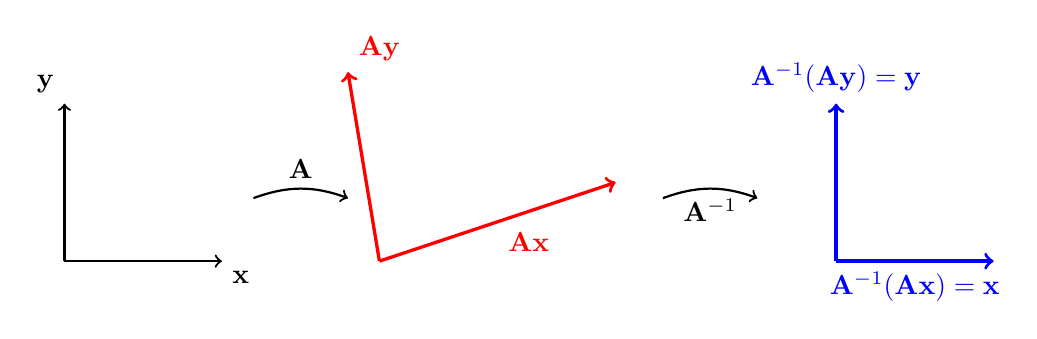
\begin{tikzpicture}[x=2cm,y=2cm]
 			
 			\begin{scope}
 				\draw[->, thick] (0,0) -- (1,0) node[below right] {${\bf x}$};
 				\draw[->, thick] (0,0) -- (0,1) node[above left] {${\bf y}$};
 			\end{scope}
 			
 			\begin{scope}[shift={(2.0,0)}]
 				\coordinate (A) at (1.5,0.5);
 				\coordinate (B) at (-0.2,1.2);
				\draw[->, very thick, red] (0,0) -- (A) node[pos=0.5, below right] {${\bf A} {\bf x}$};
 				\draw[->, very thick, red] (0,0) -- (B) node[above right] {${\bf A} {\bf y}$};
 			\end{scope}
 			
 			\begin{scope}[shift={(4.9,0)}]
 				\draw[->, very thick, blue] (0,0) -- (1,0) node[pos=0.5, below] {${\bf A}^{-1} ({\bf A} {\bf x}) = {\bf x}$};
 				\draw[->, very thick, blue] (0,0) -- (0,1) node[above] {${\bf A}^{-1} ({\bf A} {\bf y}) = {\bf y}$};
 			\end{scope}
 			
 			\draw[->, thick, bend left=20] (1.2,0.4) to node[above] {${\bf A}$} (1.8,0.4);
 			\draw[->, thick, bend left=20] (3.8,0.4) to node[below] {${\bf A}^{-1}$} (4.4,0.4);
 		\end{tikzpicture}
 		\caption{A matrix $\mathbf{A}$ represents a linear transformation of $\mathbb{R}^{2}$. The inverse matrix $\mathbf{A}^{-1}$ 
 			represents the inverse transformation. \label{fig_matrix_inverse_dict}} 
 		\end{figure}
		See also: matrix, determinant, linear regression, pseudoinverse.},
	first={inverse matrix},
	text={inverse matrix}
}

\newglossaryentry{matrix}
{name={matrix},
	description={A matrix of size $m \times d$ is a 2-D array of numbers, 
 		which is denoted  
		$$
  		{\bf A} = \begin{bmatrix}
   		A_{1,1} & A_{1,2} & \dots  & A_{1,d} \\
		A_{2,1} & A_{2,2} & \dots  & A_{2,d} \\
		\vdots  & \vdots  & \ddots & \vdots \\
		A_{m,1} & A_{m,2} & \dots  & A_{m,d}
		\end{bmatrix} \in \mathbb{R}^{m \times d}.
		$$
		Here, $A_{r,j}$ denotes the matrix entry in the $r$th row and the 
		$j$th column. Matrices are useful representations of various mathematical objects \cite{StrangLinAlg2016},
		including the following:
		\begin{itemize}
			\item Systems of linear equations: We can use a matrix to represent a system of linear equations 
			$$ \begin{pmatrix}
			A_{1,1} & A_{1,2} \\
			A_{2,1} & A_{2,2}
			\end{pmatrix}
			\begin{pmatrix}
				w_1 \\
				w_2
			\end{pmatrix}
			=\begin{pmatrix}
				y_1 \\
				y_2
			\end{pmatrix}
			\quad \text{ compactly as } \quad {\bf A} {\bf w} = {\bf y}.
			$$
    			One important example of systems of linear equations are the optimality condition for the 
    			model parameters within linear regression. 
			\item Linear maps:
			Consider a $d$-dimensional vector space $\mathcal{U}$ and a $m$-dimensional vector space $\mathcal{V}$. 
			If we fix a basis $\mathbf{u}^{(1)},\,\ldots,\,\mathbf{u}^{(d)}$ for $\mathcal{U}$ and a basis $\mathbf{v}^{(1)},\,\ldots,\,\mathbf{v}^{(m)}$ 
			for $\mathcal{V}$, each matrix ${\bf A} \in \mathbb{R}^{m \times d}$ naturally defines a 
			linear map $\alpha: \mathcal{U} \rightarrow \mathcal{V}$ (see Fig. \ref{fig_matrix_dict}) such that
   			$${\bf u}^{(j)} \mapsto \sum_{r=1}^{m} A_{r,j} {\bf v}^{(r)}.$$
			\item Datasets: We can use a matrix to represent a dataset. Each row 
			corresponds to a single data point, and each column corresponds to a specific 
			feature or label of a data point. 
		\end{itemize}
		\begin{figure}[H]
		\begin{center}
		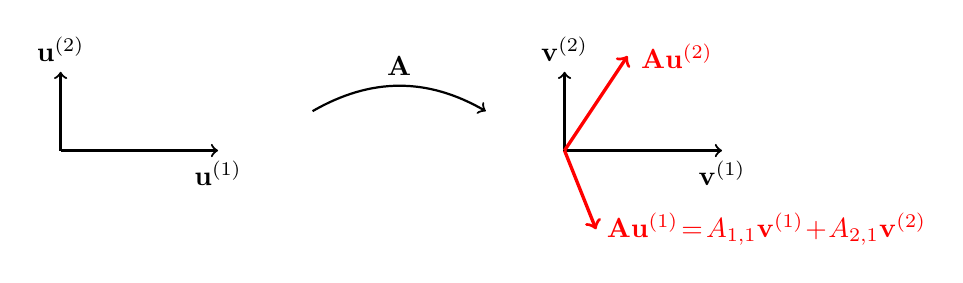
\begin{tikzpicture}[x=2cm]
			
			\begin{scope}
				\draw[->, thick] (0,0) -- (1,0) node[below] {${\bf u}^{(1)}$};
				\draw[->, thick] (0,0) -- (0,1) node[above] {${\bf u}^{(2)}$};
				
				
				
			\end{scope}
			
			\begin{scope}[shift={(3.2,0)}]
				\draw[->, thick] (0,0) -- (1,0) node[below] {${\bf v}^{(1)}$};
				\draw[->, thick] (0,0) -- (0,1) node[above] {${\bf v}^{(2)}$};
				\coordinate (A) at (0.2,-1.0);
				\coordinate (B) at (0.4,1.2);
				\draw[->, very thick, red] (0,0) -- (A) node[below,right] {${\bf A} {\bf u}^{(1)}\!=\!A_{1,1}{\bf v}^{(1)}\!+\!A_{2,1}{\bf v}^{(2)}$};
				\draw[->, very thick, red] (0,0) -- (B) node[right,xshift=1pt] {${\bf A} {\bf u}^{(2)}$};
				
				
			\end{scope}
			
			\draw[->, thick] (1.6,0.5) to[bend left] node[midway, above] {${\bf A}$} (2.7,0.5);
		
		\end{tikzpicture}
		\end{center}
		\caption{A matrix ${\bf A}$ defines a linear map between two vector spaces. \label{fig_matrix_dict}} 
		\end{figure}
		See also: linear map, dataset, linear model. },
	first={matrix},
	firstplural={matrices},
	type=math,
	plural={matrices},
	text={matrix}
}

\newglossaryentry{det}
{name={determinant},
	description={The determinant $\det\,({\bf A})$ of a square matrix 
		${\bf A} = \big( {\bf a}^{(1)},\,\ldots,\,{\bf a}^{(d)} \big) \in \mathbb{R}^{d \times d}$ is a 
		function of its columns ${\bf a}^{(1)},\,\ldots,\,{\bf a}^{(d)} \in \mathbb{R}^{d}$, i.e., it satisfies 
		the following properties \cite{DirschmidHansJorg1996TuF}:
		\begin{itemize}
			\item Normalized: $$\det (\mathbf{I}) = 1$$ 
			\item Multilinear: \begin{align} \nonumber \det \big({\bf a}^{(1)},\,\ldots,\,\alpha{\bf u}+ \beta {\bf v},\,\ldots,\,{\bf a}^{(d)} \big) & = \alpha\det \big({\bf a}^{(1)},\,\ldots,\,{\bf u},\,\ldots,\,{\bf a}^{(d)} \big) \\ 
			& +\beta\det \big({\bf a}^{(1)},\,\ldots,\,{\bf v},\,\ldots,\,{\bf a}^{(d)} \big) \nonumber
			\end{align}
			\item Antisymmetric: $$\det \big(\ldots,\,{\bf a}^{(j)}, \,\ldots, \,{\bf a}^{(j')},\,\ldots \big) = - \det \big(\ldots,\,{\bf a}^{(j')}, \,\ldots, \,{\bf a}^{(j)},\,\ldots \big).$$ 
		\end{itemize} 
		We can interpret a matrix ${\bf A}$ as a linear transformation on $\mathbb{R}^{d}$.
		The determinant $\det\,({\bf A})$ characterizes how (the orientation of) 
 		volumes in $\mathbb{R}^d$ are altered by this transformation (see Fig. \ref{fig_det_dict}) \cite{GolubVanLoanBook}, \cite{Strang2007}. 
 		In particular, $\det\,({\bf A}) > 0$ preserves orientation, $\det\,({\bf A}) < 0$ reverses orientation, 
 		and $\det\,({\bf A}) = 0$ collapses volume entirely, indicating that ${\bf A}$ is non-invertible. 
 		The determinant also satisfies $\det\,({\bf A} {\bf B}) = \det\,({\bf A}) \cdot \det\,({\bf B})$, and if ${\bf A}$ is 
 		diagonalizable with eigenvalues $\lambda_{1}, \,\ldots, \,\lambda_{d}$, then 
		$\det({\bf A}) = \prod_{j=1}^{d} \lambda_{j}$ \cite{HornMatAnalysis}.
    		For the special cases $d=2$ (i.e., two-dimensional or 2-D) and $d=3$ (i.e., three-dimensional or 3-D), 
		the determinant can be interpreted as an oriented area or volume spanned by the column vectors of ${\bf A}$.
    		\begin{figure}[H]
    			\begin{center}
    			\begin{tikzpicture}[x=2cm]
			
			\begin{scope}
			\draw[->, thick] (0,0) -- (1,0) node[below right] {${\bf x}$};
			\draw[->, thick] (0,0) -- (0,1) node[above left] {${\bf y}$};
			
			
			
			\end{scope}
			
			\begin{scope}[shift={(2.8,0)}]
			\coordinate (A) at (1.5,0.5);
			\coordinate (B) at (-0.2,1.2);
			\draw[->, very thick, red] (0,0) -- (A) node[below right] {${\bf A} {\bf x}$};
			\draw[->, very thick, red] (0,0) -- (B) node[above left] {${\bf A} {\bf y}$};
			\draw[fill=red!20, opacity=0.6] (0,0) -- (A) -- ($(A)+(B)$) -- (B) -- cycle;
			\draw[dashed] (A) -- ($(A)+(B)$);
			\draw[dashed] (B) -- ($(A)+(B)$);
			\node at (0.8,0.6) {\small $\det\,({\bf A})$};
			
			\draw[->, thick, blue] (0.4,0.0) arc[start angle=0, end angle=35, radius=0.6];
			
			
			\end{scope}
			
			\draw[->, thick] (1.3,0.5) -- (2.4,0.5) node[midway, above] {${\bf A}$};
			\end{tikzpicture}
			\end{center}
			\caption{We can interpret a square matrix ${\bf A}$ as a linear transformation of $\mathbb{R}^{d}$ 
				into itself. The determinant $\det\,({\bf A})$ characterizes how this transformation alters an oriented volume.
				\label{fig_det_dict}}
		\end{figure}
		See also: eigenvalue, inverse matrix.},
	first={determinant},
	type=math,
	text={determinant}
}

\newglossaryentry{linearmap}
{name={linear map}, plural={linear maps}, 
	description={A linear map $f: \mathbb{R}^n \rightarrow \mathbb{R}^m$ is a function that satisfies additivity, i.e.,
		$f({\bf x} + {\bf y}) = f({\bf x}) + f({\bf y})$, and homogeneity, i.e.,
		$f(c{\bf x}) = c f({\bf x})$, for all vectors ${\bf x}, {\bf y} \in \mathbb{R}^n$ and scalars $c \in \mathbb{R}$. 
		In particular, $f(\mathbf{0}) = \mathbf{0}$. Any linear map can be represented as a matrix 
		multiplication $f({\bf x}) = {\bf A} {\bf x}$ for some matrix ${\bf A} \in \mathbb{R}^{m \times n}$. 
		The collection of real-valued linear maps for a given dimension $n$ constitute a linear model, 
		which is used in many ML methods.
		\\
		See also: map, function, vector, matrix, linear model, ML.},
	first={linear map},
	text={linear map}
}

\newglossaryentry{vector}
{name={vector},
	description={A vector is an element of a vector space. 
		In the context of ML, a particularly important example of a vector space 
		is the Euclidean space $\mathbb{R}^{d}$, where $d \in \mathbb{N}$ 
		is the (finite) dimension of the space. A vector ${\bf x} \in \mathbb{R}^{d}$ 
		can be represented as a list or one-dimensional (1-D) array of real numbers, i.e., 
		$x_1, \,\ldots, \,x_{d}$ with $x_j \in \mathbb{R}$ for 
		$j = 1, \,\ldots, \,d$. The value $x_j$ is the $j$th 
		entry of the vector ${\bf x}$. It can also be useful to view a vector ${\bf x} \in \mathbb{R}^{d}$ 
		as a function that maps each index $j \in \{1, \,\ldots, \,d\}$ 
		to a value $x_j \in \mathbb{R}$, i.e., ${\bf x}: j \mapsto x_j$. 
		This perspective is particularly useful for the study of kernel methods.
		\begin{figure}[H]
			
			\begin{minipage}[c]{0.48\textwidth}
				\centering 
				2, --1, 3, 0, --2, 1
				\begin{minipage}{\textwidth}
				\vspace{5ex}
				\centering
				{\selectfont (a)}
				\end{minipage}
			\end{minipage}
			\hfill
			
			\begin{minipage}{0.48\textwidth}
			\centering
			\begin{tikzpicture}
			\begin{axis}[
    				width=6.5cm,
    				height=5cm,
    				title={},
    				xlabel={index $j$},
    				ylabel={$x_j$},
   		 		ymin=-3.5, ymax=3.5,
    				xmin=0.5, xmax=6.5,
   	 			xtick={1,2,3,4,5,6},
    				ytick={-3,-2,-1,0,1,2,3},
    				axis x line=bottom,        
    				axis y line=left,          
    				grid=both,
    				major grid style={dotted, gray!60},
    				enlargelimits=0.1
			]
			\addplot+[ycomb, thick, mark=*]
    			coordinates {
        				(1,2)
        				(2,-1)
       	 			(3,3)
        				(4,0)
        				(5,-2)
        				(6,1)
    			};
			\end{axis}
			\node at (2,-2.5) {(b)};
			\end{tikzpicture}
			\end{minipage}
			\caption{Two equivalent views of a vector ${\bf x}= \big( 2, -1, 3, 0, -2, 1 \big)^{T} \in \mathbb{R}^{6}$.
			(a) As a numeric array. (b) As a map $j \mapsto x_j$.}
			\label{fig:vector-function-dual_dict}
		\end{figure}
		See also: vector space, Euclidean space, linear map.},
	first={vector},
	firstplural={vectors},
	type=math,
	plural={vectors},
	text={vector}
}


\newglossaryentry{vectorspace}
{name={vector space},
	description={A vector space $\mathcal{V}$ (also called linear space) 
	is a collection of elements, called vectors, along with the following two operations: 
    	1) addition (denoted ${\bf v}+{\bf w}$) of two vectors ${\bf v},{\bf w}$; and 2) multiplication 
	(denoted $c \,\cdot \,{\bf v}$) of a vector ${\bf v}$ with a scalar $c$ that belongs to some 
	number field (with a typical choice for this field being $\mathbb{R}$). The defining 
	property of a vector space is that it is closed under these operations:
		\begin{itemize}
			\item If ${\bf v}, {\bf w} \in \mathcal{V}$, then ${\bf v} + {\bf w} \in \mathcal{V}$.
			\item If ${\bf v} \in \mathcal{V}$ and $c \in \mathbb{R}$, then $c {\bf v} \in \mathcal{V}$.
			\item In particular, $\mathbf{0} \in \mathcal{V}$.
		\end{itemize}
		\begin{figure}[H]
		\centering
			\begin{tikzpicture}[>=Stealth, scale=1.2]
				  
  			\coordinate (O) at (0,0);            
  			\coordinate (V) at (2,1.5);          
  			\coordinate (W) at (1,3);            
  			\coordinate (VplusW) at (3,4.5);     
  			\coordinate (HalfV) at (1,0.75);     
  			\draw[->, thick, blue] (O) -- (V) node[pos=1, right] {${\bf v}$};
  			\draw[->, thick, red] (O) -- (W) node[pos=1, left] {${\bf w}$};
  			\draw[->, thick, purple] (O) -- (VplusW) node[pos=0.99, above right] {${\bf v}+{\bf w}$};
  			\draw[dashed, red] (V) -- (VplusW);
  			\draw[dashed, blue] (W) -- (VplusW);
  			\draw[->, thick, orange] (O) -- (HalfV) node[midway, right] {$ \alpha {\bf v}$};
			
  			\filldraw[black] (O) circle (2pt) node[below left] {$\mathbf{0}$};  
  			\filldraw[blue] (V) circle (2pt);         
  			\filldraw[red] (W) circle (2pt);          
  			\filldraw[purple] (VplusW) circle (2pt);  
  			\filldraw[orange] (HalfV) circle (2pt);   
			\end{tikzpicture}
			\caption{A vector space $\mathcal{V}$ is a collection of vectors such that 
			scaling and adding them always yields another vector in $\mathcal{V}$.}
			
			
			\label{fig:vector-ops_dict}
		\end{figure}
		A common example of a vector space is the Euclidean space $\mathbb{R}^n$, which is 
		widely used in ML to represent datasets. We can also use $\mathbb{R}^n$ 
		to represent, either exactly or approximately, the hypothesis space used by an ML method.  
		Another example of a vector space, which is naturally associated with every probability space 
		$\mathcal{P}=\big(\Omega,\mathcal{R},\mathbb{P}({\cdot}) \big)$, is the collection of all 
		real-valued RVs $x: \Omega \rightarrow \mathbb{R}$ \cite{RudinBook}, \cite{folland1999real}.  
		\\
		See also: vector, Euclidean space, linear model, linear map.},
	first={vector space},
	type=math,
	text={vector space}
}


\newglossaryentry{stochastic}
{name={stochastic},
	description={We refer to a  method as stochastic if it involves a 
		random component or is governed by probabilistic laws. ML methods use randomness 
		to reduce computational complexity (e.g., see SGD) or 
		to capture uncertainty in probabilistic models.
		\\
		See also: SGD, uncertainty, probabilistic model.},
	first={stochastic},
	text={stochastic}
}

\newglossaryentry{stochproc}
{name={stochastic process},
	description={A stochastic process is a collection of 
		RVs defined on a common probability space and indexed by some set 
		$\mathcal{I}$ \cite{GrayProbBook}, \cite{papoulis}, \cite{Brockwell91}. The index set 
		$\mathcal{I}$ typically represents time or space, allowing us to represent 
		random phenomena that evolve across time or spatial dimensions—for example, 
		sensor noise or financial time series. Stochastic processes are not limited 
		to temporal or spatial settings. For instance, random graphs such as 
		the ER graph or the SBM can also be viewed as stochastic processes. 
		Here, the index set $\mathcal{I}$ consists of node pairs that index RVs whose values 
		encode the presence or weight of an edge between two nodes. Moreover, stochastic 
		processes naturally arise in the analysis of stochastic algorithms, 
		such as SGD, which construct a sequence of RVs. 
		\\
		See also:  RV, SBM, SGD, uncertainty, probabilistic model.},
	first={stochastic process},
	firstplural={stochastic processes},
	type=math, 
	plural={stochastic processes},
	text={stochastic process}
}

\newglossaryentry{characteristicfunc}
{name={characteristic function},
	description={The characteristic function 
		of a real-valued RV $x$ is the function \cite[Sec. 26]{BillingsleyProbMeasure}
		$$ \phi_{x}(t) := \mathbb{E}  { \exp\,(j t x) } \mbox{ with } j = \sqrt{-1}.$$
	 	The characteristic function uniquely determines the probability distribution of $x$. 
		\\
		See also: RV, probability distribution.},
	first={characteristic function},
	firstplural={characteristic functions}, 
	type=math, 
	plural={characteristic functions},
	text={characteristic function}
}

\newglossaryentry{entropy}
{name={entropy},
	description={Entropy quantifies the uncertainty or unpredictability associated with an RV \cite{coverthomas}. 
		For a discrete RV $x$ taking on values in a finite set $\mathcal{S} = \{x_1, \,\ldots, \,x_n\}$ with 
		a probability mass function $p_i := \mathbb{P}({x = x_i})$, the entropy is defined as
		\[
		H(x) := -\sum_{i=1}^n p_i \log p_i.
		\]
		Entropy is maximized when all outcomes are equally likely, and minimized (i.e., zero) 
		when the outcome is deterministic. A generalization of the concept of entropy for continuous 
		RVs is differential entropy. 
		\\
		See also: uncertainty, probabilistic model.},
	first={entropy},
	text={entropy}
}

\newglossaryentry{diffentropy}
{name={differential entropy},
	description={For a real-valued RV ${\bf x} \in \mathbb{R}^{d}$ 
		with a pdf $p(x)$, the differential entropy is defined as \cite{coverthomas}
		\[
		h({\bf x}) := - \int p({\bf x}) \log p({\bf x}) \, d{\bf x}.
		\]
		Differential entropy can be negative and lacks some properties of entropy for 
		discrete-valued RVs, such as invariance under a change of variables \cite{coverthomas}. 
		Among all RVs with a given mean ${\bm \mu}$ and covariance matrix ${\bf \Sigma}$, 
		$h({\bf x})$ is maximized by ${\bf x} \sim \mathcal{N}\left({\bm \mu},{\bf \Sigma}\right)$. 
		\\
		See also: uncertainty, probabilistic model.},
	first={differential entropy},
	text={differential entropy}
}

\newglossaryentry{minimum}
{name={minimum},
	description={Given a set of real numbers, the minimum is the smallest of those numbers.
		Note that for some sets, such as the set of negative real numbers, the minimum does not exist.},
	firstplural={minima}, 
 	plural={minima},
	first={minimum},
	text={minimum}
}

\newglossaryentry{function}
{name={function}, 
	description={A function between two sets $\mathcal{U}$ and $\mathcal{V}$ assigns  
		each element $u \in \mathcal{U}$ exactly one element $f(u) \in \mathcal{V}$ \cite{RudinBookPrinciplesMatheAnalysis}.
		We write this as $$f: \mathcal{U} \rightarrow \mathcal{V}: u \mapsto f(u)$$ 
		where $\mathcal{U}$ is the domain and $\mathcal{V}$ the co-domain of $f$. 
		That is, a function $f$ defines a unique output $f(u) \in \mathcal{V}$ for every 
		input $u \in \mathcal{U}$ (see Fig. \ref{fig_function_dict}).
		\begin{figure}[H]
			\centering
			\begin{tikzpicture}[>=stealth, node distance=1.2cm and 2.5cm]
				\tikzset{dot/.style={circle, fill=black, inner sep=1.2pt}}
				\node (A) [dot, label=left:$a$] {};
				\node (B) [dot, below=of A, label=left:$b$] {};
				\node (C) [dot, below=of B, label=left:$c$] {};
				\node (1) [dot, right=4cm of A, label=right:$1$] {};
				\node (2) [dot, below=of 1, label=right:$2$] {};
				\node (3) [dot, below=of 2, label=right:$3$] {};
				\node[draw=blue!70, thick, ellipse, inner sep=0.5cm, fit=(A)(B)(C), label=above:$\mathcal{U}$] {};
				\node[draw=green!70!black, thick, ellipse, inner sep=0.5cm, fit=(1)(2)(3), label=above:$\mathcal{V}$] {};
				\draw[->] (A) -- (2);
				\draw[->] (B) -- (1);
				\draw[->] (C) -- (2);
			\end{tikzpicture}
			\caption{A function \( f \colon \{a,b,c\} \to \{1,2,3\} \) mapping each element of the domain to exactly one element of 
				the co-domain. \label{fig_function_dict}}
		\end{figure} },
	first={function},
	firstplural={functions}, 
	type=math, 
	plural={functions},
	text={function}
}


\newglossaryentry{map}
{name={map}, 
	description={We use the term map as a synonym for function.
		\\
		See also: function.},
	first={map},
	firstplural={maps},	
	type=math, 
	plural={maps},
	text={map}
}


\newglossaryentry{attention}
{name={attention}, 
	description={Some ML applications involve data points composed of smaller units, known 
		as tokens. For example, a sentence consists of words, an image of pixel patches, and a network of 
		nodes. In practice, the tokens within a single data point are typically not independent of one 
		another, but rather, each token pays attention to specific other tokens. Probabilistic models provide a 
		principled framework for representing and analyzing such dependencies \cite{Blei2003}. Attention 
		mechanisms use a more direct approach without explicit reference to a probabilistic model. The idea is to 
		represent the relationship between two tokens $i$ and $i'$ using a parameterized function $f^{({\bf w})}(i,i')$, 
		where the parameters ${\bf w}$ are learned via a variant of ERM. 
		Practical attention mechanisms differ in their precise choice of attention model $f^{({\bf w})}(i,i')$ 
		as well as in the precise ERM variant used to learn the parameters ${\bf w}$. One widely-used family of attention mechanisms 
		defines the parameters ${\bf w}$ in terms of two vectors associated with each token $i$, i.e.,
		a query vector ${\bf q}^{(i)}$ and a key vector ${\bf k}^{(i')}$. For a given token $i$ 
		with query ${\bf q}^{(i)}$, and another token $i'$ with key ${\bf k}^{(i')}$, the quantity 
		$\big( {\bf q}^{(i)} \big)^{\top} {\bf k}^{(i')}$ quantifies the extent to which token $i$ attends 
		to (or depends on) token $i'$.
		\begin{figure}[H]
			\centering
			\begin{tikzpicture}[>=stealth, node distance=0.2cm and 0.2cm,
			every node/.style={inner sep=2pt, font=\large}, baseline]
			
			\node (w1) [draw, fill=gray!10, rounded corners] {All};
			\node (w2) [draw, fill=gray!10, right=of w1, rounded corners] {human};
			\node (w3) [draw, fill=gray!10, right=of w2, rounded corners] {beings};
			\node (w4) [draw, fill=gray!10, right=of w3, rounded corners] {are};
			\node (w5) [draw, fill=gray!10, right=of w4, rounded corners] {born};
			\node (w6) [draw, fill=gray!10, right=of w5, rounded corners] {free};
			\node (w7) [draw, fill=gray!10, right=of w6, rounded corners] {and};
			\node (w8) [draw, fill=blue!20, right=of w7, rounded corners] {equal};
			
   	   		\node[font=\footnotesize, below=0.15cm of w8, align=center] (labeli) {$i$ \\ ${\bf q}^{(i)},\ {\bf k}^{(i)}$};
			\node[font=\footnotesize, below=0.15cm of w1, align=center] (labelii) {$i'$ \\ ${\bf q}^{(i')},\ {\bf k}^{(i')}$};
			
	  		\node (eqTop) [above=1.8cm of w8] {};
	 		
	 		\draw[->, thick, opacity=0.3] (w8.north) .. controls +(up:1.0cm) and +(up:1.0cm) .. (w6.north); 
	 		\draw[->, thick, opacity=0.3] (w8.north) .. controls +(up:1.2cm) and +(up:1.0cm) .. (w5.north); 
			\draw[->, thick, opacity=1]  (w8.north)  .. controls +(up:1.8cm) and +(up:1.0cm) ..  node[midway, text=black, above] {$f^{({\bf w})}(i,i')$}  (w1.north); 
			\end{tikzpicture}
			\caption{Attention mechanisms learn a parameterized function $f^{({\bf w})}(i,i')$ to measure 
			how much token $i$ attends to token $i'$. One widely-used construction of $f^{({\bf w})}(i,i')$ 
			uses query and key vectors, denoted ${\bf q}^{(i)}$ and ${\bf k}^{(i)}$, assigned to each token $i$ \cite{vaswani2017attention}.}
		\end{figure}
		See also: function.},
	first={attention},
	text={attention}
}


\newglossaryentry{optproblem}
{name={optimization problem}, 
	description={An optimization problem is a mathematical 
		   structure consisting of an objective function $f: \mathcal{U} \rightarrow \mathcal{V}$ 
		   defined over an optimization variable ${\bf w} \in \mathcal{U}$, together with a 
		   feasible set $\mathcal{W} \subseteq \mathcal{U}$. The co-domain $\mathcal{V}$ is 
		   assumed to be ordered, meaning that for any two elements $\mathbf{a}, \mathbf{b} \in \mathcal{V}$, 
		   we can determine whether $\mathbf{a} < \mathbf{b}$, $\mathbf{a} = \mathbf{b}$, 
		   or $\mathbf{a} > \mathbf{b}$. The goal of optimization is to find those values ${\bf w} \in \mathcal{W}$ 
		   for which the objective $f({\bf w})$ is extremal—i.e., minimal or maximal \cite{BoydConvexBook}, \cite{BertsekasNonLinProgr}, \cite{nesterov04}.
		   \\
		   See also: objective function.},
	first={optimization problem},
	firstplural={optimization problems}, 
	type=math,
	plural={optimization problems}, 
	text={optimization problem}
}

\newglossaryentry{optmethod}
{name={optimization method},
	description={An optimization method is an algorithm that 
		reads in a representation of an optimization problem and delivers an (approximate) solution 
		as its output \cite{BoydConvexBook}, \cite{BertsekasNonLinProgr}, \cite{nesterov04}.
		 \\
		 See also: algorithm, optimization problem.},
	first={optimization method},
	firstplural={optimization methods}, 
	plural={optimization methods}, 
	text={optimization method}
}

\newglossaryentry{fixedpointiter}
{name={fixed-point iteration},
	description={A fixed-point iteration is an iterative method for solving 
		a given optimization problem. It constructs a sequence ${\bf w}^{(0)}, \,{\bf w}^{(1)}, \,\ldots$ by 
		 repeatedly applying an operator $\mathcal{F}$, i.e., 
		 \begin{equation} 
		 	\label{equ_def_fixed_point_dict} 
		 	{\bf w}^{(k+1)} = \mathcal{F} {\bf w}^{(k)} \mbox{, for } k=0, \,1, \,\ldots.
		 \end{equation} 
		 The operator $\mathcal{F}$ is chosen such that any of its fixed points is a solution 
		 $\widehat{{\bf w}}$ to the given optimization problem. For example, given a differentiable and 
		 convex function $f({\bf w})$, the fixed points of the operator $\mathcal{F}: {\bf w} \mapsto {\bf w} - \nabla f({\bf w})$ 
		 coincide with the minimizers of $f({\bf w})$. In general, for a given optimization problem with solution $\widehat{{\bf w}}$, 
		 there are many different operators $\mathcal{F}$ whose fixed points are $\widehat{{\bf w}}$. 
		 Clearly, we should use an operator $\mathcal{F}$ in \eqref{equ_def_fixed_point_dict} that reduces the distance to a solution such that
		 \begin{equation} 
			\nonumber
			\underbrace{\left\Vert  { {\bf w}^{(k+1)} - \widehat{\mathbf{w}}} \right\Vert_{2}}_{\stackrel{\eqref{equ_def_fixed_point_dict}}{=} \left\Vert  { \mathcal{F} {\bf w}^{(k)} - \mathcal{F}\widehat{{\bf w}}} \right\Vert_{2}}  \leq 	\left\Vert  { {\bf w}^{(k)} - \widehat{{\bf w}}} \right\Vert_{2}. 
		\end{equation}
		Thus, we require $\mathcal{F}$ to be at least non-expansive, i.e., the iteration \eqref{equ_def_fixed_point_dict} 
		should not result in worse model parameters that have a larger distance to a solution $\widehat{{\bf w}}$. 
		Furthermore, each iteration \eqref{equ_def_fixed_point_dict} should also make some progress, i.e., 
		reduce the distance to a solution $\widehat{{\bf w}}$. This requirement can be made precise using 
		the notion of a contraction operator \cite{Bauschke:2017}, \cite{fixedpoinIsta}. 
		The operator $\mathcal{F}$ is a contraction operator if, for some $\kappa \in [0,1)$,
		\begin{equation} 
			\nonumber
			\left\Vert  { \mathcal{F} {\bf w}\!-\!\mathcal{F} {\bf w}'} \right\Vert_{2}  \leq  \kappa	\left\Vert  {{\bf w}\!-\!{\bf w}'} \right\Vert_{2} \mbox{ holds for any } {\bf w},{\bf w}'.
		\end{equation}
		For a contraction operator $\mathcal{F}$, the fixed-point iteration \eqref{equ_def_fixed_point_dict} generates 
		a sequence ${\bf w}^{(k)}$ that converges quite rapidly. In particular \cite[Th. 9.23]{RudinBookPrinciplesMatheAnalysis}, 
		\begin{equation} 
			\nonumber
			\left\Vert  { {\bf w}^{(k)} - \widehat{{\bf w}}} \right\Vert_{2} \leq \kappa^{k} 	\left\Vert  { {\bf w}^{(0)} - \widehat{{\bf w}}} \right\Vert_{2}. 
		\end{equation} 
		Here, $\left\Vert  { {\bf w}^{(0)} - \widehat{{\bf w}}} \right\Vert_{2}$ is the distance between 
		the initialization ${\bf w}^{(0)}$ and the solution $\widehat{{\bf w}}$. 
		It turns out that a fixed-point iteration \eqref{equ_def_fixed_point_dict} with a firmly non-expansive 
		operator $\mathcal{F}$ is guaranteed to converge to a fixed-point of $\mathcal{F}$ \cite[Cor. 5.16]{Bauschke:2017}. 
		Fig. \ref{fig_examples_nonexp_dict} depicts examples of a firmly non-expansive operator, a non-expansive operator, 
		and a contraction operator. All of these operators are defined on the 1-D space $\mathbb{R}$. 
		Another example of a firmly non-expansive operator is the proximal operator of a convex function \cite{Bauschke:2017}, \cite{ProximalMethods}. 
		\definecolor{darkgreen}{rgb}{0.0, 0.5, 0.0}
		\begin{figure}[H]
			\begin{center} 
				\begin{tikzpicture}[scale=1.5]
					
					\draw[line width=1pt, ->] (-2,0) -- (2,0) node[right] {$w^{(k)}$};
					\draw[line width=1pt, ->] (0,-2) -- (0,2) node[above] {$w^{(k+1)}$};
					
					\node at (2.1,2.2) {$\mathcal{F}^{(3)}$};
					\node at (1.9,-1.5) {$\mathcal{F}^{(1)}$};
					\node at (1.5,1.2) {$\mathcal{F}^{(2)}$};
					
					\draw[dashed] (1,-2) -- (1,2); 
					\draw[dashed] (-2,1) -- (2,1); 
					\draw[dashed] (-2,-1) -- (2,-1); 
					\draw[dashed] (-1,-2) -- (-1,2); 
					\node[above,xshift=4pt,yshift=-1pt] at (1,0) {$1$};
					\node[above,xshift=8pt,yshift=-1pt] at (0,-1) {$-1$};
					
					\draw[line width=2,domain=-2:2,smooth,blue] plot(\x,{0.5*\x + 1});
					
					\draw[line width=2,domain=-2:2,smooth,red] plot(\x,{-\x});
					
					\draw[line width=2, domain=-2:-1,smooth,darkgreen] plot(\x,{-1});
					\draw[line width=2,domain=-1:1,smooth,darkgreen] plot(\x,{\x});
					\draw[line width=2,domain=1:2,smooth,darkgreen] plot(\x,{1});
				\end{tikzpicture}
			\end{center} 
			\caption{Example of a non-expansive operator $\mathcal{F}^{(1)}$, a firmly non-expansive operator $\mathcal{F}^{(2)}$, and 
				a contraction operator $\mathcal{F}^{(3)}$. \label{fig_examples_nonexp_dict}}
		\end{figure} 
		See also: optimization problem, differentiable, convex function, model parameters, contraction operator, proximal operator.},
	first={fixed-point iteration},
	text={fixed-point iteration},
	firstplural={fixed-point iterations}, 
	plural={fixed-point iterations}
}


\newglossaryentry{ergraph}
{name={Erd\H{o}s–R\'enyi graph (ER graph)},
	description={An ER graph\index{Erd\H{o}s–R\'enyi graph (ER graph)} is a probabilistic model for graphs defined over 
		a given node set $i=1, \,\ldots, \,n$. One way to define the ER graph is 
		via the collection of iid binary RVs $b^{(\{i,i'\})} \in \{0,1\}$, 
		for each pair of different nodes $i, i'$. A specific realization  
		of an ER graph contains an edge $\{i,i'\}$ if and only if 
		$b^{(\{i,i'\})}=1$. The ER graph is parameterized by the 
		number $n$ of nodes and the probability $\mathbb{P}({b^{(\{i,i'\})}=1})$. 
		\\
		See also: graph, probabilistic model, iid, RV, realization, probability.},
	first={Erd\H{o}s–R\'enyi (ER) graph},
	text={ER graph}
}

\newglossaryentry{attack}
{name={attack},  
	description={An attack on an ML system refers to an intentional action—either 
		active or passive—that compromises the system's integrity, availability, or confidentiality. 
		Active attacks involve perturbing components such as datasets (via data poisoning) 
		or communication links between devices within an ML application. Passive attacks, 
		such as privacy attacks, aim to infer sensitive attributes without modifying the system. 
		Depending on their goal, we distinguish between denial-of-service attacks, backdoor attacks, and privacy attacks.
		\\
		See also: data poisoning, privacy attack, sensitive attribute, denial-of-service attack, backdoor.},
	plural={attacks}, 
	first={attack},
	firstplural={attacks},
	text={attack}
}

\newglossaryentry{privattack}
{name={privacy attack},
	description={A privacy attack on an ML system aims to infer 
		sensitive attributes of individuals by exploiting partial access to a trained ML model. 
		One form of a privacy attack is model inversion.\\
		See also: attack, sensitive attribute, model inversion, trustworthy AI, GDPR.},
	plural={privacy attacks}, 
	first={privacy attack},
	firstplural={privacy attacks}, 
	text={privacy attack}
}

\newglossaryentry{epigraph}
{name={epigraph},
  description={The epigraph of a real-valued function $f : \mathbb{R}^n \to \mathbb{R} \cup \{+\infty\}$ 
  	is the set of points lying on or above its graph (see Fig. \ref{fig_epigraph_dict}), i.e., 
		\[
		\operatorname{epi}(f) = \left\{ (\mathbf{x}, t) \in \mathbb{R}^n \times \mathbb{R} \,\middle|\, f(\mathbf{x}) \leq t \right\}.
		\]
		A function is convex if and only if its epigraph is a convex set \cite{BoydConvexBook}, \cite{BertCvxAnalOpt}.
		\begin{figure}[H]
			\centering
			\begin{tikzpicture}[scale=1.0]
				\begin{axis}[
					axis lines = middle,
					xlabel = $x$,
					ylabel = {},
					xmin=-2, xmax=2,
					ymin=0, ymax=4.5,
					samples=100,
					domain=-1.5:1.5,
					thick,
					width=8cm,
					height=6cm,
					grid=none,
					axis on top,
					]
					
					\addplot [blue, thick, domain=-1.5:1.5] {x^2} node [pos=0.85, anchor=south west, xshift=5pt] {$f(x)$};
					
					\addplot [
					name path=f,
					draw=none,
					ytick=\empty,
					domain=-1.5:1.5,
					] {x^2};
					\path[name path=top] (axis cs:-1.5,4) -- (axis cs:1.5,4);
					\addplot [
					blue!20,
					opacity=0.6,
					draw=none,
					] fill between [
					of=f and top,
					soft clip={domain=-1.5:1.5},
					];
					    \node[font=\small] at (axis cs:-1.0,2.3) {$\operatorname{epi}(f)$};
				
				\end{axis}
			\end{tikzpicture}
			\caption{Epigraph of the function $f(x) = x^2$ (i.e., the shaded area). \label{fig_epigraph_dict}}
		\end{figure}
		See also: function, convex.},
	first={epigraph},
	text={epigraph},
	plural={epigraphs}
}


\newglossaryentry{nullspace}
{name={nullspace},
	description={The nullspace of a matrix ${\bf A} \in \mathbb{R}^{d' \times d}$, 
		denoted ${\rm null}({\bf A})$, is the set of all vectors $\mathbf{n} \in \mathbb{R}^d$ 
    		such that $${\bf A} \mathbf{n} = \mathbf{0}.$$ 
		Consider a feature learning method that uses the matrix ${\bf A}$ to transform 
		a feature vector $\mathbf{x} \in \mathbb{R}^{d}$ of a data point 
		into a new feature vector ${\bf z} = {\bf A} \mathbf{x} \in \mathbb{R}^{d'}$. 
		The nullspace ${\rm null}({\bf A})$ characterizes all directions in the original 
    		feature space $\mathbb{R}^{d}$ along which the transformation 
		${\bf A} \mathbf{x}$ remains unchanged. In other words, adding any vector from 
		the nullspace to a feature vector ${\bf x}$ does not affect the transformed 
		representation ${\bf z}$. This property can be exploited to enforce invariances in the 
		predictions (computed from ${\bf A} \mathbf{x}$). Fig.\ \ref{fig:nullspace-rotation-dict} 
		illustrates one such invariance. It shows rotated versions of two handwritten digits, 
		which approximately lie along 1-D curves in the original feature space. 
		These curves are aligned with a direction vector $\mathbf{n} \in \mathbb{R}^{d}$. 
    		To ensure that the trained model is invariant to such rotations, we can 
		choose the transformation matrix ${\bf A}$ such that $\mathbf{n} \in {\rm null}({\bf A})$. 
		This ensures that ${\bf A} \mathbf{x}$, and hence the resulting prediction, 
		is approximately insensitive to rotations of the input image.
		\begin{figure}[H]
      			\centering
      			\includegraphics[width=0.6\textwidth]{assets/pythonsnacks/nullspace_0_1.png}
	  		\caption{Rotated images of two handwritten digits. The rotations are approximately 
	  		aligned along linear curves that are parallel to the vector $\mathbf{n}$.\label{fig:nullspace-rotation-dict}}	
	       	\end{figure}
		See also: matrix. \\ 
		Python demo: \href{https://github.com/AaltoDictionaryofML/AaltoDictionaryofML.github.io/blob/main/assets/pythonsnacks/nullspace.py}{click me}},
 	first={nullspace},
 	firstplural={nullspaces},
 	plural={nullspaces},
 	text={nullspace}
}


\newglossaryentry{maximum}
{name={maximum},
	description={The maximum of a set $\mathcal{A} \subseteq \mathbb{R}$ 
     		of real numbers is the greatest element in that set, if such an element exists. A set $\mathcal{A}$ 
     		has a maximum if it is bounded above and attains its supremum \cite[Sec.~1.4]{RudinBookPrinciplesMatheAnalysis}.
				\\ 
		See also: supremum.},
 	first={maximum},
 	firstplural={maxima},
 	plural={maxima},
 	text={maximum}
}

\newglossaryentry{supremum}
{name={supremum (or least upper bound)},
	description={The supremum of a set of real numbers is 
		the smallest number that is greater than or equal to every element in the set. More formally, a 
		real number $a$ is the supremum of a set $\mathcal{A} \subseteq \mathbb{R}$ if: 1) $a$ 
		is an upper bound of $\mathcal{A}$; and 2) no number smaller than $a$ is an upper bound of $\mathcal{A}$. 
		Every non-empty set of real numbers that is bounded above has a supremum, even if it does 
		not contain its supremum as an element \cite[Sec.~1.4]{RudinBookPrinciplesMatheAnalysis}.},
	firstplural={suprema}, 
  	plural={suprema},
	first={supremum (or least upper bound)},
	text={supremum}
}

\newglossaryentry{discrepancy}
{name={discrepancy},
	description={Consider an FL application with networked data 
		represented by an FL network. FL methods use a discrepancy measure 
		to compare hypothesis maps from local models at nodes $i,i'$, 
		connected by an edge in the FL network.
					\\ 
		See also: FL, FL network, local model.},
	first={discrepancy},
	firstplural={discrepancies}, 
  	plural={discrepancies}, 
	text={discrepancy}
}

\newglossaryentry{FedRelax}
{name={federated relaxed (FedRelax)},
	description={An FL distributed algorithm. 
		\\ 
		See also: FL, distributed algorithm.},
	first={FedRelax},
	text={FedRelax}
} 

\newglossaryentry{fedavg}
{name={federated averaging (FedAvg)},
	description={FedAvg refers to a family of iterative FL algorithms. 
		It uses a server-client setting and alternates between clientwise local models 
		retraining, followed by the aggregation of updated model parameters at the server 
		\cite{pmlr-v54-mcmahan17a}. The local update at client $i=1, \,\ldots, \,n$ 
		at time $k$ starts from the current model parameters ${\bf w}^{(k)}$ provided 
		by the server and typically amounts to executing few iterations of SGD. After completing the local updates, they are aggregated 
		by the server (e.g., by averaging them). Fig. \ref{fig_single_iteration_fedavg_dict} illustrates the execution of a single 
		iteration of FedAvg. 
		\begin{figure}[H]
			\begin{center}
			\begin{tikzpicture}[>=Stealth, node distance=1cm and 1.5cm, every node/.style={font=\small}]
			
			\tikzstyle{server} = [circle, fill=black, minimum size=6pt, inner sep=0pt]
			\tikzstyle{client} = [circle, draw=black, minimum size=6pt, inner sep=0pt]
			
			\node (label1) at (0,3.5) {broadcast};
			\node[right=2.5cm of label1] (label2) {local update};
			\node[right=2.5cm of label2] (label3) {aggregate};
			
			\node[server] (s1) at (label1 |- 0,2.5) {};
			\node[client] (c1l) at ($(s1) + (-1cm,-1cm)$) {};
			\node[client] (c1r) at ($(s1) + (1cm,-1cm)$) {};
			\node[] (dots1) at ($(s1) + (0cm,-1cm)$) {\ldots};
			\draw[->] (s1) -- (c1l) node[midway,left] {${\bf w}^{(k)}$};
			\draw[->] (s1) -- (c1r) node[midway,right] {${\bf w}^{(k)}$};
			\draw[->] (s1) -- (dots1);
			
			\node[server] (s2) at (label2 |- 0,2.5) {};
			\node[client] (c2l) at ($(s2) + (-1cm,-1cm)$) {};
			\node[client] (c2r) at ($(s2) + (1cm,-1cm)$) {};
			\node[] (dots2) at ($(s2) + (0cm,-1cm)$) {\ldots};
			\node[below=0.2cm of c2l] {$\mathbf{w}^{(k,1)}$};
			\node[below=0.2cm of c2r] {$\mathbf{w}^{(k,n)}$};
			
			\node[server] (s3) at (label3 |- 0,2.5) {};
			\node[above=0.01cm of s3, yshift=-4pt] {${\bf w}^{(k+1)}$};
			\node[client] (c3l) at ($(s3) + (-1cm,-1cm)$) {};
			\node[client] (c3r) at ($(s3) + (1cm,-1cm)$) {};
			\node[] (dots3) at ($(s3) + (0cm,-1cm)$) {\ldots};
			\draw[->] (c3l) -- (s3) node[midway,left] {$\mathbf{w}^{(k,1)}$};
			\draw[->] (c3r) -- (s3)  node[midway,right] {$\mathbf{w}^{(k,n)}$};
			\draw[->] (dots3) -- (s3);
			\end{tikzpicture}
			\end{center}
			\caption{Illustration of a single iteration of FedAvg, which consists of broadcasting model parameters by the 
			server, performing local updates at clients, and aggregating the updates by the server. 
			\label{fig_single_iteration_fedavg_dict}} 
		\end{figure} 
		See also: FL, algorithm, local model, SGD.},
	first={FedAvg},
	text={FedAvg}
} 

\newglossaryentry{FedGD}
{name={federated gradient descent (FedGD)},
	description={An FL distributed algorithm that 
		can be implemented as message passing across an FL network. 
		\\ 
		See also: FL, distributed algorithm, FL network, gradient step, gradient-based methods.},
	first={FedGD},
	text={FedGD}
} 

\newglossaryentry{FedSGD}
{name={federated stochastic gradient descent (FedSGD)},
	description={An FL distributed algorithm that 
		can be implemented as message passing across an FL network. 
		\\ 
		See also: FL, distributed algorithm, FL network, gradient step, gradient-based methods, SGD.},
	first={FedSGD},
	text={FedSGD}
} 

\newglossaryentry{hfl}
{name={horizontal federated learning (HFL)},
	description={HFL uses local datasets constitut\-ed by different
	   	data points but uses the same features to characterize them \cite{HFLChapter2020}.
		For example, weather forecasting uses a network of spatially distributed
		weather (observation) stations. Each weather station measures the
		same quantities, such as daily temperature, air pressure, and precipitation.
		However, different weather stations measure the characteristics or
		features of different spatiotemporal regions. Each spatiotemporal region 
		represents an individual data point, each characterized by the same features 
		(e.g., daily temperature or air pressure).\\
		See also: SSL, FL, VFL.},
	first={horizonal federated learning (HFL)},
	text={HFL}
} 

\newglossaryentry{dimred}
{name={dimensionality reduction},
	description={Dimensionality reduction refers 
		to methods that learn a transformation 
		$h: \mathbb{R}^{d} \rightarrow \mathbb{R}^{d'}$ 
		of a (typically large) set of raw features $x_{1}, \,\ldots, \,x_{d}$ 
		into a smaller set of informative features $z_{1}, \,\ldots, \,z_{d'}$. 
		Using a smaller set of features is beneficial in several ways: 
		\begin{itemize} 
			\item {Statistical benefit:} It typically reduces the risk of overfitting, as 
			reducing the number of features often reduces the effective dimension of a model. 
			\item {Computational benefit:} Using fewer features means less computation 
			for the training of ML models. As a case in point, linear regression methods 
			need to invert a matrix whose size is determined by the number of features. 
			\item {Visualization:} Dimensionality reduction is also instrumental for data visualization. 
			For example, we can learn a transformation that delivers two features $z_{1},z_{2}$, 
			which we can use, in turn, as the coordinates of a scatterplot. Fig.\ \ref{fig:dimred-scatter_dict} 
			depicts the scatterplot of handwritten digits that are placed 
			using transformed features. Here, the data points are 
			naturally represented by a large number of grayscale values (one value for each pixel).
		\end{itemize} 
		 \begin{figure}[H]
		 \centering
		 \begin{tikzpicture}[scale=1]	
		
		 	\draw[->] (-0.5,0) -- (5.5,0) node[right] {$z_1$};
		 	\draw[->] (0,-0.5) -- (0,4.5) node[above] {$z_2$};
		
		 	\foreach \x/\y/\label in {
  		 		1.2/0.5/3,
  		 		0.8/2.0/8,
  		 		2.5/1.8/1,
  		 		3.8/3.5/6,
  		 		4.2/0.7/9,
  		 		2.8/3.0/7,
  		 		1.5/3.8/2
		 	}{
  		 		\node[draw, minimum size=0.6cm, inner sep=0pt] at (\x,\y)
    	 		{\label};
		 	}
		 	\end{tikzpicture}
		 	\caption{Example of dimensionality reduction: High-dimensional image data 
			(e.g., high-resolution images of handwritten digits) embedded into 2-D using 
			learned features $(z_1, z_2)$ and visualized in a scatterplot.}
		 	\label{fig:dimred-scatter_dict}
		 \end{figure}
		See also: overfitting, effective dimension, model, scatterplot.}, 
	first={dimensionality reduction},
	text={dimensionality reduction}
} 



\newglossaryentry{ml}
{name={machine learning (ML)},
	description={ML aims to predict 
	 	a label from the features of a data point. ML methods achieve 
	 	this by learning a hypothesis from a hypothesis space (or model) 
	 	through the minimization of a loss function \cite{MLBasics}, \cite{HastieWainwrightBook}. 
	 	One precise formulation of this principle is ERM. Different ML methods are 
	 	obtained from different design choices for data points (i.e., their features and label), 
	 	the model, and the loss function \cite[Ch. 3]{MLBasics}.
	 			\\ 
		See also: model, data, loss.},
	first={machine learning (ML)},
	text={ML}
} 


\newglossaryentry{reinforcementlearning}
{name={reinforcement learning (RL)},
	description={RL refers to an online learning setting where 
		we can only evaluate the usefulness of a single hypothesis (i.e., a choice of model parameters) 
		at each time step $t$. In particular, RL methods apply the current hypothesis 
		$h^{(t)}$ to the feature vector ${\bf x}^{(t)}$ of the 
		newly received data point. The usefulness of the resulting prediction 
		$h^{(t)}({\bf x}^{(t)})$ is quantified by a reward 
		signal $r^{(t)}$. 
		\begin{figure}[H]
		\begin{center}
			\begin{tikzpicture}[scale=1]
			\draw[->] (-2, 0) -- (6, 0);
			\node at (6.3, 0) {$h$};
	        		
			\draw[thick, blue, domain=0:3, samples=20] plot (\x-3, {-0.2*(\x)^2 + 2});
			\node[anchor=west,yshift=4pt] at (0-3, {-0.2*(0)^2 + 2}) {$-L^{(t)}(h)$};
			
			\filldraw[blue] (1.5-3, {-0.2*(1.5)^2 + 2}) circle (2pt);
			\node[anchor=north] at (1.5-3, -0.3) {$h^{(t)}$};		
			\draw[dotted] (1.5-3, 0) -- (1.5-3, {-0.2*(1.5)^2 + 2});
			
			\draw[thick, red, domain=0:5, samples=20, dashed] plot (\x, {-0.15*(\x - 2)^2 + 3});
			\node[anchor=west,yshift=4pt] at (3, {-0.15*(3 - 2)^2 + 3}) {$-L^{(t+1)}(h)$};
			\filldraw[red] (2, {-0.15*(2 - 2)^2 + 3}) circle (2pt);
			\node[anchor=north] at (2, -0.3) {$h^{(t+1)}$};
			\draw[dotted] (2, 0) -- (2, {-0.15*(3 - 2)^2 + 3});
			
			\draw[thick, green!60!black, domain=3:5, samples=20, dotted] plot (\x+2, {-0.1*(\x - 4)^2 + 1.5});
			\node[anchor=west,yshift=4pt] at (4.5+2, {-0.1*(4.5 - 4)^2 + 1.5}) {$-L^{(t+2)}(h)$};
			\filldraw[green!60!black] (3.5+2, {-0.1*(3.5 - 4)^2 + 1.5}) circle (2pt);
			\node[anchor=north] at (3.5+2, -0.3) {$h^{(t+2)}$};
			\draw[dotted] (3.5+2, 0) -- (3.5+2, {-0.1*(3.5 - 4)^2 + 1.5});
			\end{tikzpicture}
		\caption{Three consecutive time steps $t,t+1,t+2$ with corresponding loss functions $L^{(t)},
		L^{(t+1)}, L^{(t+2)}$. During time step $t$, an RL method can evaluate the 
		loss function only for one specific hypothesis $h^{(t)}$, resulting in the reward 
		signal $r^{(t)}=-L^{(t)}(h^{(t)})$.}
		\end{center}
		\end{figure}
		In general, the reward depends also on the 
		previous predictions $h^{(t')}\big({\bf x}^{(t')}\big)$ 
		for $t' < t$. The goal of RL is to learn $h^{(t)}$, for 
		each time step $t$, such that the (possibly discounted) cumulative reward 
		is maximized \cite{MLBasics}, \cite{SuttonEd2}.
		\\
		See also: reward, loss function, ML.},
	first={reinforcement learning (RL)},
	text={RL}
}


\newglossaryentry{featlearn}
{name={feature learning},
	description={Consider an ML application with data points characterized by 
		raw features ${\bf x} \in \mathcal{X}$. Feature learning 
		refers to the task of learning a map 
		$${\bf \Phi}: \mathcal{X} \rightarrow \mathcal{X}': {\bf x} \mapsto {\bf x}'$$ 
		that reads in the features ${\bf x} \in \mathcal{X}$ of a data point and delivers new 
		features ${\bf x}' \in \mathcal{X}'$ from a new feature space $\mathcal{X}'$. 
		Different feature learning methods are obtained for different design 
		choices of $\mathcal{X},\mathcal{X}'$, for a hypothesis space $\mathcal{H}$ 
		of potential maps ${\bf \Phi}$, and for a quantitative measure of the usefulness of 
		a specific ${\bf \Phi} \in \mathcal{H}$. For example, PCA 
		uses $\mathcal{X} := \mathbb{R}^{d}$, $\mathcal{X}' := \mathbb{R}^{d'}$ 
		with $d' < d$, and a hypothesis space 
		$$\mathcal{H}:= \big\{ {\bf \Phi}: \mathbb{R}^{d}
		\!\rightarrow\! \mathbb{R}^{d'}\!:\!{\bf x}'\!:=\!\mathbf{F} {\bf x} \mbox{ with some } \mathbf{F} \!\in\! \mathbb{R}^{d' \!\times d} \big\}.$$ PCA measures the usefulness of a specific map ${\bf \Phi}({\bf x})= \mathbf{F} {\bf x}$ 
	by the minimum linear reconstruction error incurred on a dataset such that 
$$\min_{\mathbf{G} \in \mathbb{R}^{d \!\!\!\times d'}} \sum_{r=1}^{m} \left\Vert  {\mathbf{G} \mathbf{F} {\bf x}^{(r)} - {\bf x}^{(r)}} \right\Vert_{2}^{2}.$$ 
			\\ 
		See also: ML, data point, feature, map, feature space, hypothesis space, PCA, minimum, dataset.}, 
	first={feature learning},
	text={feature learning}
} 

\newglossaryentry{autoencoder}
{name={autoencoder},
	description={An autoencoder is an ML method that simultaneously learns an encoder map 
		$h(\cdot) \in \mathcal{H}$ and a decoder map $h^{*}(\cdot) \in \mathcal{H}^{*}$. 
		It is an instance of ERM using a loss computed from the reconstruction error 
		${\bf x} - h^{*}\big(  h \big( {\bf x} \big) \big)$.
					\\ 
		See also: ML, map, ERM, loss.},
	first={autoencoder},
	text={autoencoder}
} 

\newglossaryentry{vfl}
{name={vertical federated learning (VFL)},
	description={VFL refers to FL applications where  
		devices have access to different features of the same set of data points \cite{VFLChapter}. 
		Formally, the underlying global dataset is
		\[
		\mathcal{D}^{(\mathrm{global})} := \left\{ \left({\bf x}^{(1)}, y^{(1)}\right), \,\ldots, \,\left({\bf x}^{(m)}, y^{(m)}\right) \right\}.
		\]
		We denote by ${\bf x}^{(r)} = \big( x^{(r)}_{1}, \,\ldots, \,x^{(r)}_{d'} \big)\,^{T}$, for $r=1, \,\ldots, \,m$, 
	     	the complete feature vectors for the data points. Each device $i \in \mathcal{V}$ 
		observes only a subset $\mathcal{F}^{(i)} \subseteq \{1, \,\ldots, \,d'\}$ of features, resulting 
		in a local dataset $\mathcal{D}^{(i)}$ with feature vectors
		\[
		{\bf x}^{(i,r)} = \big( x^{(r)}_{j_{1}}, \,\ldots, \,x^{(r)}_{j_{d}} \big)\,^{T}.
		\]
		Some of the devices might also have access to the labels $y^{(r)}$, for $r=1, \,\ldots, \,m$, 
		of the global dataset. One potential application of VFL is to enable collaboration between 
		different healthcare providers. Each provider collects distinct types of measurements—such as blood 
		values, electrocardiography, and lung X-rays—for the same patients. Another application is a 
		national social insurance system, where health records, financial indicators, consumer behavior, 
		and mobility data are collected by different institutions. VFL enables joint learning across 
		these parties while allowing well-defined levels of privacy protection.
		\begin{figure}[H]
			\begin{center}
			\begin{tikzpicture}[every node/.style={anchor=base}]
				  
				\def\colX{0}
				\def\colY{1.6}
				\def\colZ{3.2}
				\def\colD{4.8}
				\def\colLabel{6.4} 
				\def\rowOne{0}
				\def\rowTwo{-1.2}
				\def\rowThree{-2.4}
				\def\rowFour{-3.6}
				
				\foreach \i/\label in {1/1, 2/2, 4/m} {
					\pgfmathsetmacro{\y}{-1.2*(\i-1)}
					\node (x\i1) at (0,\y) {$x^{(\label)}_{1}$};
					\node (x\i2) at (1.6,\y) {$x^{(\label)}_{2}$};
					\node (dots\i) at (3.2,\y) {$\cdots$};
					\node (x\i3) at (4.8,\y) {$x^{(\label)}_{d}$};
					\node (y\i) at (6.4,\y) {$y^{(\label)}$};
				}
				  
				\draw[dashed, rounded corners, thick]
				(-0.6,0.6) rectangle (6.9,-4.2);
				\node at (3.1,0.9) {$\mathcal{D}^{(\mathrm{global})} $};
			
			\draw[dashed, rounded corners, thick]
			(-0.9,0.9) rectangle (2.1,-4.0);
			\node at (0.25,1.0) {$\mathcal{D}^{(1)}$};
		  	
			\draw[dashed, rounded corners, thick]
			($( \colZ + 1,,0.9 )$) rectangle
			($( \colLabel + 0.4, -4.5)$);
				\node at ($( \colZ + 0.9,-5 )$) {$\mathcal{D}^{(i)}$};
			\end{tikzpicture}
			\end{center}
			\caption{VFL uses local datasets that are derived from the data points of a common global dataset. 
				The local datasets differ in the choice of features used to characterize the data points.\label{fig_vertical_FL_dict}}
		\end{figure}
		See also: FL, privacy protection.},
	first={vertical federated learning (VFL)},
	text={VFL}
} 

\newglossaryentry{interpretability}
{name={interpretability},
	description={An ML method is interpretable for a 
 		human user if they can comprehend the decision process of the method. 
		One approach to develop a precise definition of interpretability is via the concept  
 		of simulatability, i.e., the ability of a human to mentally simulate the model behavior 
		\cite{Colin:2022aa}, \cite{Chen2018}, \cite{doshi2017towards}, \cite{hase-bansal-2020-evaluating}, \cite{Lipton2018}. 
 		The idea is as follows: If a human user understands an ML method, then they should 
 		be able to anticipate its predictions on a test set. We illustrate 
 		such a test set in Fig. \ref{fig_aug_simulatability_dict}, which also depicts 
		two learned hypotheses $\hat{h}$ and $\hat{h}'$. 
		The ML method producing the hypothesis $\hat{h}$ is interpretable
		to a human user familiar with the concept of a linear map. 
    		Since $\hat{h}$ corresponds to a linear map, the user can 
		anticipate the predictions of $\hat{h}$ on the 
		test set. In contrast, the ML method delivering $\hat{h}'$ 
		is not interpretable, because its behavior is no longer aligned with the user’s 
		expectations.
 		\begin{figure}[H]
 			\begin{center} 
			\begin{tikzpicture}[x=1.5cm, y=1cm]
  			
 			\def\slope{0.4}
  			\def\offset{2.0}
  			
  			\draw[->, very thick] (0,0.5) -- (7.7,0.5) node[below, xshift=-1cm] {$x$}; 
 			\draw[->, very thick] (0.5,0) -- (0.5,4.2) node[above] {$y$};           
  			
  			\draw[color=black, thick, dashed, domain=-0.5:7.2, variable=\x] 
    			plot ({\x},{\slope*\x + \offset});
			
  			\draw[color=black, thick, dashed, domain=4:7.2, variable=\x] 
    			plot ({\x},{\slope*\x + \offset-(\x-4)*0.5});
  			\node[above] at (7.2, {\slope*7.2 + \offset}) {$\hat{h}(x)$};
  			\node[above] at (7.2, {\slope*7.2 + \offset - 0.5*(7.2 - 4)}) {$\hat{h}'(x)$};
 			
  			
  			\foreach \x/\y/\c/\s in {
      			1.2/1.0/blue/6, 1.4/1.0/blue/6, 1.7/1.0/blue/6,
      			2.2/3.9/blue/12, 2.6/4.2/blue/12, 3.0/4.4/blue/12
  			}{
    			\coordinate (pt) at (\x,\y);
    			\node[fill=\c, circle, draw, minimum size=\s pt, scale=0.6] at (pt) {};
    			\draw[<->, >={Latex[width=2mm,length=4mm]}, color=\c, thick]
      			(\x, {\slope*\x + \offset}) -- (pt);
  			}
  			
    			\foreach \x/\y/\c/\s in {
       			5.7/2.6/red/12, 5.9/2.6/red/12, 6.2/2.6/red/12
   			}{
     			\coordinate (pt) at (\x,{\slope*\x + \offset});
     			\node[fill=\c, circle, draw, minimum size=\s pt, scale=0.6] at (pt) {};
   			}
  			
  			\draw[fill=blue] (4.2, 1.7) circle (0.1cm) node [black,xshift=0.2cm,anchor=west] {training set $\mathcal{D}$};
  			\draw[fill=red]  (4.2, 1.2) circle (0.1cm) node [black,xshift=0.2cm,anchor=west] {test set $\mathcal{D}'$};
			\end{tikzpicture}
 			\caption{We can assess the interpretability of trained ML models 
 			$\hat{h}$ and $\hat{h}'$ by comparing their predictions 
			to pseudo-labels generated by a human user for $\mathcal{D}'$. 
			\label{fig_aug_simulatability_dict}}
 			\end{center}
	 	\end{figure} 
 	 	The notion of interpretability is closely related to the notion of explainability, 
 	 	as both aim to make ML methods more understandable for humans. 
		In the context of Fig. \ref{fig_aug_simulatability_dict}, interpretability of an ML 
	 	method $\hat{h}$ requires that the human user can anticipate its predictions 
	 	on an arbitrary test set. This contrasts with explainability, where the user is supported by 
	 	external explanations—such as saliency maps or reference examples from the training set—to 
		understand the predictions of $\hat{h}$ on a specific test set $\mathcal{D}'$. 
	 	\\ 
	 	See also: explainability, trustworthy AI, regularization, LIME. },
	first={interpretability},
 	text={interpretability}
}

\newglossaryentry{multitask learning}
{name={multitask learning},
	description={Multitask learning aims to leverage relations between 
	 	different learning tasks. Consider two learning tasks obtained from the 
	 	same dataset of webcam snapshots. The first task is to predict the presence 
	 	of a human, while the second task is to predict the presence of a car. It might be useful 
	 	to use the same deep net structure for both tasks and only allow the weights of 
	 	the final output layer to be different.
	 			\\ 
		See also: learning task, dataset, deep net, weights.},
	first={multitask learning},
	text={multitask learning}
}

\newglossaryentry{learningtask}
{name={learning task},
	description={Consider a dataset $\mathcal{D}$ consisting of 
		multiple data points ${\bf z}^{(1)},\,\ldots,\,{\bf z}^{(m)}$. 
		For example, $\mathcal{D}$ might represent a collection of images in an image database. 
		A learning task is defined by specifying those properties (or attributes) of a data point 
		that are used as its features and labels. Given a choice of model $\mathcal{H}$ and 
		loss function, a learning task leads to an instance of ERM and can thus be 
		represented by the associated objective function $\widehat{L}\big(h|\mathcal{D}\big)$ for $h \in \mathcal{H}$. 
		Importantly, multiple distinct learning tasks can be constructed from the same dataset 
		by selecting different sets of features and labels. 
    		\begin{figure}[H]
			\centering
			
			\begin{minipage}[t]{0.95\textwidth}
    			\centering
    			\includegraphics[width=\textwidth]{assets/CowsAustria.jpg}
    			\caption*{An image showing cows grazing in the Austrian countryside.}
			\vspace{5mm}
			\end{minipage}
			\vspace{5mm}
			
			\begin{minipage}[t]{0.45\textwidth}
    			Task 1 (regression): \\
        			Features are the RGB values of all image pixels,
        			and the label is the number of cows depicted.
			\end{minipage}
			\hfill
			\begin{minipage}[t]{0.45\textwidth}
    			Task 2 (classification): \\
			Features include the average green intensity of the image, 
        			and the label indicates whether cows should be moved to another location (i.e., yes/no).
			\end{minipage}
			\caption{Two learning tasks constructed from a single image dataset. 
			These tasks differ in feature selection and choice of label (i.e., the objective), 
			but are both derived from the same dataset.}
			\label{fig:learning_tasks_cows_dict}
		\end{figure}
		Such tasks are inherently related, and solving them jointly, e.g., using multitask learning 
		methods, is often more effective than treating them independently 
		\cite{Caruana:1997wk}, \cite{JungGaphLassoSPL}, \cite{CSGraphSelJournal}.
	 			\\ 
		See also: dataset, model, loss function, objective function, multitask learning, label space.},
	first={learning task},
	firstplural={learning tasks},
	plural={learning tasks}, 
	text={learning task}
}

\newglossaryentry{explainability}
{name={explainability},
	description={We define the (subjective) explainability of an ML method 
		as the level of simulatability \cite{Colin:2022aa} of the predictions 
		delivered by an ML system to a human user. Quantitative measures for the 
		(subjective) explainability of a trained model can be constructed by 
		comparing its predictions with the predictions provided by a user 
		on a test set \cite{Colin:2022aa}, \cite{Zhang:2024aa}. Alternatively, we can use 
		probabilistic models for data and measure the explainability of a trained ML 
		model via the conditional (or differential) entropy of its predictions, given the 
		user's predictions \cite{JunXML2020}, \cite{Chen2018}.
						\\ 
		See also: trustworthy AI, regularization.},
	first={explainability},
	text={explainability}
}

\newglossaryentry{lime}
{name={local interpretable model-agnostic explanations (LIME)},
	description={Consider 
		a trained model (or learned hypothesis) $\widehat{h} \in \mathcal{H}$, 
		which maps the feature vector of a data point to the prediction $\widehat{y}= \widehat{h}$. 
		LIME is a technique for explaining the behavior of $\widehat{h}$, locally around a data point with feature vector ${\bf x}^{(0)}$ \cite{Ribeiro2016}. 
		The explanation is given in the form of a local approximation $g \in \mathcal{H}'$ of $\widehat{h}$ 
		(see Fig. \ref{fig_lime_dict}). This approximation can be obtained by an instance of ERM 
		with a carefully designed training set. In particular, the training set consists of data points with 
		feature vector ${\bf x}$ close to ${\bf x}^{(0)}$ and the (pseudo-)label $\widehat{h}({\bf x})$. 
		Note that we can use a different model $\mathcal{H}'$ for the approximation from 
		the original model $\mathcal{H}$. For example, we can use a decision tree 
		to locally approximate a deep net. Another widely used choice for $\mathcal{H}'$ is 
		the linear model. 
		\begin{figure}[H]
		\begin{center}
		\begin{tikzpicture}
			\begin{axis}[
				axis lines=middle,
				xlabel={${\bf x}$},
				ylabel={$y$},
				xtick=\empty,
				ytick=\empty,
				xmin=0, xmax=6,
				ymin=0, ymax=6,
				domain=0:6,
				samples=100,
				width=10cm,
				height=6cm,
				clip=false
			]
			  
  			\addplot[blue, thick, domain=0:6] {2 + sin(deg(x))} node[pos=0.85, above right,yshift=3pt] {$\widehat{h}({\bf x})$};
			 
  			\addplot[dashed, gray] coordinates {(3,0) (3,6)};
			
  			\addplot[red, thick, domain=2.5:3.5] {2 + sin(deg(3))} node[pos=0.9, above] {$g({\bf x})$};
			
  			\addplot[mark=*] coordinates {(3, {2 + sin(deg(3))})};
			\node at (axis cs:3,-0.3) {${\bf x}^{(0)}$};
			\end{axis}
		  \end{tikzpicture}
		\end{center}
		\caption{To explain a trained model $\widehat{h} \in \mathcal{H}$, around a 
		given feature vector ${\bf x}^{(0)}$, we can use a local approximation $g \in \mathcal{H}'$. }
		\label{fig_lime_dict}
		\end{figure}
		See also: model, explanation, ERM, training set, label, decision tree, deep net, linear model.},
	first={LIME},
	text={LIME}
}



\newglossaryentry{linmodel}
{name={linear model}, 
	description={Consider an ML application involving data points, each represented 
		by a numeric feature vector ${\bf x} \in \mathbb{R}^{d}$. A linear model defines 
		a hypothesis space consisting of all real-valued linear maps from $\mathbb{R}^{d}$ to $\mathbb{R}$ such that
		\begin{equation}
			\nonumber
			\label{equ_def_lin_model_hypspace_dict}
			\mathcal{H}^{(d)} := \left\{ h: \mathbb{R}^{d} \rightarrow \mathbb{R} \mid h({\bf x}) = {\bf w}^{\top} {\bf x} \text{ for some } {\bf w} \in \mathbb{R}^{d} \right\}.
		\end{equation}
		Each value of $d$ defines a different hypothesis space, corresponding to the number of 
		features used to compute the prediction $h({\bf x})$. The choice of 
		$d$ is often guided not only by computational aspects (e.g., fewer features reduce computation) and 
		statistical aspects (e.g., more features typically reduce bias and risk), but also by interpretability. 
		A linear model using a small number of well-chosen features is generally considered 
		more interpretable \cite{rudin2019stop}, \cite{Ribeiro2016}.
		The linear model is attractive because it can typically be trained using scalable convex optimization methods \cite{hastie01statisticallearning}, \cite{BertsekasNonLinProgr}. 
		Moreover, linear models often permit rigorous 
		statistical analysis, including fundamental limits on the minimum achievable risk \cite{Wain2019}. 
		They are also useful for analyzing more complex, nonlinear models such as ANNs. For instance, 
		a deep net can be viewed as the composition of a feature map—implemented by the input and 
		hidden layers—and a linear model in the output layer. Similarly, a decision tree can be interpreted 
		as applying a one-hot-encoded feature map based on decision regions, followed by a linear 
		model that assigns a prediction to each region.
		More generally, any trained model $\hat{h} \in \mathcal{H}$ that is 
		differentiable at some ${\bf x}'$ can be locally approximated by a linear map 
		$g({\bf x})$. Figure~\ref{fig_linapprox_dict} illustrates such a local linear approximation, 
		defined by the gradient $\nabla \hat{h}({\bf x}')$. Note that the gradient 
		is only defined where $\hat{h}$ is differentiable.
		To ensure robustness in the context of trustworthy AI, one may prefer models whose 
		associated map $\hat{h}$ is Lipschitz continuous. A classic result in mathematical 
		analysis—Rademacher’s Theorem—states that if $\hat{h}$ is Lipschitz continuous with 
		some constant $L$ over an open set $\Omega \subseteq \mathbb{R}^{d}$, then $\hat{h}$ 
		is differentiable almost everywhere in $\Omega$ \cite[Th.~3.1]{heinonen2005lectures}.
	\begin{figure}[H]
	\begin{center}
	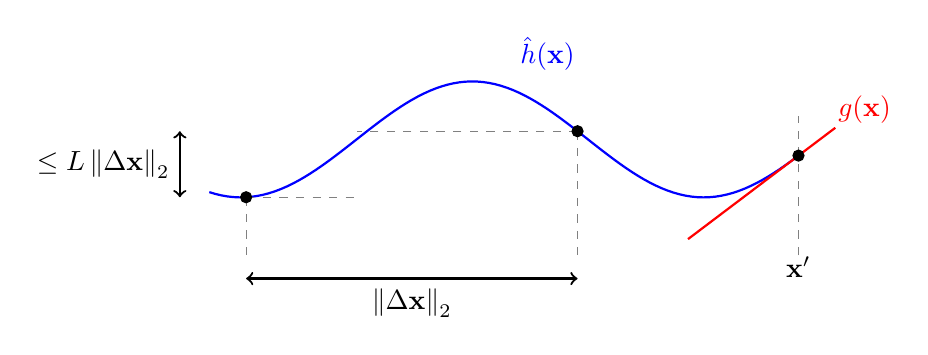
\begin{tikzpicture}[x=0.5cm]
		\begin{axis}[
			hide axis,
			xmin=-3, xmax=6,
			ymin=0, ymax=6,
			domain=0:6,
			samples=100,
			width=10cm,
			height=6cm,
			clip=false
			]
		
			\addplot[blue, thick, domain=-2:6] {2 + sin(deg(x))} 
			node[pos=0.5, above right, yshift=3pt] {$\hat{h}({\bf x})$};
		
		
			\addplot[red, thick, domain=4.5:6.5] 
			{2 + sin(deg(6)) + cos(deg(6))*(x - 6)}
			node[pos=0.95, above right] {$g({\bf x})$};
		
			\addplot[mark=*] coordinates {(6, {2 + sin(deg(6))})};
			    
			\addplot[dashed, gray] coordinates {(6,0) (6,2.4)};
			\node at (axis cs:6, -0.2) {${\bf x}'$};
			    
			    
			\pgfmathsetmacro{\xA}{-1.5}
			\pgfmathsetmacro{\xB}{3}
			\pgfmathsetmacro{\yA}{2 + sin(deg(\xA))}
			\pgfmathsetmacro{\yB}{2 + sin(deg(\xB))}
			\addplot[mark=*, only marks] coordinates {(\xA, \yA) (\xB, \yB)};
		
		
			
			\draw[dashed, gray] (axis cs:\xA,\yA) -- (axis cs:\xA,0);
			\draw[dashed, gray] (axis cs:\xB,\yB) -- (axis cs:\xB,0);
			\draw[dashed, gray] (axis cs:\xA,\yA) -- (axis cs:0,\yA);
			\draw[dashed, gray] (axis cs:\xB,\yB) -- (axis cs:0,\yB);
			 
			\draw[<->, thick] (axis cs:\xA,-0.4) -- node[below] {$\left\Vert  {\Delta {\bf x}} \right\Vert_{2}$} (axis cs:\xB,-0.4);
			
			\draw[<->, thick] (axis cs:-2.4,\yA) -- node[left] {$\leq L \left\Vert  {\Delta {\bf x}} \right\Vert_{2}$} (axis cs:-2.4,\yB);
		\end{axis}
		\vspace*{-10mm}
	\end{tikzpicture}
		\vspace*{-5mm}
	\end{center}
	\caption{
		A trained model $\hat{h}({\bf x})$ that is differentiable at a point ${\bf x}'$ 
		can be locally approximated by a linear map $g \in \mathcal{H}^{(d)}$. This local approximation 
		is determined by the gradient $\nabla \hat{h}({\bf x}')$.}
		\label{fig_linapprox_dict}
	\end{figure}
		See also: model, hypothesis space, linear map, interpretability, LIME.}, 
   first={linear model},
   plural={linear models},
   firstplural={linear models}, 
   text={linear model}
}
	
	
\newglossaryentry{gradstep}
{name={gradient step}, 
	description={Given a differentiable 
		real-valued function $f(\cdot): \mathbb{R}^{d} \rightarrow \mathbb{R}$ 
		and a vector ${\bf w} \in \mathbb{R}^{d}$, the gradient step 
		updates ${\bf w}$ by adding the scaled negative gradient $\nabla f({\bf w})$ to obtain 
		the new vector (see Fig. \ref{fig_basic_GD_step_single_dict})
		\begin{equation}
		\label{equ_def_gd_basic_dict} 
		\widehat{{\bf w}}  := {\bf w} - \eta \nabla f({\bf w}).
		\end{equation} 
		Mathematically, the gradient step is an operator $\mathcal{T}^{(f,\eta)}$ 
		that is paramet\-rized by the function $f$ and the step size $\eta$. 
		\begin{figure}[H]
			\begin{center}
				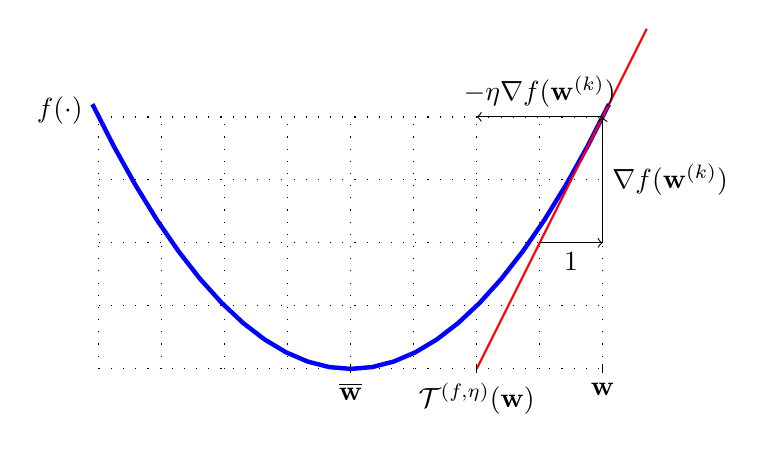
\begin{tikzpicture}[scale=0.8]
					\draw[loosely dotted] (-4,0) grid (4,4);
					\draw[blue, ultra thick, domain=-4.1:4.1] plot (\x,  {(1/4)*\x*\x});
					\draw[red, thick, domain=2:4.7] plot (\x,  {2*\x - 4});
					\draw[<-] (4,4) -- node[right] {$\nabla f({\bf w}^{(k)})$} (4,2);
					\draw[->] (4,4) -- node[above] {$-\eta \nabla f({\bf w}^{(k)})$} (2,4);
					\draw[<-] (4,2) -- node[below] {$1$} (3,2) ;
					
					\node[left] at (-4.1, 4.1) {$f(\cdot)$}; 
					\draw[shift={(0,0)}] (0pt,2pt) -- (0pt,-2pt) node[below] {$\overline{{\bf w}}$};
					\draw[shift={(4,0)}] (0pt,2pt) -- (0pt,-2pt) node[below] {${\bf w}$};
					\draw[shift={(2,0)}] (0pt,2pt) -- (0pt,-2pt) node[below] {$\mathcal{T}^{(f,\eta)}({\bf w})$};
				\end{tikzpicture}
			\end{center}
			\caption{The basic gradient step \eqref{equ_def_gd_basic_dict} maps a given vector ${\bf w}$ 
			to the updated vector ${\bf w}'$. It defines an operator 
			$\mathcal{T}^{(f,\eta)}(\cdot): \mathbb{R}^{d} \rightarrow \mathbb{R}^{d}:
			 {\bf w} \mapsto \widehat{{\bf w}}$.}
			\label{fig_basic_GD_step_single_dict}
		\end{figure}
		Note that the gradient step \eqref{equ_def_gd_basic_dict} optimizes locally—in a neighborhood whose size is 
		determined by the step size $\eta$—a linear approximation 
		to the function $f(\cdot)$. A natural generalization of \eqref{equ_def_gd_basic_dict} is to locally 
		optimize the function itself—instead of its linear approximation—such that
		\begin{align} 
		\label{equ_approx_gd_step_dict}
		\widehat{{\bf w}} = \aargmin_{{\bf w}' \in \mathbb{R}^{d}} f({\bf w}')\!+\!\frac{1}{\eta}\left\Vert  {{\bf w}-{\bf w}'} \right\Vert_{2}^2. 
		\end{align}
		We intentionally use the same symbol $\eta$ for the parameter in \eqref{equ_approx_gd_step_dict} 
		as we used for the step size in \eqref{equ_def_gd_basic_dict}. The larger the $\eta$ we choose in 
		\eqref{equ_approx_gd_step_dict}, the more progress the update will make toward reducing the 
		function value $f(\widehat{{\bf w}})$. Note that, much like the gradient step \eqref{equ_def_gd_basic_dict}, 
		the update \eqref{equ_approx_gd_step_dict} also defines an operator 
		that is parameterized by the function $f(\cdot)$ and the learning rate $\eta$. For a convex function  
		$f(\cdot)$, this operator is known as the proximal operator of $f(\cdot)$ \cite{ProximalMethods}. 
					\\ 
		See also: differentiable, function, vector, gradient, step size, neighborhood, generalization, parameter, learning rate, convex, proximal operator.},
	first={gradient step},
	firstplural={gradient steps},
	plural={gradient steps},
	text={gradient step}
}

\newglossaryentry{contractop}
{name={contraction operator},
	description={An operator $\mathcal{F}: \mathbb{R}^{d} \rightarrow \mathbb{R}^{d}$
		is a contraction if, for some $\kappa \in [0,1)$,
		\begin{equation} 
			\nonumber
			\left\Vert  { \mathcal{F} {\bf w}\!-\!\mathcal{F} {\bf w}'} \right\Vert_{2}  \leq  \kappa	\left\Vert  {{\bf w}\!-\!{\bf w}'} \right\Vert_{2} \mbox{ holds for any } {\bf w},{\bf w}' \in \mathbb{R}^{d}.
		\end{equation}
	},
	first={contraction operator},
	text={contraction operator}, 
	firstplural={contraction operators}, 
	plural={contraction operators}
}
	

\newglossaryentry{proxop}
{name={proximal operator},
	description={Given a convex 
		function $f({\bf w}')$, we define its proximal operator as \cite{Bauschke:2017}, \cite{ProximalMethods}  
		$${\rm\bf prox}_{f(\cdot),\rho}({\bf w}):= \aargmin_{{\bf w}' \in \mathbb{R}^{d}} \bigg[ f({\bf w}')\!+\!\frac{\rho}{2} \left\Vert  {{\bf w}- {\bf w}'} \right\Vert_{2}^{2}\bigg] \mbox{ with } \rho > 0. $$ 
		As illustrated in Fig. \ref{fig_proxoperator_opt_dict}, evaluating the proximal operator 
		amounts to minimizing a penalized variant of $f({\bf w}')$. The penalty term is the 
		scaled squared Euclidean distance to a given vector ${\bf w}$ (which is the input to the proximal operator). 
		The proximal operator can be interpreted as a generalization of the gradient step, which is defined 
		for a smooth convex function $f({\bf w}')$. Indeed, taking a 
		gradient step with step size $\eta$ at the current vector ${\bf w}$ 
		is the same as applying the proximal operator of the function $\tilde{f}({\bf w}')= \big( \nabla f({\bf w})\big)\,^{T} ({\bf w}'-{\bf w})$ 
		and using $\rho=1/\eta$.
			\begin{figure}[H]
			\begin{center}
				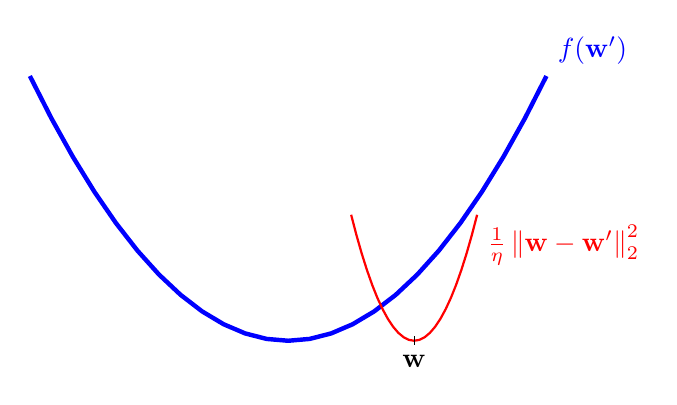
\begin{tikzpicture}[scale=0.8]
					
					\draw[blue, ultra thick, domain=-4.1:4.1] plot (\x, {(1/4)*\x*\x}) node[above right] {$f({\bf w}')$};		
					
					\draw[red, thick, domain=1:3] plot (\x, {2*(\x - 2)*(\x - 2)}) node[below right] {$\frac{1}{\eta}\left\Vert  {{\bf w}-{\bf w}'} \right\Vert_{2}^{2}$};
					
					
					\draw[shift={(2,0)}] (0pt,2pt) -- (0pt,-2pt) node[below] {${\bf w}$};
					
				\end{tikzpicture}
			\end{center}
			\caption{The proximal operator updates a vector ${\bf w}$ by minimizing a penalized version 
				of the function $f(\cdot)$. The penalty term is the scaled squared Euclidean distance between the optimization 
				variable ${\bf w}'$ and the given vector ${\bf w}$.	\label{fig_proxoperator_opt_dict}}
		\end{figure}
		See also: convex, function, vector, generalization, gradient step, smooth, step size.},
	first={proximal operator},
	text={proximal operator}
}

\newglossaryentry{proximable}
{name={proximable},
	description={A 
		convex function for which the proximal operator can be computed efficiently is 
		sometimes referred to as proximable or simple \cite{Condat2013}.
					\\ 
		See also: convex, function, proximal operator.},
	first={proximable},
	text={proximable}
}


\newglossaryentry{connected}
{name={connected graph}, 
	description={An 
		undirected graph $\mathcal{G}=\left( \mathcal{V},\mathcal{E} \right)$ is connected if every 
		non-empty subset $\mathcal{V}' \subset \mathcal{V}$ has at least one edge connecting it to $\mathcal{V} \setminus \mathcal{V}'$.
					\\ 
		See also: graph.}, 
	first={connected graph},
	text={connected graph}
}
	
	
\newglossaryentry{mvndist}
{name={multivariate normal distribution}, 
	description={The multivariate normal distribution, 
		which is denoted $\mathcal{N}\left({\bm \mu},{\bf \Sigma}\right)$, is a fundamental 
		probabilistic model for numerical feature vectors of fixed dimension $d$. 
		It defines a family of probability distributions over vector-valued RVs 
		${\bf x} \in \mathbb{R}^{d}$~\cite{BertsekasProb}, \cite{GrayProbBook}, \cite{Lapidoth09}. 
		Each distribution in this family is fully specified by its mean vector 
		${\bm \mu} \in \mathbb{R}^{d}$ and covariance matrix 
		${\bf \Sigma} \in \mathbb{R}^{d \times d}$. When the 
		covariance matrix ${\bf \Sigma}$ is invertible, the corresponding probability distribution is 
		characterized by the following pdf:
		\[p({\bf x}) = 
 		\frac{1}{\sqrt{(2\pi)^{d} \det\,({\bf \Sigma})}} 
 		\exp\left[ -\frac{1}{2} 
 		({\bf x} - {\bm \mu})\,^{T}\, {\bf \Sigma}^{-1} 
 		({\bf x} - {\bm \mu}) \right].
 		\]
		Note that this pdf is only defined when ${\bf \Sigma}$ is invertible.
   		More generally, any RV ${\bf x} \sim \mathcal{N}\left({\bm \mu},{\bf \Sigma}\right)$ 
   		admits the following representation:
  		\[
    		{\bf x} = {\bf A} {\bf z} + {\bm \mu}
   		\]
   		where ${\bf z} \sim \mathcal{N}\left(\mathbf{0},\mathbf{I}\right)$ is a standard normal vector 
   		and ${\bf A} \in \mathbb{R}^{d \times d}$ satisfies ${\bf A} {\bf A}^\top = {\bf \Sigma}$. 
   		This representation remains valid even when ${\bf \Sigma}$ is singular, in which case ${\bf A}$ 
   		is not full rank~\cite[Ch. 23]{Lapidoth2017}.
   		The family of multivariate normal distributions is exceptional among probabilistic models for numerical 
   		quantities, at least for the following reasons. First, the family is closed under affine 
   		transformations, i.e.,
		\[ 
		{\bf x} \sim \mathcal{N}({\bm \mu},{\bf \Sigma}) \mbox{ implies } 
		{\bf B}{\bf x}\!+\!{\bf c} \sim \mathcal{N}\big( {\bf B}{\bm \mu}+{\bf c},{\bf B} {\bf \Sigma} {\bf B}\,^{T} \big). 
		\]
		Second, the probability distribution $\mathcal{N}(\mathbf{0},{\bf \Sigma})$ maximizes the 
		differential entropy among all distributions with the same covariance matrix ${\bf \Sigma}$~\cite{coverthomas}. 
		\\ 
		See also: probabilistic model, probability distribution, standard normal vector, differential entropy, Gaussian RV.}, 
	first={multivariate normal distribution},
	text={multivariate normal distribution}
}

\newglossaryentry{stdnormvec}
{name={standard normal vector}, 
	description={A standard normal vector is a random 
		vector ${\bf x}=\big(x_{1}, \,\ldots, \,x_{d}\big)\,^{T}$ 
		whose entries are iid Gaussian RVs $x_{j} \sim \mathcal{N}(0,1)$. 
		It is a special case of a multivariate normal distribution, ${\bf x} \sim \mathcal(\mathbf{0},\mathbf{I})$.
		\\ 
		See also: vector, iid, Gaussian RV, multivariate normal distribution, RV.}, 
	first={standard normal vector},
	text={standard normal vector}
}

\newglossaryentry{statasp}
{name={statistical aspects}, 
	description={By statistical aspects 
		of an ML method, we refer to (properties of) the probability distribution of its output 
		under a probabilistic model for the data fed into the method.
					\\ 
		See also: ML, probability distribution, probabilistic model, data.},
	first={statistical aspects},
	text={statistical aspects}
}

\newglossaryentry{compasp}
{name={computational aspects}, 
	description={By computational 
		aspects of an ML method, we mainly refer to the computational 
		resources required for its implementation. For example, if an ML method uses iterative 
		optimization techniques to solve ERM, then its computational aspects include: 1) how 
		many arithmetic operations are needed to implement a single iteration (i.e., a gradient step); 
		and 2) how many iterations are needed to obtain useful model parameters. One important 
		example of an iterative optimization technique is GD.
					\\ 
		See also: ML, ERM, gradient step, model parameters, GD.}, 
	first={computational aspects},
	text={computational aspects}
}

\newglossaryentry{zerooneloss}
{name={$\bf 0/1$ loss},
sort={zerooneloss}, 
	description={The $0/1$ loss $L^{(0/1)}\left(\left( {\bf x},y \right),h \right)$ 
		measures the quality of a classifier $h({\bf x})$ that delivers a 
		prediction $\hat{y}$ (e.g., via thresholding \eqref{equ_def_threshold_bin_classifier_dict}) 
		for the label $y$ of a data point with features ${\bf x}$. It is equal to $0$ if 
		the prediction is correct, i.e., 
		$L^{(0/1)}\left(\left( {\bf x},y \right),h \right)=0$ when $\hat{y}=y$. It is 
		equal to $1$ if the prediction is wrong, i.e., $L^{(0/1)}\left(\left( {\bf x},y \right),h \right)=1$ 
		when $\hat{y}\neqy$.
				\\ 
		See also: loss, classifier, prediction, label, data point, feature.},
    	first={$0/1$ loss},
	text={$0/1$ loss}
}

\newglossaryentry{probability}
{name={probability}, 
	description={We assign a probability value, typically chosen in the 
		interval $[0,1]$, to each event that might occur in a random experiment  
		\cite{BillingsleyProbMeasure}, \cite{BertsekasProb}, \cite{HalmosMeasure},  \cite{KallenbergBook}.
		\\
		See also: event, random experiment. },
	first={probability},
	firstplural={probabilities},
	plural={probabilities},
	text={probability}
}
	
\newglossaryentry{underfitting}
{name={underfitting},
	description={Consider 
		an ML method that uses ERM to learn a hypothesis with the minimum empirical risk 
		on a given training set. Such a method is underfitting the training set if it is 
		not able to learn a hypothesis with a sufficiently small empirical risk on the training set. 
		If a method is underfitting, it will typically also not be able to learn a hypothesis with 
		a small risk.
					\\ 
		See also: ML, ERM, hypothesis, minimum, empirical risk, training set, risk.},
	first={underfitting},
	text={underfitting}
}

\newglossaryentry{overfitting}
{name={overfitting},
	description={Consider an 
		ML method that uses ERM to learn a hypothesis with the minimum empirical risk on 
		a given training set. Such a method is overfitting the training set if it learns 
		a hypothesis with a small empirical risk on the training set but a significantly larger loss outside the training set.
					\\ 
		See also: ERM, generalization, validation, generalization gap.},
	first={overfitting},
	text={overfitting}
}

\newglossaryentry{gdpr}
{name={general data protection regulation (GDPR)},
	description={The GDPR
			was enacted by the European Union (EU), effective from 25 May 2018 \cite{GDPR2016}. 
			It safeguards the privacy and data rights of individuals in the EU. 
			The GDPR has significant implications for how data are collected, stored, and used in ML  
			applications. Key provisions include the following:
			\begin{itemize}
				\item Data minimization principle: ML systems should only use the necessary amount of personal 
				data for their purpose.
				\item Transparency and explainability: ML systems should enable their users to 
				understand how the systems make decisions that impact the users.
				\item Data subject rights: Users should get an opportunity to access, rectify, and delete their personal data, as well as to object to automated decision-making and profiling.
				\item Accountability: Organizations must ensure robust data security and demonstrate 
				compliance through documentation and regular audits.
			\end{itemize}
		See also: data, ML, data minimization principle, transparency, explainability.}, 
	first={general data protection regulation (GDPR)},
	text={GDPR}
}
	
\newglossaryentry{gaussrv}
{name={Gaussian random variable (Gaussian RV)}, 
	plural={Gaussian RVs}, 
	description={A  standard Gaussian RV is a 
		real-valued RV $x$ with pdf \cite{BertsekasProb}, \cite{GrayProbBook}, \cite{papoulis}
		\begin{equation}
			\nonumber
			p(x) = \frac{1}{\sqrt{2\pi}} \exp\,(-x^2/2). 
		\end{equation}
		Given a standard Gaussian RV $x$, we can construct a general Gaussian RV $x'$ with 
		mean $\mu$ and variance $\sigma^2$ via $x' := \sigma x + \mu$. The probability distribution of a 
		Gaussian RV is referred to as normal distribution, denoted $\mathcal{N}(\mu, \sigma^2)$. 
		\\ 
		A Gaussian random vector ${\bf x} \in \mathbb{R}^{d}$ with 
		covariance matrix $\mathbf{C}$ and mean ${\bm \mu}$ can be constructed as \cite{GrayProbBook}, \cite{papoulis}, \cite{Lapidoth09}
		\[
		{\bf x} := \mathbf{A} {\bf z} + {\bm \mu}
		\]
		where ${\bf z} := \big( z_{1}, \,\ldots, \,z_{d} \big)\,^{T}$ is a vector 
		of iid standard Gaussian RVs, and ${\bf A} \in \mathbb{R}^{d \times d}$ is any matrix satisfying ${\bf A} {\bf A}\,^{T} = {\bf C}$. 
		The probability distribution of a Gaussian random vector is referred to as the multivariate normal distribution, 
		denoted $\mathcal{N}({\bm \mu}, \mathbf{C})$.
		\\
		We can interpret a Gaussian random vector ${\bf x}=\big(x_{1},\,\ldots,\,x_{d}\big)$ as a stochastic process 
		indexed by the set $\mathcal{I}=\{1,\,\ldots,\,d\}$. A GPs is a 
		stochastic process over an arbitray index set $\mathcal{I}$ such that any restriction to a finite subset 
		$\mathcal{I}' \subseteq \mathcal{I}$ yields a Gaussian random vector \cite{Rasmussen2006Gaussian}.
  		\\
        		Gaussian RVs are widely used probabilistic models in the statistical analysis of 
        		ML methods. Their significance arises partly from the CLT, which is a mathematically 
        		precise formulation of the following rule of thumb: The average of many independent RVs 
		(not necessarily Gaussian themselves) tends toward a Gaussian RV \cite{ross2013first}.
		\\ 
		The multivariate normal distribution is also distinct in that it represents maximum uncertainty. 
		Among all vector-valued RVs with a given covariance matrix ${\bf C}$, the RV ${\bf x} \sim \mathcal{N}({\bm \mu}, \mathbf{C})$ 
		maximizes differential entropy \cite[Th. 8.6.5]{coverthomas}. This makes GPs a 
		natural choice for capturing uncertainty (or lack of knowledge) in the absence of additional 
		structural information.
		\\ 
		See also: multivariate normal distribution, GP, probabilistic model, CLT, differential entropy.},
	first={Gaussian random variable (Gaussian RV)},
	text={Gaussian RV}
}
	
\newglossaryentry{clt}
{name={central limit theorem (CLT)},
	description={Consider a sequence of iid RVs \( x^{(r)} \), for \( r = 1, \,2, \,\ldots \), 
		each with mean zero and finite variance \( \sigma^2 > 0 \). 
		The  CLT states that the normalized sum 
		\[
		s^{(m)} := \frac{1}{\sqrt{m}} \sum_{r = 1}^{m} x^{(r)} 
		\]
		converges in distribution to a Gaussian RV with mean zero and variance \( \sigma^2 \) as \( m \to \infty \) \cite[Proposition~2.17]{AsympVanderVaartBook}.
		One elegant way to derive the CLT is via the characteristic function of the normalized sum \( s^{(m)} \). 
		Let $ \phi(t) = \mathbb{E}  \big\{ \exp \big( j t x \big) \big\}$ (with the imaginary unit $j = \sqrt{-1}$) 
		be the common characteristic function of each sum and $x^{(r)}$, and let \( \phi^{(m)}(t) \) 
		denote the characteristic function of \( s^{(m)} \). Define an operator \( \mathcal{T} \) acting on characteristic functions 
		such that
		\[
		\phi^{(m)}(t) = \mathcal{T}(\phi^{(m-1)})(t) := \phi\left( \frac{t}{\sqrt{m}} \right) \cdot \phi^{(m-1)}\left( \frac{\sqrt{m-1}}{\sqrt{m}} t \right).
		\]
		This fixed-point iteration captures the effect of recursively adding an iid RV ${\bf x}^{(m)}$ 
		and rescaling. Iteratively applying \( \mathcal{T} \) leads to convergence of \( \phi^{(m)}(t) \) toward the fixed point
		\[
		\phi^*(t) = \exp\,(-t^2 \sigma^2 / 2)
		\]
		which is the characteristic function of a Gaussian RV with mean zero and variance 
		\( \sigma^2 \). Generalizations of the CLT allow for dependent or nonidentically distributed RVs \cite[Sec.~2.8]{AsympVanderVaartBook}.
		\begin{figure}[H]
			\centering
			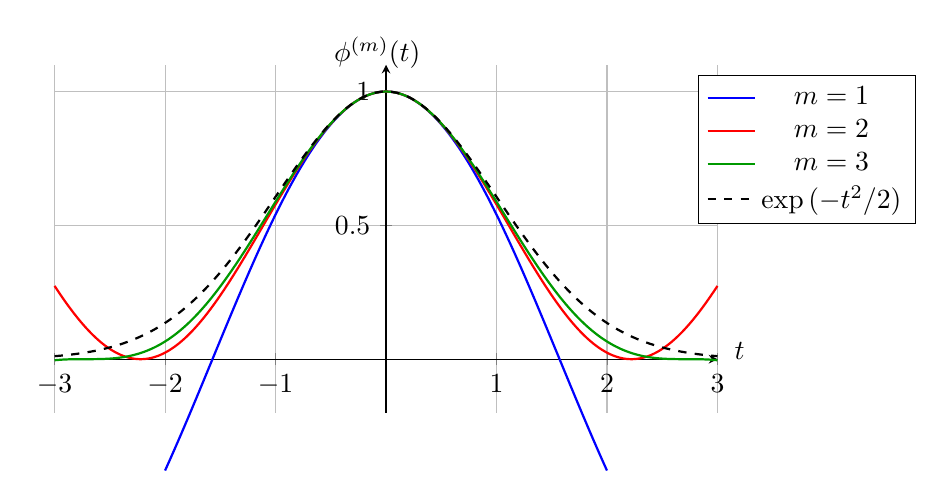
\begin{tikzpicture}
			\begin{axis}[
			width=10cm,
			height=6cm,
			xlabel={},
			ylabel={},
			legend style={at={(0.97,0.97)}, anchor=north west},
			domain=-3:3,
			ylabel style={
			yshift=10pt   
			},
			samples=400,
			ymin=-0.2, ymax=1.1,
			axis lines=middle,
			clip=false,
			grid=both,
			]
			\addplot[thick, blue,domain=-2:2] {cos(x/sqrt(1) r)^1};
			\addlegendentry{$m=1$}
			\addplot[thick, red] {cos(x/sqrt(2) r)^2};
			\addlegendentry{$m=2$}
			\addplot[thick, green!60!black] {cos(x/sqrt(3) r)^3};
			\addlegendentry{$m=3$}
			\addplot[thick, dashed, black] {exp(-x^2/2)};
			\addlegendentry{$\exp\,(-t^2/2)$}
			\node[anchor=south, rotate=0] at (axis cs:-0.08,1.05) {$\phi^{(m)}(t)$};
			\node[anchor=north, rotate=0] at (axis cs: 3.2,0.1) {$t$};
			\end{axis}
			\end{tikzpicture}
			\caption{Characteristic functions of normalized sums of iid RVs $x^{(r)} \in \{-1,1\}$ 
			for $r=1,\,\ldots,\,m$ compared to the Gaussian limit.}
		\end{figure}
		See also: RV, Gaussian RV.},
	first={central limit theorem (CLT)},
	text={CLT}
}


\newglossaryentry{GaussProc}
{name={Gaussian process (GP)},
  description={A GP is a collection of RVs 
  	$\{f({\bf x})\}_{{\bf x} \in \mathcal{X}}$ indexed by input values ${\bf x}$ 
  	from some input space $\mathcal{X}$ such that, for any finite subset 
  	${\bf x}^{(1)}, \,\ldots, \,{\bf x}^{(m)} \in \mathcal{X}$, 
  	the corresponding RVs $f({\bf x}^{(1)}, \,\ldots, \,{\bf x}^{(m)})$ 
	have a joint multivariate normal distribution 
  	\[
  	f \left( {\bf x}^{(1)}, \,\ldots, \,{\bf x}^{(m)} \right) \sim \mathcal{N}(\boldsymbol{\mu}, \mathbf{K}).
  	\]
  	For a fixed input space $\mathcal{X}$, a GP is fully specified (or parameterized) by: 1) a mean function $\mu({\bf x}) = \mathbb{E} \{ f({\bf x})\}$;
  	and 2) a covariance function $K\big({\bf x},{\bf x}'\big)= \mathbb{E} \{ \big(f({\bf x})-\mu({\bf x})\big) \big(f({\bf x}')-\mu({\bf x}')\big) \big\}$.\\
  	Example: We can interpret the temperature distribution across Finland (at a specific 
  	point in time) as the realization of a GP $f({\bf x})$, where each input ${\bf x} = (\text{lat}, \text{lon})$ 
  	denotes a geographic location. Temperature observations from FMI weather stations provide 
  	samples of $f({\bf x})$ at specific locations (see Fig. \ref{fig_gp_FMI_dict}). A GP allows us to 
  	predict the temperature nearby FMI weather stations and to quantify the uncertainty 
  	of these predictions. 
  	\begin{figure}[H]
  	\begin{center}
  		\begin{tikzpicture}
		\begin{axis}[
		axis equal,
		hide axis,
		scale=1.2,
		xmin=17, xmax=32,
		ymin=55, ymax=71,
		
		
		clip=true
		]
		
		\addplot[
		color=black,
		thick
		] table [x=lon, y=lat, col sep=comma] {assets/finland_border.csv};
		
		\addplot[
		only marks,
		mark=*,
		mark options={fill=blue},
		color=black
		] table [x=lon, y=lat, col sep=comma] {assets/fmi_stations_subset.csv};
		
		\draw[->, thick] (axis cs:19,59) -- (axis cs:25.5,59) node[anchor=west] {lon};
		\draw[->, thick] (axis cs:19,59) -- (axis cs:19,65.5) node[anchor=south] {lat};
		\end{axis}
		\end{tikzpicture}
		\vspace*{-15mm}
	\end{center}
	\caption{For a given point in time, we can interpret the current temperature distribution 
	over Finland as a realization of a GP indexed by geographic coordinates and 
	sampled at FMI weather stations. The weather stations are indicated by blue dots. \label{fig_gp_FMI_dict}}
	\end{figure}
	See also: multivariate normal distribution, uncertainty, Gaussian RV.}, 
  first={GP}, 
  text={GP}
}

\newglossaryentry{trustAI}
{name={trustworthy artificial intelligence (trustworthy AI)},
	description={Besides the computational aspects and statistical aspects, a third main design aspect of 
		ML methods is their trustworthiness \cite{pfau2024engineeringtrustworthyaideveloper}. 
		The EU has put forward seven key requirements (KRs) for trustworthy 
		AI (that typically build on ML methods) \cite{ALTAIEU}: 
	\begin{enumerate}[label=\arabic*)]
		\item KR1 – Human agency and oversight;
		\item KR2 – Technical robustness and safety;
		\item KR3 – Privacy and data governance;
		\item KR4 – Transparency;
		\item KR5 – Diversity, non-discrimination and fairness; 
		\item KR6 – Societal and environmental well-being;
		\item KR7 – Accountability. 
	\end{enumerate}
		See also: computational aspects, statistical aspects, ML, AI, robustness, data, transparency.},
	first={trustworthy artificial intelligence (trustworthy AI)},
	text={trustworthy AI}
}

\newglossaryentry{sqerrloss}
{name={squared error loss},
	description={The squared 
		error loss measures the prediction error of a 
		hypothesis $h$ when predicting a numeric label $y \in \mathbb{R}$ 
		from the features ${\bf x}$ of a data point. It is defined as 
		\begin{equation} 
			\nonumber
			L\left(({\bf x},y),h \right) := \big(y - \underbrace{h({\bf x})}_{=\hat{y}} \big)^{2}. 
		\end{equation} 
			\\ 
		See also: loss, prediction, hypothesis, label, feature, data point.},
	first={squared error loss},
	text={squared error loss}
}


 \newglossaryentry{projection}
 {name={projection}, 
       description={Consider a subset $\mathcal{W} \subseteq \mathbb{R}^{d}$ of 
	   the $d$-dimensional Euclidean space. We define the projection $P_{\mathcal{W}}\big( {\bf w}\big) $
	   of a vector ${\bf w} \in \mathbb{R}^{d}$ onto $\mathcal{W}$ as
	   \begin{equation} 
   	   	\nonumber
		\label{equ_def_proj_generic_dict}
  	    	P_{\mathcal{W}}\big( {\bf w}\big)  = \aargmin_{{\bf w}' \in \mathcal{W}} \left\Vert  {{\bf w} - {\bf w}'} \right\Vert_{2}. 
        	    \end{equation}
	    In other words, $P_{\mathcal{W}}\big( {\bf w}\big) $ is the vector in $\mathcal{W}$ 
	    that is closest to ${\bf w}$. The projection is only well defined for subsets $\mathcal{W}$ 
	    for which the above minimum exists \cite{BoydConvexBook}.
		 			\\ 
	    See also: Euclidean space, vector, minimum.},
	first={projection},
	text={projection}
}


\newglossaryentry{projgd}
{name={projected gradient descent (projected GD)},
description={Consider an ERM-based method that uses a parameterized model with  
parameter space $\mathcal{W} \subseteq \mathbb{R}^{d}$. Even if 
the objective function of ERM is smooth, we cannot use basic GD, as 
it does not take into account contraints on the optimization variable (i.e., the model parameters). 
Projected GD 
extends basic GD to handle constraints on the optimization variable (i.e., the model parameters). 
A single iteration of projected GD consists of first taking a gradient step 
and then projecting the result back onto the parameter space.
\begin{figure}[H]
	\begin{center}
		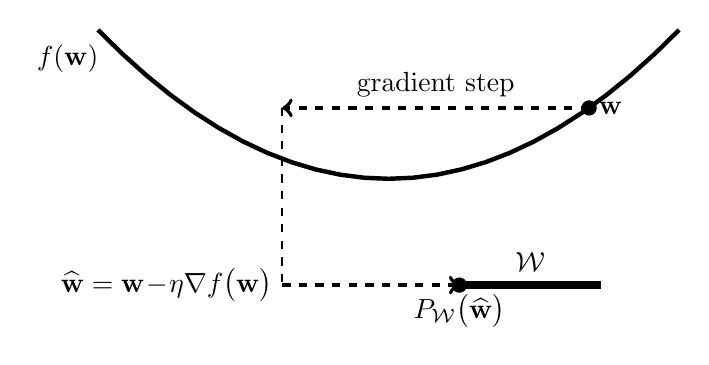
\begin{tikzpicture}[scale=0.9]
			\node [right] at (-5.1,1.7) {$f({\bf w})$} ;
			\draw[ultra thick, domain=-4.1:4.1] plot (\x,  {(1/8)*\x*\x});
		
			\draw [fill] (2.83,1) circle [radius=0.1] node[right] {${\bf w}$};
			\draw[line width =0.5mm,dashed,->] (2.83,1) -- node[midway,above] {gradient step} (-1.5,1);
			\draw[line width =0.2mm,dashed] (-1.5,1) --(-1.5,-1.5)  node [below, left]{$\widehat{{\bf w}}={\bf w}\!-\!\eta \nabla f\big({\bf w}\big)$} ;
			\draw[line width =0.5mm,dashed,->] (-1.5,-1.5)  -- node[midway,above] {} (1,-1.5) ; 
			\draw [fill] (1,-1.5) circle [radius=0.1] node[below] {$P_{\mathcal{W}}\big( \widehat{{\bf w}}\big) $};
			\draw[line width=1mm] (1,-1.5) -- (3,-1.5) node[midway, above] {$\mathcal{W}$};
		\end{tikzpicture}
		\vspace*{-5mm}
	\end{center}
	\caption{Projected GD augments a basic gradient step with a projection back 
	onto the constraint set $\mathcal{W}$.}
	\label{fig_projected_GD_dict}
\end{figure}
		See also: ERM, model, parameter space, objective function, smooth, GD, model parameters, gradient step, projection.},
	first={projected gradient descent (projected GD)},
	text={projected GD}
}

\newglossaryentry{diffpriv}
{name={differential privacy (DP)},
  description={Consider some ML method $\mathcal{A}$ 
  	that reads in a dataset (e.g., the training set 
  	used for ERM) and delivers some output $\mathcal{A}(\mathcal{D})$. The output 
  	could be either the learned model parameters or the predictions for specific data points. 
  	DP is a precise measure of privacy leakage incurred by revealing the 
  	output. Roughly speaking, an ML method is differentially private if the probability distribution 
  	of the output $\mathcal{A}(\mathcal{D})$ remains largely unchanged if the sensitive attribute 
  	of one data point in the training set is changed. Note that DP 
  	builds on a probabilistic model for an ML method, i.e., we interpret its output $\mathcal{A}(\mathcal{D})$ 
  	as the realization of an RV. The randomness in the output can be ensured 
  	by intentionally adding the realization of an auxiliary RV (i.e., adding noise) to 
  	the output of the ML method.
				\\ 
	See also: privacy leakage, sensitive attribute, privacy attack, privacy funnel.}, 
  first={DP}, 
  text={DP} 
}

\newglossaryentry{robustness}
{name={robustness},
	description={Robustness is a key requirement for trustworthy AI. It
		refers to the property of an ML system to maintain acceptable performance even when 
		subjected to different forms of perturbations. These perturbations can be to the features 
		of a data point in order to manipulate the prediction delivered by a trained ML model. 
		Robustness also includes the stability of ERM-based methods against perturbations 
		of the training set. Such perturbations can occur within data poisoning attacks. 
		\\ 
		See also: trustworthy AI, ML, feature, data point, prediction, model, stability, ERM, training set, data poisoning, attack.}, 
	first={robustness}, 
	text={robustness} 
}


\newglossaryentry{stability}
{name={stability},
	description={Stability is a desirable property of an ML method $\mathcal{A}$ that maps a 
		dataset $\mathcal{D}$ (e.g., a training set) to an output $\mathcal{A}(\mathcal{D})$. The output 
		$\mathcal{A}(\mathcal{D})$ can be the learned model parameters or the prediction delivered 
		by the trained model for a specific data point. Intuitively, $\mathcal{A}$ is 
		stable if small changes in the input dataset $\mathcal{D}$ lead to small changes in the 
		output $\mathcal{A}(\mathcal{D})$. Several formal notions of stability exist that enable bounds 
		on the generalization error or risk of the method (see \cite[Ch.~13]{ShalevMLBook}).
		To build intuition, consider the three datasets depicted in Fig. \ref{fig_three_data_stability_dict}, each 
		of which is equally likely under the same data-generating probability distribution. Since the 
		optimal model parameters are determined by this underlying probability distribution, an accurate 
		ML method $\mathcal{A}$ should return the same (or very similar) output $\mathcal{A}(\mathcal{D})$ 
		for all three datasets. In other words, any useful $\mathcal{A}$ must be robust to 
		variability in sample realizations from the same probability distribution, i.e., it must be stable. 
		\begin{figure}[H]
			\centering
			\begin{tikzpicture}
				\begin{axis}[
				
				    axis lines=none,
					xlabel={$r$},
					ylabel={},
					legend pos=north west,
					ymin=0, ymax=10,
					xtick={1,2,3,4,5},
				
					grid style=dashed,
					every axis plot/.append style={very thick}
					]
					
					\addplot+[only marks,mark=*] coordinates {
						(1,2) (2,4) (3,3) (4,5) (5,7)
					};
				
					
					\addplot+[only marks,mark=square*] coordinates {
						(1,3) (2,2) (3,6) (4,4) (5,5)
					};
				
					
					\addplot+[only marks,mark=triangle*] coordinates {
						(1,5) (2,7) (3,4) (4,6) (5,3)
					};
				
				\end{axis}
			\end{tikzpicture}
			\caption{Three datasets $\mathcal{D}^{(*)}$, $\mathcal{D}^{(\square)}$, and $\mathcal{D}^{(\triangle)}$, 
				each sampled independently from the same data-generating probability distribution. A stable ML 
				method should return similar outputs when trained on any of these datasets. \label{fig_three_data_stability_dict}}
		\end{figure}
		See also: ML, dataset, training set, model parameters, prediction, model, data point, generalization, risk, data, probability distribution, sample, realization.}, 
	first={stability}, 
	text={stability} 
}

\newglossaryentry{privprot}
{name={privacy protection},
     description={Consider some ML method $\mathcal{A}$ that reads 
	 	in a dataset $\mathcal{D}$ and delivers some output $\mathcal{A}(\mathcal{D})$. The output 
	 	could be the learned model parameters $\widehat{{\bf w}}$ or the prediction 
	 	$\hat{h}({\bf x})$ obtained for a specific data point with features 
	 	${\bf x}$. Many important ML applications involve data points 
		representing humans. Each data point is characterized by features ${\bf x}$, 
		potentially a label $y$, and a sensitive attribute $s$ (e.g., a recent medical diagnosis). 
		Roughly speaking, privacy protection means that it should be impossible to infer, from the output $\mathcal{A}(\mathcal{D})$, 
		any of the sensitive attributes of data points in $\mathcal{D}$. Mathematically, privacy protection requires non-invertibility 
		of the map $\mathcal{A}(\mathcal{D})$. In general, just making $\mathcal{A}(\mathcal{D})$ non-invertible 
		is typically insufficient for privacy protection. We need to make $\mathcal{A}(\mathcal{D})$ sufficiently non-invertible. 
					\\ 
		See also: ML, dataset, model parameters, prediction, data point, feature, label, sensitive attribute, map.}, 
	first={privacy protection}, 
	text={privacy protection} 
}

\newglossaryentry{privleakage}
{name={privacy leakage},
	description={Consider an ML application that processes a 
		dataset $\mathcal{D}$ and delivers some output, such as the predictions 
		obtained for new data points. Privacy leakage arises 
		if the output carries information about a private (or sensitive) feature of 
		a data point (which might be a human) of $\mathcal{D}$. Based on a probabilistic model 
		for the data generation, we can measure the privacy leakage via the MI 
		between the output and the sensitive feature. Another quantitative measure of privacy leakage 
		is DP. The relations between different measures of privacy leakage have been 
		studied in the literature (see \cite{InfThDiffPriv}). 
				\\ 
		See also: MI, DP, privacy attack, GDPR. }, 
	first={privacy leakage}, 
	text={privacy leakage} 
}


\newglossaryentry{probmodel}
{name={probabilistic model}, plural={probabilistic models},
	description={A probabilistic model interprets data points 
		as realizations of RVs with a joint probability distribution. This joint probability distribution typically 
		involves parameters that have to be manually chosen or learned via statistical inference 
		methods such as maximum likelihood estimation \cite{LC}.
					\\ 
		See also: model, data point, realization, RV, probability distribution, parameter, maximum likelihood. }, 
	first={probabilistic model}, 
	text={probabilistic model} 
}


\newglossaryentry{mean}
{name={mean}, plural={means},
	description={The  mean of an RV ${\bf x}$, which takes 
 		on values in a Euclidean space $\mathbb{R}^{d}$, is its 
 		expectation $\mathbb{E} \{{\bf x}\}$. It is defined as the Lebesgue 
 		integral of ${\bf x}$ with respect to the underlying probability distribution $P$ (e.g., 
		see \cite{RudinBookPrinciplesMatheAnalysis} or \cite{BillingsleyProbMeasure}), i.e.,
		\[
			\mathbb{E} \{{\bf x}\} = \int_{\mathbb{R}^{d}} {\bf x} \, \mathrm{d}P({\bf x}).
		\] 
		It is useful to think of the mean as the solution of the following risk 
		minimization problem \cite{BertsekasProb}:
		\[
			\mathbb{E} \{{\bf x}\} = \aargmin_{{\bf c} \in \mathbb{R}^{d}} 
			\mathbb{E}  \big\{\left\Vert  {{\bf x} - {\bf c}} \right\Vert_{2}^{2}\big \}.
		\] 
		We also use the term to refer to the average of a finite sequence 
		${\bf x}^{(1)}, \,\ldots, \,{\bf x}^{(m)} \in \mathbb{R}^{d}$. However, 
		these two definitions are essentially the same. Indeed, we can use the sequence 
		${\bf x}^{(1)}, \,\ldots, \,{\bf x}^{(m)} \in \mathbb{R}^{d}$ to construct a 
		discrete RV $\widetilde{{\bf x}}={\bf x}^{(I)}$, with the index $I$ being chosen uniformly 
		at random from the set $\{1, \,\ldots, \,m\}$. The mean of $\widetilde{{\bf x}}$ is 
		precisely the average $({1}/{m}) \sum_{r=1}^{m} {\bf x}^{(r)}$.
			\\ 
		See also: RV, expectation, probability distribution.}, 
	first={mean}, 
	text={mean} 
}

\newglossaryentry{median}
{name={median}, 
plural={medians},
	description={A median $\mathrm{med}\,(x)$ of a real-valued RV $x$ 
 		is any number $m \in \mathbb{R}$ such that $\mathbb{P}({ x \leq m}) \geq 1/2$ and $\mathbb{P}({ x \geq m}) \geq 1/2$ \cite{LC}. 
 		\begin{figure}[H]
			\begin{center}
			\begin{tikzpicture}
 			\begin{axis}[
    			axis lines=middle,
    			xlabel={$m$},
    			ylabel={},
    			ymin=0, ymax=1.1,
    			xmin=-2, xmax=6,
    			xtick=\empty,
    			ytick={0,1/2,1},
    			domain=-2:6,
    			samples=200,
    			width=10cm,
    			height=6cm,
    			smooth,
    			enlargelimits=true,
    			clip=false
  			]
    			
			\addplot[thick, blue, name path=cdf] {1/(1 + exp(-(x - 1)))} node[pos=0.5, above, yshift=15pt] {$\mathbb{P}({x \leq m})$};    
    			\draw[dashed, gray] (axis cs:1,0) -- (axis cs:1,0.5); 
    			\draw[dashed, gray] (axis cs:-2,0.5) -- (axis cs:1,0.5); 
    			
   			\filldraw[red] (axis cs:1,0.5) circle (2pt);
  			
    			
  			\end{axis}
			\end{tikzpicture} 
			\end{center}
			\caption{A representation of a median.}
 		\end{figure}  
 		We can define the median $\mathrm{med}\,(\mathcal{D})$ 
 		of a dataset $\mathcal{D} = \{ x^{(1)}, \,\ldots, \,x^{(m)} \in \mathbb{R} \}$ 
 		via a specific RV $\tilde{x}$ that is naturally associated with $\mathcal{D}$. 
 		In particular, this RV is constructed by $\tilde{x} = x^{(I)}$, with the index $I$ 
 		being chosen uniformly at random from the set $\{1, \,\ldots, \,m\}$, i.e., $\mathbb{P}({I = r})=1/m$ for 
 		all $r=1, \,\ldots, \,m$. If the RV $x$ is integrable, a median of $x$ 
 		is the solution of the following optimization problem: 
 		$$\min_{x' \in \mathbb{R}} \mathbb{E} {|x - x'|}.$$ 
 		Like the mean, the median of a dataset $\mathcal{D}$ can also be used 
 		to estimate parameters of an underlying probabilistic model. Compared 
 		to the mean, the median is more robust to outliers. For example, 
 		a median of a dataset $\mathcal{D}$ with more than one data point does not 
 		change even if we arbitrarily increase the largest element of $\mathcal{D}$. In contrast, 
 		the mean will increase arbitrarily.
		\begin{figure}[H]
		\centering
		\begin{tikzpicture}[scale=0.7, y=0.5cm, x=0.5cm]
			\begin{scope}
				\foreach \x/\y in {
					1/2, 4/3, 7/4
				} {
					\draw[dashed, gray] (\x, 0) -- (\x, \y);
					\filldraw[blue] (\x, \y) circle (2pt);
					\node[circle, inner sep=0pt] (ptA\x) at (\x, \y) {};
				}
				\draw[dashed, thick, darkgreen] (0.5, 3) -- (10.5, 3) node[right] {$\mathrm{med}\,(\mathcal{D})$};
				\node at (7.5, -4) {(a)};
			\end{scope}
			\begin{scope}[xshift=10cm]
				\foreach \x/\y in {
					1/2, 4/3, 7/10
				} {
					\draw[dashed, gray] (\x, 0) -- (\x, \y);
					\filldraw[blue] (\x, \y) circle (2pt);
					\node[circle, inner sep=0pt] (ptB\x) at (\x, \y) {};
				}
				\draw[dashed, thick, darkgreen] (0.5, 3) -- (10.5, 3) node[right] {$\mathrm{med}\,\big(\widetilde{\mathcal{D}}\big)$};
				\node[above right=2pt and 2pt, red] at (ptB7) {outlier};
				\node at (7.5, -4) {(b)};
			\end{scope}
		\end{tikzpicture}
		\caption{The median is robust against outlier contamination. (a) Original dataset $\mathcal{D}$. (b) Noisy 
		dataset $\widetilde{\mathcal{D}}$ including an outlier.}
		\end{figure}
		See also: mean, outlier, robustness.}, 
	first={median}, 
	text={median} 
}

\newglossaryentry{variance}
{name={variance},
	description={The variance of a real-valued RV $x$ is defined as the expectation 
		$\mathbb{E} \big\{ \big( x - \mathbb{E} \{x \} \big)^{2} \big\}$ of the squared difference between $x$ 
		and its expectation $\mathbb{E} \{x \}$. We extend this definition to vector-valued RVs ${\bf x}$ 
		as $\mathbb{E} \big\{ \big\| {\bf x} - \mathbb{E} \{{\bf x} \} \big\|_{2}^{2} \big\}$.
					\\ 
		See also: RV, expectation, vector.},
	first={variance},
	text={variance} 
}

\newglossaryentry{nn}
{name={nearest neighbor (NN)},
	description={NN methods learn a hypothesis 
		$h: \mathcal{X} \rightarrow \mathcal{Y}$ whose function value $h({\bf x})$ 
		is solely determined by the NNs within a given dataset. Different 
		methods use different metrics for determining the NNs. If data points 
		are characterized by numeric feature vectors, we can use their Euclidean distances as 
		the metric.
					\\ 
		See also: hypothesis, function, dataset, metric, data point, feature vector, neighbors.},
	first={nearest neighbor (NN)},
	text={NN} 
}

\newglossaryentry{neighborhood}
{name={neighborhood},
	description={The neighborhood of a node $i \in \mathcal{V}$ is 
		the subset of nodes constituted by the neighbors of $i$.
				\\ 
		See also: neighbors.},
	first={neighborhood},
	text={neighborhood} 
}


\newglossaryentry{neighbors}
{name={neighbors},
	description={The neighbors of a node $i \in \mathcal{V}$ 
		within an FL network are those nodes $i' \in \mathcal{V} \setminus \{ i\}$ that are connected (via an edge) to node $i$.
				\\ 
		See also: FL network.},
	first={neighbors},
	text={neighbors} 
}

\newglossaryentry{bias}
{name={bias},
	description={Consider an ML method using a parameterized hypothesis space $\mathcal{H}$. 
		It learns the model parameters ${\bf w} \in \mathbb{R}^{d}$ using the dataset $$\mathcal{D}=\big\{ \left( {\bf x}^{(r)},y^{(r)} \right) \big\}_{r=1}^{m}.$$ 
		To analyze the properties of the ML method, we typically interpret the data points as realizations 
		of iid RVs, $$y^{(r)} = h^{(\overline{{\bf w}})}\big( {\bf x}^{(r)} \big) + \bm{\varepsilon}^{(r)}, r=1, \,\ldots, \,m.$$ 
		We can then interpret the ML method as an estimator $\widehat{{\bf w}}$ 
		computed from $\mathcal{D}$ (e.g., by solving ERM). The (squared) bias incurred by the estimate $\widehat{{\bf w}}$ 
		is then defined as $B^{2} := \big\| \mathbb{E}  \{ \widehat{{\bf w}}  \}- \overline{{\bf w}}\big\|_{2}^{2}$.
					\\ 
		See also: ML, hypothesis space, model parameters, dataset, data point, realization, iid, RV, ERM.},
	first={bias},
	text={bias} 
}

\newglossaryentry{classification}
{name={classification},
	description={Classification is the task of determining a 
 		discrete-valued label $y$ for a given data point, based solely on its 
 		features ${\bf x}$. The label $y$ belongs to a finite set, such as 
 		$y \in \{-1,1\}$ or $y \in \{1, \,\ldots, \,19\}$, and represents the 
 		category to which the corresponding data point belongs.
				\\ 
		See also: label, data point, feature.},
	first={classification},
	text={classification} 
}


\newglossaryentry{privfunnel}
{name={privacy funnel},
	description={The privacy funnel is a method for learning privacy-friendly features 
		of data points \cite{PrivacyFunnel}.
				\\ 
		See also: feature, data point.},
 	first={privacy funnel},
	text={privacy funnel} 
}


\newglossaryentry{condnr}
{name={condition number},
	description={The condition number $\kappa(\mathbf{Q}) \geq 1$ of a 
		positive definite matrix $\mathbf{Q} \in \mathbb{R}^{d \times d}$ is the ratio 
		$\alpha /\beta  $ between the largest $\alpha$ and the smallest $\beta$ eigenvalue of 
		$\mathbf{Q}$. The condition number is useful for the analysis of ML methods. 
		The computational complexity of gradient-based methods for linear regression crucially depends on the 
		condition number of the matrix $\mathbf{Q} = {\bf X} {\bf X}\,^{T}$, with the feature matrix ${\bf X}$ 
		of the training set. Thus, from a computational perspective, we prefer features of 
		data points such that $\mathbf{Q}$ has a condition number close to $1$.
					\\ 
		See also: matrix, eigenvalue, ML, gradient-based methods, linear regression, feature matrix, training set, feature, data point.},
	first={condition number},
	text={condition number} 
}

\newglossaryentry{classifier}
{name={classifier},
	description={A classifier is a hypothesis (i.e., a map) $h({\bf x})$ 
		used to predict a label taking on values from a finite label space. We might use the 
		function value $h({\bf x})$ itself as a prediction $\hat{y}$ for 
		the label. However, it is customary to use a map $h(\cdot)$ that delivers 
		a numeric quantity. The prediction is then obtained by a simple thresholding step. 
		For example, in a binary classification problem with a label space $\mathcal{Y} \in  \{ -1,1\}$, 
		we might use a real-valued hypothesis map $h({\bf x}) \in \mathbb{R}$ 
		as a classifier. A prediction $\hat{y}$ can then be obtained via thresholding,  
		 \begin{equation} 
		 	\label{equ_def_threshold_bin_classifier_dict}
		 	\hat{y} =1   \mbox{ for } h({\bf x})\!\geq\!0 \mbox{ and } 	\hat{y} =-1  \mbox{ otherwise.}
	 		\end{equation}
 		We can characterize a classifier by its decision regions $\mathcal{R}_{a}$, for 
 		every possible label value $a \in \mathcal{Y}$.
					\\ 
		See also: hypothesis, map, label, label space, function, prediction, classification, decision region. },
	first={classifier},
	text={classifier} 
}

\newglossaryentry{emprisk}
{name={empirical risk},
  description={The empirical risk $\widehat{L}\big(h|\mathcal{D}\big)$ 
  	of a hypothesis on a dataset $\mathcal{D}$ is the average loss incurred 
  	by $h$ when applied to the data points in $\mathcal{D}$.
				\\ 
		See also: risk, hypothesis, dataset, loss, data point.},
  first={empirical risk},
  text={empirical risk} 
}

\newglossaryentry{nodedegree}
{name={node degree},
	description={The degree $d^{(i)}$ of a node $i \in \mathcal{V}$ 
		in an undirected graph is the number of its neighbors, i.e., $d^{(i)} := \big|\mathcal{N}^{(i)}\big|$.
					\\ 
		See also: graph, neighbors.},
	first={node degree},
	text={node degree} 
}

\newglossaryentry{graph}
{name={graph},
	description={A graph $\mathcal{G} = \left( \mathcal{V},\mathcal{E} \right)$ is a pair that consists of 
		a node set $\mathcal{V}$ and an edge set $\mathcal{E}$. In its most general form, a graph is 
		specified by a map that assigns each edge $e \in \mathcal{E}$ a pair of nodes \cite{RockNetworks}. 
		One important family of graphs is simple undirected graphs. A simple undirected graph 
		is obtained by identifying each edge $e \in \mathcal{E}$ with two different nodes $\{i,i'\}$. 
		Weighted graphs also specify numeric weights $A_{e}$ for each 
		edge $e \in \mathcal{E}$.
					\\ 
		See also: map, weights.},
	first={graph},
	text={graph} 
}

\newglossaryentry{uncertainty}
{name={uncertainty},
	description={In the context of ML, uncertainty refers to the presence of multiple 
		plausible outcomes or explanations based on available data. For example, the 
		prediction $\hat{h}({\bf x})$ produced by a trained ML model $\hat{h}$
	 	often reflects a range of possible values for the true label of a given data point. 
	 	The broader this range, the greater the associated uncertainty. Probability theory 
	 	allows us to represent, quantify, and reason about uncertainty in a 
	 	mathematically rigorous manner.
					\\ 
		See also: probabilistic model, risk, entropy, variance. },
	first={uncertainty},
	text={uncertainty}
}

\newglossaryentry{ucb}
{name={upper confidence bound (UCB)},
	description={Consider an ML 
		application that requires selecting, at each time step $k$, an action $a_{k}$ 
		from a finite set of alternatives $\actionset$. The utility of selecting action $a_{k}$ 
		is quantified by a numeric reward signal $r^{(a_{k})}$. 
		A widely used probabilistic model for this type of sequential decision-making problem 
		is the stochastic MAB setting \cite{Bubeck2012}. In this model, 
		the reward $r^{(a)}$ is viewed as the realization of an RV 
		with unknown mean $\mu^{(a)}$. Ideally, we would always choose the 
		action with the largest expected reward $\mu^{(a)}$, but these 
		means are unknown and must be estimated from observed data. Simply 
		choosing the action with the largest estimate $\widehat{\mu}^{(a)}$ can 
		lead to suboptimal outcomes due to estimation uncertainty. The UCB strategy 
		addresses this by selecting actions not only based on their estimated means but 
		also by incorporating a term that reflects the uncertainty in these estimates—favoring 
		actions with a high-potential reward and high uncertainty. Theoretical guarantees 
		for the performance of UCB strategies, including logarithmic regret bounds, are established in \cite{Bubeck2012}.
					\\ 
		See also: ML, reward, probabilistic model, stochastic, MAB, model, realization, RV, mean, data, uncertainty, regret.},
	first={upper confidence bound (UCB)},
	text={UCB} 
}

\newglossaryentry{mab}
{name={multi-armed bandit (MAB)},
	description={An MAB  problem is a precise mathematical 
		formulation of a sequential decision-making task under uncertainty. At each 
		discrete time step $k$, a learner selects one of several possible 
		actions—called arms—from a finite set $\actionset$. Pulling arm $a$ at time 
		$k$ yields a reward $r^{(a,k)}$ that is drawn from an unknown 
		probability distribution $\mathbb{P}({r^{(a,k)}})$. We obtain different classes 
		of MAB problems by placing different restrictions on this probability distribution. In the simplest 
		setting, the probability distribution $\mathbb{P}({r^{(a,k)}})$ does not depend on $t$. 
		Given an MAB problem, the goal is to construct ML methods that maximize the cumulative 
		reward over time by strategically balancing exploration (i.e., gathering information 
		about uncertain arms) and exploitation (i.e., selecting arms known to perform well). 
		MAB problems form an important special case of RL problems \cite{Bubeck2012}, \cite{SuttonEd2}.
					\\ 
		See also: reward, regret.},
	first={MAB},
	text={MAB}
}



\newglossaryentry{optimism in the face of uncertainty}
{name={optimism in the face of uncertainty},
	description={ML methods learn model parameters ${\bf w}$ 
		according to some performance criterion $\bar{f}({\bf w})$. However, they usually 
		cannot access $\bar{f}({\bf w})$ directly but rely on an estimate (or approximation) 
		$f({\bf w})$ of $\bar{f}({\bf w})$. As a case in point, ERM-based methods use 
		the average loss on a given dataset (i.e., the training set) as an estimate 
		for the risk of a hypothesis. Using a probabilistic model, one can construct 
		a confidence interval 
		$\big[ l^{({\bf w})},  u^{({\bf w})} \big]$ for each choice ${\bf w}$ for the model parameters.
		One simple construction is $l^{({\bf w})} := f({\bf w}) - \sigma/2$, $u^{({\bf w})} := f({\bf w})+ \sigma/2$, 
	    	with $\sigma$ being a measure of the (expected) deviation of $f({\bf w})$ from $\bar{f}({\bf w})$.
		We can also use other constructions for this interval as long as they ensure that $\bar{f}({\bf w}) \in\big[ l^{({\bf w})},  u^{({\bf w})} \big]$ 
		with a sufficiently high probability. An optimist chooses the model parameters 
		according to the most favorable—yet still plausible—value $\tilde{f}({\bf w}) :=  l^{({\bf w})}$ 
		of the performance criterion. Two examples of ML methods that use such an optimistic 
		construction of an objective function are SRM \cite[Ch. 11]{ShalevMLBook} and UCB methods 
		for sequential decision making \cite[Sec. 2.2]{Bubeck2012}. 
		\begin{figure}[H]
				\begin{center}
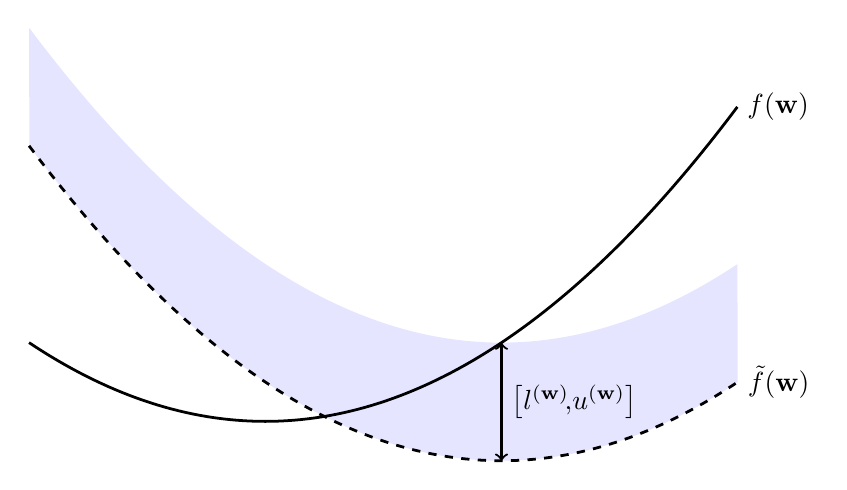
\begin{tikzpicture}[x=3cm, y=1cm]
  
\fill[blue!10] 
(-1, 5) -- plot[domain=-2:1, samples=100] ({\x+1}, {\x*\x + 1}) -- 
plot[domain=1:-2, samples=100] ({\x+1}, {\x*\x - 0.5}) -- cycle;
  \node[anchor=west] at (2, 4) {$f({\bf w})$};
  \draw[line width=1, domain=-2:1, samples=100,dashed] plot  ({\x+1}, {\x*\x -0.5}) node[right] {$\tilde{f}({\bf w})$};
   \draw[line width=1, domain=-1:2, samples=100] plot ({\x}, {\x*\x});
  \draw[<->, thick] (1, -0.5) -- (1, 1) node[midway, right] {$\big[ l^{({\bf w})}\!,\!u^{({\bf w})} \big]$};
\end{tikzpicture}
\caption{ML methods learn model parameters ${\bf w}$ by using some estimate of $f({\bf w})$ for 
	the ultimate performance criterion $\bar{f}({\bf w})$. Using a probabilistic model, one can use $f({\bf w})$ to 
	construct confidence intervals $\big[ l^{({\bf w})},  u^{({\bf w})} \big]$, which contain $\bar{f}({\bf w})$  
	with a high probability. The best plausible performance measure for a specific choice ${\bf w}$ of model parameters 
	is $\tilde{f}({\bf w}) := l^{({\bf w})}$.} 
	\end{center}
		\end{figure}
		See also: ML, model parameters, ERM, loss, dataset, training set, risk, hypothesis, probabilistic model, probability, objective function, SRM, UCB.},
	first={optimism in the face of uncertainty},
	text={optimism in the face of uncertainty} 
}

\newglossaryentry{empgraph}
{name={federated learning network (FL network)},
	description={An FL network consists of 
		an undirected weighted graph $\mathcal{G}$. The nodes of $\mathcal{G}$ represent devices 
		that can access a local dataset and train a local model. The edges of $\mathcal{G}$ represent 
		communication links between devices as well as statistical similarities between their local datasets. 
		A principled approach to train the local models is GTVMin. The solutions of GTVMin are local 
		model parameters that optimally balance the loss incurred on local datasets with their discrepancy 
		across the edges of $\mathcal{G}$.
	    			\\ 
		See also: FL, graph, device, GTVMin.},
	first={federated learning network (FL network)},
	text={FL network} 
}

\newglossaryentry{norm}
{name={norm},
	description={A norm is a function that maps each (vector) element 
		of a vector space to a nonnegative real number. This function must be 
		homogeneous and definite, and it must satisfy the triangle inequality \cite{HornMatAnalysis}.
		\\
		See also: function, vector, vector space.},
	first={norm},
	text={norm} 
}

\newglossaryentry{dualnorm}
{name={dual norm},
	description={Every norm $\left\Vert  {\cdot} \right\Vert_{}$ defined on a Euclidean space $\mathbb{R}^{d}$ 
		has an associated dual norm, which is denoted $\left\Vert  {\cdot} \right\Vert_{*}$ and defined as 
		$\left\Vert  {{\bf y}} \right\Vert_{*} := \sup_{\Vert  {{\bf x}} \Vert{} \le 1} {\bf y}\,^{T} {\bf x}$. 
		The dual norm measures the largest possible inner product between ${\bf y}$ 
		and any vector in the unit ball of the original norm. For further details, see 
		\cite[Sec.~A.1.6]{BoydConvexBook}.
					\\ 
		See also: norm, Euclidean space, vector.},
	first={dual norm},
	text={dual norm}
}

\newglossaryentry{geometricmedian}
{name={geometric median (GM)},
	description={The GM of a set of input vectors ${\bf x}^{(1)}, \,\ldots, \,{\bf x}^{(m)}$ 
		in $\mathbb{R}^{d}$ is a point ${\bf z} \in \mathbb{R}^{d}$ that 
		minimizes the sum of distances to the vectors \cite{BoydConvexBook} such that 
		\begin{equation} 
			\label{equ_geometric_median_dict}
		{\bf z} \in \aargmin_{{\bf y} \in \mathbb{R}^{d}} \sum_{r=1}^{m} \left\Vert  {{\bf y} - {\bf x}^{(r)}} \right\Vert_{2}.
		\end{equation} 
		Fig. \ref{opt_cond_GM_dict} illustrates a fundamental property of the GM:
		If ${\bf z}$ does not coincide with any of the input vectors, then the unit vectors pointing 
		from ${\bf z}$ to each ${\bf x}^{(r)}$ must sum to zero—this is the zero-subgradient  
		(optimality) condition for \eqref{equ_geometric_median_dict}. It turns out that the solution to 
		\eqref{equ_geometric_median_dict} cannot be arbitrarily pulled away from trustworthy input 
		vectors as long as they are the majority \cite[Th. 2.2]{Lopuhaae1991}.
	  	\begin{figure}[H]
  		\begin{center}
			\begin{tikzpicture}[scale=2, thick, >=stealth]

				\coordinate (w) at (3,0);
				\fill (w) circle (1.2pt) node[below right] {${\bf z}$};

				\coordinate (w2) at (0.5,0.3);
				\coordinate (w3) at (0.7,0.7);
				\fill (w2) circle (1pt) node[above left] {${\bf x}^{(1)}$};
				\fill (w3) circle (1pt) node[above left] {${\bf x}^{(2)}$};
			    \node[anchor=west] at ($(w2) +(-0.2,0.9)$) {\textbf{clean}};

				\draw[dashed] (w) -- (w2);
				\draw[dashed] (w) -- (w3);

				\draw[->, thick, red] (w) -- ($(w)!1cm!(w2)$) ;
				\draw[->, thick, red] (w) -- ($(w)!1cm!(w3)$) node[pos=0.9, right,yshift=7pt] {$\frac{{\bf x}^{(2)}- {\bf z}}{\left\Vert  {{\bf x}^{(2)}-{\bf z}} \right\Vert_{2}}$};

				\coordinate (w4) at (5,0.2);
				\node at (5,0.6) {\textbf{perturbed}};
				\fill (w4) circle (1pt) node[below left] {${\bf x}^{(3)}$};
				\draw[->, thick, red] (w) -- ($(w)!1cm!(w4)$) ;

		\end{tikzpicture}
		\caption{\label{opt_cond_GM_dict}
			Consider a solution ${\bf z}$ of \eqref{equ_geometric_median_dict} that does not coincide 
			with any of the input vectors. The optimality condition for \eqref{equ_geometric_median_dict} 
			requires that the unit vectors from ${\bf z}$ to the input vectors sum to zero.}
			\end{center}
		\end{figure}
		See also: vector, subgradient.},
	first={geometric median},
	text={GM}
}


\newglossaryentry{explanation}
{name={explanation}, plural={explanations},
	description={One approach to enhance the transparency of an ML method for its human user 
		is to provide an explanation alongside the predictions delivered 
		by the method. Explanations can take different forms. For instance, they may 
        		consist of human-readable text or quantitative indicators, such as feature 
        		importance scores for the individual features of a given data point~\cite{Molnar2019}. 
	   	Alternatively, explanations can be visual, for example, intensity maps that highlight 
	   	image regions that drive the prediction \cite{GradCamPaper}. 
       		Fig.\ \ref{fig_explanation_dict} illustrates two types of explanations. The first 
       		is a local linear approximation $g({\bf x})$ of a nonlinear trained model 
       		$\hat{h}({\bf x})$ around a specific feature vector ${\bf x}'$, 
       		as used in the method LIME. 
        		The second form of explanation depicted in the figure is a sparse set of predictions 
       		$\hat{h}({\bf x}^{(1)}), \hat{h}({\bf x}^{(2)}), \hat{h}({\bf x}^{(3)})$ 
       		at selected feature vectors, offering concrete reference points for the user. 
	 	\begin{figure}[H]
	   		\begin{center}
	 		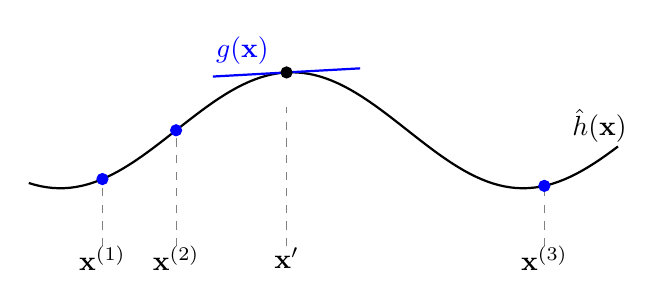
\begin{tikzpicture}[x=0.5cm]
	 		\begin{axis}[
	 			hide axis,
	 			xmin=-3, xmax=6,
	 			ymin=0, ymax=6,
	 			domain=0:6,
	 			samples=100,
	 			width=10cm,
	 			height=6cm,
	 			clip=false
	 		   ]
	 		
			\addplot[thick, domain=-2:6] {2 + sin(deg(x))} 
	   		     node[pos=0.9, above right, yshift=10pt] {$\hat{h}({\bf x})$};
	 		
	 		
	 		\addplot[blue, thick, domain=0.5:2.5] 
	 		{2 + sin(deg(1.5)) + cos(deg(1.5))*(x - 1.5)}
	 		node[pos=0.2, above] {$g({\bf x})$};
	 		
	 		\addplot[mark=*] coordinates {(1.5, {2 + sin(deg(1.5))})};
	 		    
			\addplot[dashed, gray] coordinates {(1.5,0) (1.5,2.4)};
	 		\node at (axis cs:1.5, -0.2) {${\bf x}'$};
	      		
	       		\addplot[mark=*,blue] coordinates {(-1, {2 + sin(deg(-1))})};
	       		\addplot[dashed, gray] coordinates {(-1,0) (-1,{2 + sin(deg(-1))})};
	       		\node at (axis cs:-1, -0.2) {${\bf x}^{(1)}$};
	 	   	\addplot[mark=*,blue] coordinates {(0, {2 + sin(deg(0))})};
	 	   	\addplot[dashed, gray] coordinates {(0,0) (0,{2 + sin(deg(0))})};
	 	   	\node at (axis cs:0, -0.2) {${\bf x}^{(2)}$};
	 	   	\addplot[mark=*,blue] coordinates {(5, {2 + sin(deg(5))})};
	 	   	\addplot[dashed, gray] coordinates {(5,0) (5,{2 + sin(deg(5))})};
	 	   	\node at (axis cs:5, -0.2) {${\bf x}^{(3)}$};
	
	
	
	
	
	
	 		\end{axis}
	
		\end{tikzpicture}
	 	\end{center}
	 	\caption{A trained model $\hat{h}({\bf x})$ can be explained 
	     	locally at some point ${\bf x}'$ by a linear approximation $g({\bf x})$. 
	     	For a differentiable $\hat{h}({\bf x})$, this approximation is 
	     	determined by the gradient $\nabla \hat{h}({\bf x}')$. Another 
	     	form of explanation could be the function values $\hat{h}\big({\bf x}^{(r)} \big)$ 
	     	for $r=1, 2, 3$. 
		\label{fig_explanation_dict}}
	 	\end{figure} 
		See also: ML, prediction, feature, data point, classification.},
	first={explanation},
	text={explanation} 
}

\newglossaryentry{risk}
{name={risk},
	description={Consider a hypothesis $h$ used to predict the label 
		$y$ of a data point based on its features ${\bf x}$. We measure 
		the quality of a particular prediction using a loss function $L\left(({\bf x},y),h \right)$. 
		If we interpret data points as the realizations of iid RVs, 
		the $L\left(({\bf x},y),h \right)$ also becomes the realization 
		of an RV. The i.i.d.\ assumption allows us to define the risk of a hypothesis 
		as the expected loss $\mathbb{E}  \big\{L\left(({\bf x},y),h \right) \big\}$. 
		Note that the risk of $h$ depends on both the specific choice for the loss function and the 
		probability distribution of the data points.
					\\ 
		See also: hypothesis, label, data point, feature, prediction, loss function, realization, iid RV, i.i.d.\ assumption, loss, probability distribution.},
	first={risk},
	text={risk} 
}

\newglossaryentry{actfun}
{name={activation function},
	description={Each artificial neuron within an ANN is 
		assigned an activation function $\sigma(\cdot)$ that maps a weighted combination of 
		the neuron inputs $x_{1}, \,\ldots, \,x_{d}$ to a single output 
		value $a = \sigma\big(w_{1} x_{1}+\ldots+w_{d} x_{d} \big)$. 
		Note that each neuron is parameterized by the weights $w_{1}, \,\ldots, \,w_{d}$.
					\\ 
		See also: ANN, function, weights.},
	first={activation function},
	text={activation function} 
}

\newglossaryentry{distributedalgorithm}
{name={distributed algorithm},
	description={A distributed algorithm is an algorithm designed for 
		a special type of computer, i.e., a collection of interconnected computing devices (or nodes). 
		These devices communicate and coordinate their local computations by exchanging 
		messages over a network \cite{IntroDistAlg}, \cite{ParallelDistrBook}. Unlike a classical algorithm, 
		which is implemented on a single device, a distributed algorithm is 
		executed concurrently on multiple devices with computational capabilities. 
		Similar to a classical algorithm, a distributed algorithm can be modeled as a 
		set of potential executions. However, each execution in the distributed setting involves 
		both local computations and message-passing events. A generic execution might look as 
		follows:
		\[
		\begin{array}{l}
			\text{Node 1: } {\rm input}_1, \,s_1^{(1)}, \,s_2^{(1)}, \,\ldots, \,s_{T_1}^{(1)}, \,{\rm output}_1; \\
			\text{Node 2: } {\rm input}_2, \,s_1^{(2)}, \,s_2^{(2)}, \,\ldots, \,s_{T_2}^{(2)}, \,{\rm output}_2; \\
			\quad \vdots \\
			\text{Node N: } {\rm input}_N, \,s_1^{(N)}, \,s_2^{(N)}, \,\ldots, \,s_{T_N}^{(N)}, \,{\rm output}_N.
		\end{array}
		\]
		Each device $i$ starts from its own local input and performs a sequence of 
		intermediate computations $s_{k}^{(i)}$ at discrete-time instants $k = 1, \,\dots, \,T_i$. 
		These computations may depend on both the previous local computations at the device 
		and the messages received from other devices. One important application of distributed 
		algorithms is in FL where a network of devices collaboratively trains a personal model 
		for each device. 
					\\ 
		See also: algorithm, device, event, FL, model.
		},
	first={distributed algorithm}, 
	text={distributed algorithm}
}


\newglossaryentry{algorithm}
{name={algorithm}, plural={algorithms},
 	description={An algorithm is a precise, step-by-step specification for 
  		producing an output from a given input within a finite number of computational steps \cite{Cormen:2022aa}. 
    		For example, an algorithm to train a linear model explicitly describes how to 
		transform a given training set into model parameters through a sequence of gradient steps. 
    		To study algorithms rigorously, we can represent (or approximate) them by different mathematical structures \cite{Sipser2013}. 
     		One approach is to represent an algorithm as a collection of possible executions. Each individual 
     		execution is then a sequence of the form $${\rm input}, \,s_1, \,s_2, \,\ldots, \,s_T, \,{\rm output}.$$ This sequence 
     		starts from an input and progresses via intermediate steps until an output is delivered. Crucially, an algorithm 
     		encompasses more than just a mapping from input to output; it also includes intermediate computational 
     		steps $s_1, \,\ldots, \,s_T$.
				\\ 
		See also: linear model, training set, model parameters, gradient step, model, stochastic.},
	first={algorithm},
	text={algorithm} 
}

\newglossaryentry{stochalgorithm}
{name={stochastic algorithm}, 
 plural={stochastic algorithms},
	description={A stochastic algorithm uses a random mechanism 
		during its execution. For example, SGD uses a randomly selected subset of data points 
		to compute an approximation for the gradient of an objective function. We can represent a 
		stochastic algorithm by a stochastic processes, i.e., the possible execution sequence is the possible outcomes of 
		a random experiment \cite{BertsekasProb}, \cite{RandomizedAlgos}, \cite{Gallager13}.		
		\\ 
		See also: stochastic, algorithm, SGD, data point, gradient, objective function, stochastic process, 
		random experiment, optimization method, gradient-based methods. },
	first={stochastic algorithm},
	text={stochastic algorithm} 
}

\newglossaryentry{onlinelearning}
{name={online learning},
	description={Some ML methods  are designed to process data in a sequential 
		manner, updating their model parameters one at a time, as new data points become available. 
		A typical example is time-series data, such as daily minimum and maximum temperatures 
		recorded by an FMI weather station. These values form a chronological sequence 
		of observations. During each time step $t$, online learning methods update (or refine)  
		the current hypothesis $h^{(t)}$ (or model parameters ${\bf w}^{(t)}$) 
		based on the newly observed data point ${\bf z}^{(t)}$. 
		\\ 
		See also: online GD, online algorithm. },
	first={online learning},
	text={online learning} 
}

\newglossaryentry{onlinealgorithm}
{name={online algorithm},
	description={An online algorithm processes input data incrementally, 
		receiving data points sequentially and making decisions or producing outputs (or decisions) immediately 
		without having access to the entire input in advance \cite{PredictionLearningGames}, \cite{HazanOCO}. 
		Unlike an offline algorithm, which has the entire input available from the start, an online algorithm 
		must handle uncertainty about future inputs and cannot revise past decisions. Similar to an 
		offline algorithm, we represent an online algorithm formally as a collection of possible 
		executions. However, the execution sequence for an online algorithm has a distinct structure as follows:
		$${\rm in}_{1}, \,s_1, \,{\rm out}_{1}, \,{\rm in}_{2}, \,s_2, \,{\rm out}_{2}, \,\ldots, \,{\rm in}_{T}, \,s_T, \,{\rm out}_{T}.$$ 
		Each execution begins from an initial state (i.e., \(\text{in}_{1}\)) and proceeds through alternating 
		computational steps, outputs (or decisions), and inputs. Specifically, at step \(k\), 
		the algorithm performs a computational step \(s_{k}\), generates an output \(\text{out}_{k}\), 
		and then subsequently receives the next input (data point) \(\text{in}_{k+1}\). A 
		notable example of an online algorithm in ML is online GD, which incrementally 
		updates model parameters as new data points arrive. 
					\\ 
		See also: algorithm, data, data point, uncertainty, ML, online GD, model parameters, online learning.},
	first={online algorithm},
	text={online algorithm} 
}


\newglossaryentry{transparency}
{name={transparency},
	description={Transparency is a fundamental requirement for 
		trustworthy AI \cite{HLEGTrustworhtyAI}. In the context of ML 
		methods, transparency is often used interchangeably with explainability 
		\cite{JunXML2020}, \cite{gallese2023ai}. However, in the broader scope of AI 
		systems, transparency extends beyond explainability and includes providing information 
		about the system’s limitations, reliability, and intended use. 
		In medical diagnosis systems, transparency requires disclosing the confidence level 
		for the predictions delivered by a trained model. In credit scoring, 
		AI-based lending decisions should be accompanied by explanations of 
		contributing factors, such as income level or credit history. These explanations 
		allow humans (e.g., a loan applicant) to understand and contest automated decisions. 
		Some ML methods inherently offer transparency. For example, logistic regression 
		provides a quantitative measure of classification reliability through the value $|h({\bf x})|$. 
		Decision trees are another example, as they allow human-readable decision rules \cite{rudin2019stop}.
		Transparency also requires a clear indication when a user is engaging with an AI system. 
		For example, AI-powered chatbots should notify users that they are interacting with an 
		automated system rather than a human. Furthermore, transparency encompasses comprehensive 
		documentation detailing the purpose and design choices underlying the AI system. 
		For instance, model datasheets \cite{DatasheetData2021} and AI system cards \cite{10.1145/3287560.3287596} 
		help practitioners understand the intended use cases and limitations of an AI system \cite{Shahriari2017}.
					\\ 
		See also: trustworthy AI, explainability.},
	first={transparency}, 
	text={transparency} 
}



\newglossaryentry{sensattr}
{name={sensitive attribute}, plural={sensitive attributes},
	description={ML revolves around learning a hypothesis map that allows 
		us to predict the label of a data point from its features. In some 
		applications, we must ensure that the output delivered by an ML system does 
		not allow us to infer sensitive attributes of a data point. Which part 
		of a data point is considered a sensitive attribute is a design 
		choice that varies across different application domains.
					\\ 
		See also: ML, hypothesis, map, label, data point, feature.},
	first={sensitive attribute},
	text={sensitive attribute} 
}


\newglossaryentry{sbm}
{name={stochastic block model (SBM)},
	description={The SBM is a 
		probabilistic generative model for an undirected graph $\mathcal{G} = \big( \mathcal{V}, \mathcal{E} \big)$ 
		with a given set of nodes $\mathcal{V}$ \cite{AbbeSBM2018}. In its most basic variant, 
		the SBM generates a graph by first randomly assigning each node $i \in \mathcal{V}$ to 
		a cluster index $c_{i} \in \{1, \,\ldots, \,k\}$. A pair of different nodes in the 
		graph is connected by an edge with probability $p_{i,i'}$ that depends 
		solely on the labels $c_{i}, c_{i'}$. 
		The presence of edges between different pairs of 
		nodes is statistically independent.
					\\ 
		See also: model, graph, cluster, probability, label. },
	first={stochastic block model (SBM)},
	text={SBM} 
}

\newglossaryentry{deepnet}
{name={deep net}, plural={deep nets},
	description={A deep net is an ANN with a (relatively) large number of 
		hidden layers. Deep learning is an umbrella term for ML methods that use a deep 
		net as their model \cite{Goodfellow-et-al-2016}.
				\\ 
		See also: ANN, ML, model.},
	first={deep net},
	text={deep net} 
}

\newcommand{\gaussiancenter}{3}

\newglossaryentry{baseline}
{name={baseline},
    description={Consider some ML method that produces a learned 
    	hypothesis (or trained model) $\hat{h} \in \mathcal{H}$. We evaluate the quality of a trained model 
    	by computing the average loss on a test set. But how can we assess 
    	whether the resulting test set performance is sufficiently good? How can we 
    	determine if the trained model performs close to optimal such that there is little point 
   	in investing more resources (for data collection or computation) to improve it? 
    	To this end, it is useful to have a reference (or baseline) level against which 
    	we can compare the performance of the trained model. \\
	Such a reference value might be obtained from human performance, e.g., the misclassification rate of dermatologists 
    	who diagnose cancer from visual inspection of skin \cite{SkinHumanAI}. Another source for a baseline is an existing, 
    	but for some reason unsuitable, ML method. For example, the existing ML method 
    	might be computationally too expensive for the intended ML application. 
    	Nevertheless, its test set error can still serve as a baseline. Another, somewhat more principled, 
    	approach to constructing a baseline is via a probabilistic model. In many cases, given a probabilistic model $p({\bf x},y)$,  
    	we can precisely determine the minimum achievable risk among any hypotheses
    	(not even required to belong to the hypothesis space $\mathcal{H}$) \cite{LC}. \\
    	This minimum achievable risk (referred to as the Bayes risk) is the risk 
    	of the Bayes estimator for the label $y$ of a data point, given
    	its features ${\bf x}$. Note that, for a given choice of loss function, the 
    	Bayes estimator (if it exists) is completely determined by the probability distribution $p({\bf x},y)$ \cite[Ch. 4]{LC}. 
    	However, computing the Bayes estimator and Bayes risk presents two 
    	main challenges. First, the probability distribution $p({\bf x},y)$ is unknown and must be estimated from observed data.
    	Second, even if $p({\bf x},y)$ were known, computing the Bayes risk exactly may be computationally 
	infeasible \cite{cooper1990computational}. 
	A widely used probabilistic model is the multivariate normal distribution $\left( {\bf x},y \right) \sim \mathcal{N}({\bm \mu},{\bm \Sigma})$ 
	for data points characterized by numeric features and labels.
	Here, for the squared error loss, the Bayes estimator is given by the posterior 
	mean $\mu_{y|{\bf x}}$ of the label $y$, given the 
	features ${\bf x}$ \cite{LC}, \cite{GrayProbBook}. The corresponding Bayes risk 
	is given by the posterior variance 
	$\sigma^{2}_{y|{\bf x}}$ (see Fig. \ref{fig_post_baseline_dict}).
	\begin{figure}[H]
		\begin{center}
		\begin{tikzpicture}
			
			\draw[->] (-1,0) -- (7,0) node[right] {$y$}; 
			
			\draw[thick,domain=-1:7,smooth,variable=\x] 
			  plot ({\x}, {2*exp(-0.5*((\x-\gaussiancenter)^2))});
			
			\draw[dashed] (\gaussiancenter,0) -- (\gaussiancenter,2.5);
			\node[anchor=south] at ([yshift=-5pt] \gaussiancenter,2.5) {\small $\mu_{y|{\bf x}}$};
			
			\draw[<->,thick] (\gaussiancenter-1,1) -- (\gaussiancenter+1,1.0);
			\node[anchor=west] at ([yshift=2pt] \gaussiancenter,1.2) {\small $\sigma_{y|{\bf x}}$};
			
			
			
			  
  			\foreach \x in {0.5} {
				\node[red] at (\x, 0) {\bf \large $\times$};
 			 }
  			
  			\node[anchor=north] at (0.5,-0.2) {\small $\hat{h}({\bf x})$};
		  \end{tikzpicture}
		\end{center}
		\caption{If the features and the label of a data point are drawn from a multivariate normal distribution, we 
		can achieve the minimum risk (under squared error loss) by using the Bayes estimator $\mu_{y|{\bf x}}$ 
		to predict the label $y$ of a data point with features ${\bf x}$. The corresponding 
		minimum risk is given by the posterior variance $\sigma^{2}_{y|{\bf x}}$. We can use 
		this quantity as a baseline for the average loss of a trained model $\hat{h}$. \label{fig_post_baseline_dict}}
		\end{figure}
		See also: Bayes risk, Bayes estimator.},
    first={baseline},
    text={baseline}
}

\newglossaryentry{spectrogram}
{name={spectrogram},
	description={A spectrogram represents the time-frequency distribution of the energy of a time signal $x(t)$.  
		Intuitively, it quantifies the amount of signal energy present within a specific time segment 
		$[t_{1},t_{2}] \subseteq \mathbb{R}$ and frequency interval $[f_{1},f_{2}]\subseteq \mathbb{R}$. 
		Formally, the spectrogram of a signal is defined as the squared magnitude of its 
		short-time Fourier transform (STFT) \cite{cohen1995time}.
        		Fig. \ref{fig:spectrogram_dict} depicts a time signal along with its spectrogram. 
		\begin{figure}[H]
			\centering
			\includegraphics[width=0.8\textwidth]{assets/spectrogram.png}
			\begin{minipage}{\textwidth}
				\vspace{3ex}
				\centering
				{\selectfont (a) \hspace{10em} (b)}
			\end{minipage}
			\caption{(a) A time signal consisting of two modulated Gaussian pulses. (b) An intensity 
			plot of the spectrogram.
			\label{fig:spectrogram_dict}}
		\end{figure}
        		The intensity plot of its spectrogram can serve as an image of a signal. A 
		simple recipe for audio signal classification is to feed this signal image 
		into deep nets originally developed for image classification and object detection \cite{Li:2022aa}. 
		It is worth noting that, beyond the spectrogram, several alternative representations exist 
		for the time-frequency distribution of signal energy \cite{TimeFrequencyAnalysisBoashash}, \cite{MallatBook}.
					\\ 
		See also: classification, deep net.}, 
	first={spectrogram},
	text={spectrogram} 
}

\newglossaryentry{graphclustering}
{name={graph clustering},
	description={Graph clustering aims to 
		cluster data points that are represented as the nodes 
		of a graph $\mathcal{G}$. The edges of $\mathcal{G}$ represent 
		pairwise similarities between data points. We can sometimes
		quantify the extent of these similarities by an edge weight \cite{FlowSpecClustering2021}, \cite{Luxburg2007}.
					\\ 
		See also: graph, clustering, data point, edge weight. }, 
	first={graph clustering},
	text={graph clustering} 
}

\newglossaryentry{specclustering}
{name={spectral clustering},
	description={Spectral clustering is a particular instance of 
		graph clustering, i.e., it clusters data points 
		represented as the nodes $i=1, \,\ldots, \,n$ of a graph $\mathcal{G}$. 
		Spectral clustering uses the eigenvectors of the Laplacian matrix ${\bf L}^{(\mathcal{G})}$ 
		to construct feature vectors ${\bf x}^{(i)} \in \mathbb{R}^{d}$ 
		for each node (i.e., for each data point) $i=1, \,\ldots, \,n$. We can feed these feature vectors 
		into Euclidean space-based clustering methods, such as $k$-means 
		or soft clustering via GMM. Roughly speaking, the feature vectors of nodes 
		belonging to a well-connected subset (or cluster) of nodes in $\mathcal{G}$ are located 
		nearby in the Euclidean space $\mathbb{R}^{d}$ (see Fig. \ref{fig_lap_mtx_specclustering_dict}). 
		\begin{figure}[H]
			\begin{center}
				\begin{minipage}{0.4\textwidth}
			\begin{tikzpicture}
				
				\begin{scope}[every node/.style={circle, fill=black, inner sep=0pt, minimum size=0.3cm}]
					
					\node (1) at (0,0) {};
					\node (2) [below left=of 1, xshift=-0.2cm, yshift=-1cm] {};
					\node (3) [below right=of 1, xshift=0.2cm, yshift=-1cm] {};
					\node (4) [below=of 1, yshift=0.5cm] {}; 
				\end{scope}
				
				\draw (1) -- (2);
				\draw (1) -- (3);
				
				\node[above=0.2cm] at (1) {$i=1$};
				\node[left=0.3cm] at (2) {$2$};
				\node[right=0.3cm] at (3) {$3$};
				\node[below=0.2cm] at (4) {$4$};
				\node at (0,-4) {(a)};
			\end{tikzpicture}
				\end{minipage} 
				\hspace*{5mm}
				\begin{minipage}{0.4\textwidth}
					\begin{equation} 
						{\bf L}^{(\mathcal{G})}\!=\!
						\begin{pmatrix} 
							2 & -1 & -1 & 0 \\ 
							-1 & 1 & 0 & 0 \\  
							-1 & 0 & 1 & 0 \\ 
							0 & 0 & 0 & 0 
						\end{pmatrix}\!=\!\mathbf{V} {\bm \Lambda} \mathbf{V}\,^{T}  
						\nonumber
					\end{equation} 
					\begin{minipage}{\textwidth}
						\vspace{3ex}
						\centering
						{\selectfont (b)}
					\end{minipage}
				\end{minipage}
				\vspace*{20mm}\\
				\begin{minipage}{0.4\textwidth}
			\begin{tikzpicture}[scale=3]

					\draw[->] (-0.2, 0) -- (1.2, 0) node[right] {$v^{(1)}_{i}$};
					\draw[->] (0, -0.2) -- (0, 1.2) node[above] {$v^{(2)}_{i}$};







					\filldraw[blue] (0.577, 0) circle (0.03cm) node[above right] {$i=1,2,3$};
					\filldraw[blue] (0.577, 0) circle (0.03cm); 
					\filldraw[blue] (0.577, 0) circle (0.03cm); 
					\filldraw[red] (0, 1) circle (0.03cm) node[above right] {$4$};



					\node at (0.5,-0.5) {(c)};
			\end{tikzpicture}
				\end{minipage} 
    				\begin{minipage}{0.4\textwidth}
					\begin{align}
					& \mathbf{V} = \big( {\bf v}^{(1)},{\bf v}^{(2)},{\bf v}^{(3)},{\bf v}^{(4)} \big) \nonumber \\
					&	\mathbf{v}^{(1)}\!=\!\frac{1}{\sqrt{3}} \begin{pmatrix} 1 \\ 1 \\ 1 \\ 0 \end{pmatrix}, \,
					\mathbf{v}^{(2)}\!=\!\begin{pmatrix} 0 \\ 0 \\ 0 \\ 1 \end{pmatrix} \nonumber 
					\end{align}
					\begin{minipage}{\textwidth}
						\vspace{3ex}
						\centering
						{\selectfont (d)}
					\end{minipage}
				\end{minipage} 
				\caption{\label{fig_lap_mtx_specclustering_dict} (a) An undirected graph 
					$\mathcal{G}$ with four nodes $i=1,2,3,4$, each representing a data point. (b) The Laplacian matrix 
					${\bf L}^{(\mathcal{G})}  \in \mathbb{R}^{4 \times 4}$ and its EVD. 
					(c) A scatterplot of data points using the feature vectors 
					${\bf x}^{(i)} = \big( v^{(1)}_{i},v^{(2)}_{i} \big)\,^{T}$. 
					(d) Two eigenvectors ${\bf v}^{(1)},{\bf v}^{(2)} \in \mathbb{R}^{d}$ 
					corresponding to the eigenvalue $\lambda=0$ of the Laplacian matrix ${\bf L}^{(\mathcal{G})}$. } 
			\end{center}
		\end{figure}
		See also: clustering, graph clustering, Laplacian matrix, eigenvalue.
	\newpage}, 
	first={spectral clustering},
	text={spectral clustering} 
}

\newglossaryentry{flowbasedclustering}
{name={flow-based clustering},
	description={Flow-based clustering groups the nodes 
		of an undirected graph by applying $k$-means clustering to nodewise 
		feature vectors. These feature vectors are built from network flows between 
		carefully selected sources and destination nodes \cite{FlowSpecClustering2021}. 
					\\ 
		See also: clustering, graph, $k$-means, feature vector.}, 
	first={flow-based clustering},
	text={flow-based clustering} 
}



\newglossaryentry{esterr}
{name={estimation error},
	description={Consider data points, each with feature vector ${\bf x}$ and label 
		$y$. In some applications, we can model the relation between the feature vector and the label
		of a data point as $y = \bar{h}({\bf x}) + \varepsilon$. Here, we 
		use some true underlying hypothesis $\bar{h}$ and a noise term $\varepsilon$, 
		which summarizes any modeling or labeling errors. The estimation error incurred by an ML 
		method that learns a hypothesis $\widehat{h}$, e.g., using ERM, is defined as 
		$\widehat{h}({\bf x}) - \bar{h}({\bf x})$, for some feature vector. 
		For a parametric hypothesis space, which consists of hypothesis maps determined by 
		model parameters ${\bf w}$, we can define the estimation error as $\Delta {\bf w} = \widehat{{\bf w}} - \overline{{\bf w}}$ \cite{hastie01statisticallearning}, \cite{kay}.
					\\ 
		See also: data point, feature vector, label, hypothesis, ML, ERM, hypothesis space, map, model parameters.},
	first={estimation error},
	text={estimation error} 
}


\newglossaryentry{dob}
{name={degree of belonging}, 
	description={Degree of belonging is a number that indicates the extent to which a data point 
		belongs to a cluster \cite[Ch. 8]{MLBasics}. The degree of belonging can be 
		interpreted as a soft cluster assignment. Soft clustering methods can 
		encode the degree of belonging with a real number in the interval $[0,1]$. 
		Hard clustering is obtained as the extreme case when the degree of belonging 
		only takes on values $0$ or $1$.
					\\ 
		See also: data point, cluster, soft clustering, hard clustering.}, 
	first={degree of belonging},
	firstplural={degrees of belonging},
	plural={degrees of belonging},
	text={degree of belonging} 
}

\newglossaryentry{msee}
{name={mean squared estimation error (MSEE)},
	description={Consider an ML method that 
		learns model parameters $\widehat{{\bf w}}$ based on some dataset $\mathcal{D}$. 
		If we interpret the data points in $\mathcal{D}$ as iid realizations of an RV ${\bf z}$, 
		we define the estimation error $\Delta {\bf w} := \widehat{w} - \overline{{\bf w}}$. 
		Here, $\overline{{\bf w}}$ denotes the true model parameters of the probability distribution 
		of ${\bf z}$. The MSEE is 
		defined as the expectation $\mathbb{E}  \big\{ \big\| \Delta {\bf w} \big\|^{2} \big\}$ of the 
		squared Euclidean norm of the estimation error \cite{LC}, \cite{kay}.
					\\ 
		See also: RV, estimation error, probabilistic model, squared error loss.},
	first={mean squared estimation error (MSEE)},
	text={MSEE} 
}

\newglossaryentry{gtvmin}
{name={generalized total variation minimization (GTVMin)},
	description={GTVMin is an instance of RERM 
		using the GTV of local model parameters as a regularizer \cite{ClusteredFLTVMinTSP}.
					\\ 
		See also: RERM, GTV, regularizer.},
	first={generalized total variation minimization (GTVMin)},
	text={GTVMin} 
}

\newglossaryentry{regression}
{name={regression},
	description={Regression problems revolve around the 
		prediction of a numeric label solely from the features of a data point \cite[Ch. 2]{MLBasics}.
					\\ 
		See also: prediction, label, feature, data point.},
	first={regression},
	text={regression} 
}

\newglossaryentry{acc}
{name={accuracy},
	description={Consider data points characterized by features ${\bf x} \in \mathcal{X}$ and 
		a categorical label $y$ that takes on values from a finite label space $\mathcal{Y}$. The 
		accuracy of a hypothesis $h: \mathcal{X} \rightarrow \mathcal{Y}$, when applied to the data points in a dataset 
		$\mathcal{D} = \big\{ \big({\bf x}^{(1)}, y^{(1)} \big), \,\ldots, \,\big({\bf x}^{(m)},y^{(m)}\big) \big\}$, 
		is then defined as $1 - (1/m)\sum_{r=1}^{m} L^{(0/1)}\left(\big({\bf x}^{(r)},y^{(r)}\big),h \right)$ 
		using the $0/1$ loss $L^{(0/1)}\left(\cdot,\cdot \right)$.
					\\ 
		See also: $0/1$ loss, loss, metric.},
	first={accuracy},
	text={accuracy} 
}


\newglossaryentry{expert}
{name={expert},
	description={ML aims to learn a hypothesis $h$ that accurately predicts the label 
		of a data point based on its features. We measure the prediction error using 
		some loss function. Ideally, we want to find a hypothesis that incurs minimal loss 
		on any data point. We can make this informal goal precise via the i.i.d.\ assumption 
		and by using the Bayes risk as the baseline for the (average) loss of a hypothesis. 
		An alternative approach to obtaining a baseline is to use the hypothesis $h'$ learned 
		by an existing ML method. We refer to this hypothesis $h'$ as an expert \cite{PredictionLearningGames}. 
		Regret minimization methods learn a hypothesis
		that incurs a loss comparable to the best expert \cite{PredictionLearningGames}, \cite{HazanOCO}.
					\\ 
		See also: loss function, baseline, regret.},
	first={expert},
	text={expert} 
}

\newglossaryentry{nfl}
{name={networked federated learning (NFL)},
	description={NFL refers 
		to methods that learn personalized models in a distributed fashion. These methods learn from local datasets 
		that are related by an intrinsic network structure.
					\\ 
		See also: model, local dataset, FL.},
	first={networked federated learning (NFL)},
	text={NFL} 
}


\newglossaryentry{regret}
{name={regret},
	description={The regret of a hypothesis $h$ relative to 
		another hypothesis $h'$, which serves as a baseline, 
		is the difference between the loss incurred by $h$ and the loss 
		incurred by $h'$ \cite{PredictionLearningGames}. 
		The baseline hypothesis $h'$ is also referred to as an expert.
					\\ 
		See also: baseline, loss, expert.},
	first={regret},
	text={regret} 
}

\newglossaryentry{strcvx}
{name={strongly convex},
	description={A continuously differentiable real-valued 
		function $f({\bf x})$ is strongly convex with coefficient $\sigma$ if $f({\bf y}) \geq f({\bf x}) + \nabla f({\bf x})\,^{T} ({\bf y} - {\bf x}) + (\sigma/2) \left\Vert  {{\bf y} - {\bf x}} \right\Vert_{2}^{2}$ \cite{nesterov04},\cite[Sec. B.1.1]{CvxAlgBertsekas}.
					\\ 
		See also: differentiable, function, convex.},
	first={strongly convex},
	text={strongly convex} 
}

\newglossaryentry{differentiable}
{name={differentiable},
	description={A real-valued function $f: \mathbb{R}^{d} \rightarrow \mathbb{R}$ 
		is differentiable if it can be approximated locally at any point by a linear function. 
		The local linear approximation at the point $\mathbf{x}$ is determined 
		by the gradient $\nabla f ( \mathbf{x})$ \cite{RudinBookPrinciplesMatheAnalysis}.
					\\ 
		See also: function, gradient.},
	first={differentiable},
	text={differentiable} 
}

\newglossaryentry{gradient}
{name={gradient}, plural={gradients},
	description={For a real-valued function 
		$f: \mathbb{R}^{d} \rightarrow \mathbb{R}: {\bf w} \mapsto f({\bf w})$, 
		if a vector ${\bf g}$ exists such that 
		$\lim_{{\bf w} \rightarrow {\bf w}'} {f({\bf w}) - \big(f({\bf w}') + {\bf g}\,^{T} ({\bf w} - {\bf w}') \big) }/{\| {\bf w} - {\bf w}'\|}=0$, 
		it is referred to as the gradient of $f$ at ${\bf w}'$. If it exists, the gradient is unique and 
		denoted $\nabla f({\bf w}')$ or $\nabla f({\bf w})\big|_{{\bf w}'}$ \cite{RudinBookPrinciplesMatheAnalysis}.
		\\
		See also: function, vector.},
	first={gradient},
	text={gradient} 
}

\newglossaryentry{subgradient}
{name={subgradient}, plural={subgradients},
	description={For a real-valued function $f: \mathbb{R}^{d} \rightarrow \mathbb{R}: {\bf w} \mapsto f({\bf w})$, 
		a vector ${\bf a}$ such that $f({\bf w}) \geq  f({\bf w}') +\big({\bf w}-{\bf w}' \big)\,^{T} {\bf a}$ is 
		referred to as a subgradient of $f$ at ${\bf w}'$ \cite{BertCvxAnalOpt}, \cite{BertsekasNonLinProgr}.
		\\
		See also: function, vector.},
	first={subgradient},
	text={subgradient} 
}

\newglossaryentry{fedprox}
{name={federated proximal (FedProx)},
	description={FedProx refers to an iterative FL algorithm that alternates between separately 
		training local models and combining the updated local model parameters. In contrast to FedAvg, which uses 
		SGD to train local models, FedProx uses a proximal operator for the training \cite{FedProx2020}.
					\\ 
		See also: FL, algorithm, local model, model parameters, FedAvg, SGD, proximal operator.}, 
	first={FedProx}, 
	text={FedProx} 
}

\newglossaryentry{relu}
{name={rectified linear unit (ReLU)},
	description={The ReLU is 
		a popular choice for the activation function of a neuron within an ANN. It is defined 
		as $\sigma(z) = \max\{0,z\}$, with $z$ being the weighted input of the artificial 
		neuron.
					\\ 
		See also: activation function, ANN.}, 
	first={rectified linear unit (ReLU)}, 
	text={ReLU} 
}

\newglossaryentry{hypothesis}
{name={hypothesis},
	description={A hypothesis refers to a map (or function) $h: \mathcal{X} \rightarrow \mathcal{Y}$ 
		from the feature space $\mathcal{X}$ to the label space $\mathcal{Y}$. 
		Given a data point with features ${\bf x}$, we use a hypothesis map $h$
		to estimate (or approximate) the label $y$ using the prediction  
		$\hat{y} = h({\bf x})$. ML is all about learning (or finding) a 
		hypothesis map $h$ such that $y \approx h({\bf x})$ 
		for any data point (with features ${\bf x}$ and label $y$).
					\\ 
		See also: map, function, prediction, model.},
	first={hypothesis},
	firstplural={hypotheses},
	plural={hypotheses},
	text={hypothesis}  
}


\newglossaryentry{vcdim}
{name={Vapnik–Chervonenkis dimension (VC dimension)},
	description={The VC dimension 
		is a widely used measure for the size of an infinite hypothesis space. We refer to 
		the literature (see \cite{ShalevMLBook}) for a precise definition of VC dimension 
		as well as a discussion of its basic properties and use in ML.
					\\ 
		See also: hypothesis space, ML, effective dimension.},
	first={Vapnik–Chervonenkis dimension (VC dimension)},
	text={VC dimension}  
}

\newglossaryentry{effdim}
{name={effective dimension},
	description={The effective dimension $d_{\rm eff} \left( \mathcal{H} \right)$ of 
		an infinite hypothesis space $\mathcal{H}$ is a measure of its size. Loosely speaking, the 
		effective dimension is equal to the effective number of independent tunable model parameters. 
		These parameters might be the coefficients used in a linear map or the 
		weights and bias terms of an ANN.
					\\ 
		See also: hypothesis space, model parameters, ANN.},
	first={effective dimension},
	text={effective dimension}  
}

\newglossaryentry{labelspace}
{name={label space},
	description={Consider an ML application that involves data points characterized by features 
		and labels. The label space is constituted by all potential values that the label 
		of a data point can take on. Regression methods, aiming to predict numeric labels, often
		 use the label space $\mathcal{Y} = \mathbb{R}$. Binary classification methods use a label space 
 		that consists of two different elements, e.g., $\mathcal{Y} =\{-1,1\}$, $\mathcal{Y}=\{0,1\}$, 
		or $\mathcal{Y} = \{ \mbox{``cat image''}, \mbox{``no cat image''} \}$.
					\\ 
		See also: ML, data point, feature, label, regression, classification.}, 
	first={label space},
	text={label space}  
}

\newglossaryentry{prediction}
{name={prediction}, plural={predictions},
	description={A prediction is an estimate or approximation for some 
		quantity of interest. ML revolves around learning or finding a hypothesis map $h$ 
		that reads in the features ${\bf x}$ of a data point and delivers a prediction 
		$\widehat{y} := h({\bf x})$ for its label $y$.
					\\ 
		See also: ML, hypothesis, map, feature, data point, label.},
	first={prediction},
	text={prediction}  
}


\newglossaryentry{histogram}
{name={histogram},
	description={Consider a dataset $\mathcal{D}$ that consists of $m$ data points 
		${\bf z}^{(1)}, \,\ldots, \,{\bf z}^{(m)}$, each of them belonging to some 
		cell $[-U,U] \times \ldots \times [-U,U] \subseteq \mathbb{R}^{d}$ with side 
		length $U$. We partition this cell evenly into smaller elementary cells with side 
		length $\Delta$. The histogram of $\mathcal{D}$ assigns each elementary cell to 
		the corresponding fraction of data points in $\mathcal{D}$ that fall into this 
		elementary cell. A visual example of such a histogram is provided in Fig. \ref{fig:histogram_dict}.\\
		\begin{figure}[H]
		\centering
		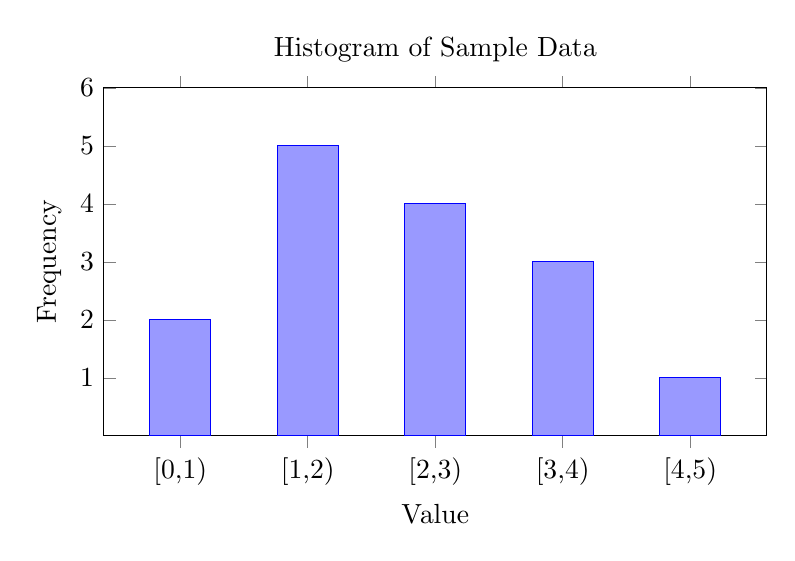
\begin{tikzpicture}
		\pgfplotsset{compat=1.18}
		\begin{axis}[
		    ybar,
		    ymin=0,
		    ymax=6,
		    bar width=22pt,
		    width=10cm,
		    height=6cm,
		    xlabel={Value},
		    ylabel={Frequency},
		    ytick={1,2,3,4,5,6},
		    xtick={1,2,3,4,5},
		    xticklabels={{[0,1)}, {[1,2)}, {[2,3)}, {[3,4)}, {[4,5)}},
		    enlarge x limits=0.15,
		    title={Histogram of Sample Data}
			]
		\addplot+[fill=blue!40] coordinates {(1,2) (2,5) (3,4) (4,3) (5,1)};
		\end{axis}
		\end{tikzpicture}
		\caption{A histogram representing the frequency of data points falling within discrete value ranges (i.e., bins). 
		Each bar height shows the count of samples in the corresponding interval.}
		\label{fig:histogram_dict}
		\end{figure}
		See also: dataset, data point, sample.},
	first={histogram},
	text={histogram}  
}

\newglossaryentry{bootstrap}
{name={bootstrap},
	description={For the analysis of ML methods, it is often useful to interpret 
		a given set of data points $\mathcal{D} = \big\{ {\bf z}^{(1)}, \,\ldots, \,{\bf z}^{(m)}\big\}$ 
		as realizations of iid RVs drawn from a common probability distribution $p({\bf z})$. 
		In practice, the probability distribution $p({\bf z})$ is unknown and must be estimated from $\mathcal{D}$. 
		The bootstrap approach uses the histogram of $\mathcal{D}$ as an estimator for $p({\bf z})$. 
				\\
		See also: iid, RV, probability distribution, histogram.},
	first={bootstrap},
	text={bootstrap}  
}

\newglossaryentry{featurespace}
{name={feature space},
	description={The feature space of a given ML application 
		or method is constituted by all potential values that the feature vector of a data point can take on. 
		\begin{figure}[H]
			\centering
			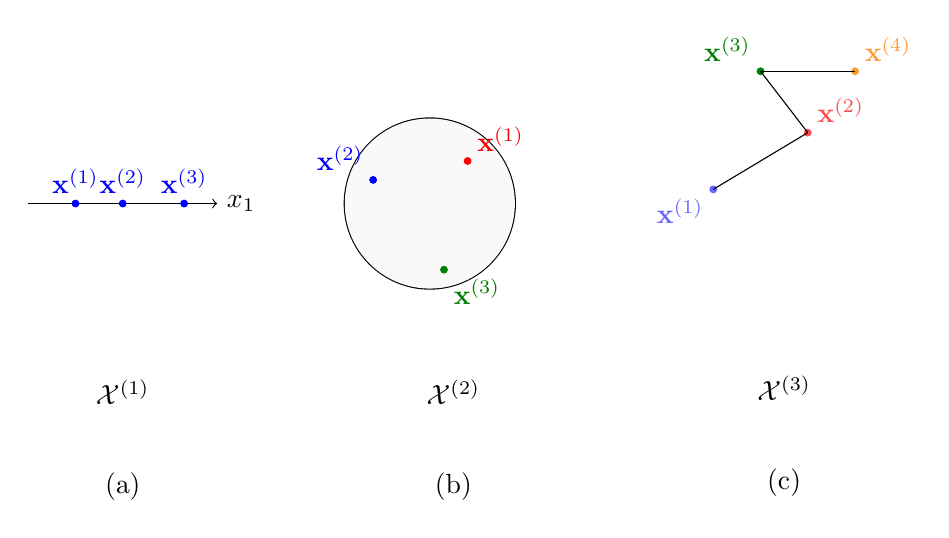
\begin{tikzpicture}[scale=0.6]
			
			\begin{scope}[xshift=0cm]
  				
 	 			\draw[->] (-0.5, 0) -- (3.5, 0) node[right] {$x_1$};
  				
  				\foreach \x/\lbl in {0.5/${\bf x}^{(1)}$, 1.5/${\bf x}^{(2)}$, 2.8/${\bf x}^{(3)}$}
    				\filldraw[blue] (\x,0) circle (2pt) node[above] {\lbl};
  				
  				\node at (1.5, -4.0)  {$\mathcal{X}^{(1)}$};
				\node at (1.5, -6) {(a)};
			\end{scope}
			
			\begin{scope}[xshift=8cm]
  				
  				\draw[thick] (0,0) circle (1.8);
  				\fill[gray!5] (0,0) circle (1.8);
  				
  				\filldraw[red] (0.8, 0.9) circle (2pt) node[anchor=south west] {${\bf x}^{(1)}$};
  				\filldraw[blue] (-1.2, 0.5) circle (2pt) node[anchor=south east] {${\bf x}^{(2)}$};
  				\filldraw[green!50!black] (0.3, -1.4) circle (2pt) node[anchor=north west] {${\bf x}^{(3)}$};
  				
  				\node at (0.5, -4) {$\mathcal{X}^{(2)}$};
				\node at (0.5, -6) {(b)};
			\end{scope}
			
			\begin{scope}[xshift=14cm, yshift=0.3cm]
  				
 	 			\filldraw[blue!60] (0,0) circle (2pt) node[anchor=north east] {${\bf x}^{(1)}$};
 	 			\filldraw[red!70] (2,1.2) circle (2pt) node[anchor=south west] {${\bf x}^{(2)}$};
  				\filldraw[green!50!black] (1,2.5) circle (2pt) node[anchor=south east] {${\bf x}^{(3)}$};
  				\filldraw[orange!80] (3,2.5) circle (2pt) node[anchor=south west] {${\bf x}^{(4)}$};
  				
  				\draw[-] (0,0) -- (2,1.2);
  				\draw[-] (2,1.2) -- (1,2.5);
  				\draw[-] (1,2.5) -- (3,2.5);
  				
  				\node at (1.5, -4.2) {$\mathcal{X}^{(3)}$};
				\node at (1.5, -6.2) {(c)};
			\end{scope}
			\end{tikzpicture}
		\caption{Three different feature spaces. (a) A linear space $\mathcal{X}^{(1)} = \mathbb{R}$. (b) A 
		bounded convex set $\mathcal{X}^{(2)} \subseteq \mathbb{R}^{2}$. (c) A discrete space 
		$\mathcal{X}^{(3)}$ whose elements are nodes of an undirected graph.}
		\end{figure}
		For data points described by a fixed number $d$ of numerical features, 
		a common choice for the feature space is the Euclidean space $\mathbb{R}^{d}$. 
		However, the mere presence of $d$ numeric features does not imply that $\mathbb{R}^{d}$ 
		is the most appropriate representation of the feature space. Indeed, the numerical features  
		might be assigned to data points in a largely arbitrary or random manner, resulting 
		in data points that are randomly scattered throughout $\mathbb{R}^{d}$ 
		without any meaningful geometric structure. Feature learning methods try to learn a 
		transformation of the original (potentially non-numeric) features to ensure a 
		more meaningful arrangement of data points in $\mathbb{R}^{d}$. 
				\\
		See also: feature vector, Euclidean space.},
	first={feature space},
	text={feature space}  
}


\newglossaryentry{missingdata}
{name={missing data},
	description={Consider a dataset constituted by data points collected via 
		some physical device. Due to imperfections and failures, some of the feature 
		or label values of data points might be corrupted or simply missing. 
		Data imputation aims to estimate these missing values \cite{Abayomi2008DiagnosticsFM}. 
		We can interpret data imputation as an ML problem where the label of a data point is 
		the value of the corrupted feature.
				\\
		See also: feature, label. },
	first={missing data},
	text={missing data}  
}


\newglossaryentry{psd}
{name={positive semi-definite (psd)},
	description={A (real-valued) symmetric matrix $\mathbf{Q} = \mathbf{Q}\,^{T} \in \mathbb{R}^{d \times d}$ 
	 	is referred to as psd if ${\bf x}\,^{T} \mathbf{Q} {\bf x} \geq 0$ for every vector ${\bf x} \in \mathbb{R}^{d}$. 
	 	The property of being psd can be extended from matrices to (real-valued) 
	 	symmetric kernel maps $K: \mathcal{X} \times \mathcal{X} \rightarrow \mathbb{R}$ 
	 	(with $K({\bf x},{\bf x}') = K({\bf x}',{\bf x})$)
	 	as follows: For any finite set of feature vectors ${\bf x}^{(1)}, \,\ldots, \,{\bf x}^{(m)}$, 
	 	the resulting matrix $\mathbf{Q} \in \mathbb{R}^{m \times m}$ with 
		entries $Q_{r,r'} = K\big({\bf x}^{(r)},{\bf x}^{(r')}\big)$ 
		is psd \cite{LearningKernelsBook}.
			\\
		See also: matrix, vector, kernel, map, feature vector.},
	first={positive semi-definite (psd)},
	text={psd}  
}

\newglossaryentry{feature}
{name={feature}, plural={features},
	description={A feature of a data point is one of its properties that can be 
		measured or computed easily without the need for human supervision. For example, if a data point 
		is a digital image (e.g., stored as a \texttt{.jpeg} file), then we could use the red-green-blue intensities 
		of its pixels as features. Domain-specific synonyms for the term feature are "covariate," "explanatory variable," 
		"independent variable," "input (variable)," "predictor (variable)," or "regressor" \cite{Gujarati2021}, \cite{Dodge2003}, \cite{Everitt2022}. 
				\\
		See also: data point.}, 
	first={feature},
	text={feature}  
}

\newglossaryentry{featurevec}
{name={feature vector}, plural={feature vectors},
	description={Feature vector refers to a vector ${\bf x} = \big(x_{1}, \,\ldots, \,x_{d}\big)\,^{T}$ 
		whose entries are individual features $x_{1}, \,\ldots, \,x_{d}$. Many ML methods 
		use feature vectors that belong to some finite-dimensional Euclidean space $\mathbb{R}^{d}$. 
		For some ML methods, however, it can be more convenient to work with feature 
		vectors that belong to an infinite-dimensional vector space (e.g., see kernel method). 
			\\
		See also: feature, vector, ML, Euclidean space, vector space.}, 
	first={feature vector},
	text={feature vector}  
}


\newglossaryentry{label}
{name={label}, plural={labels},
	description={A higher level fact or quantity of interest associated with a data point. 
		For example, if the data point is an image, the label could indicate whether the 
		image contains a cat or not. Synonyms for label, commonly used in specific domains, 
		include "response variable," "output variable," and "target" \cite{Gujarati2021}, \cite{Dodge2003}, \cite{Everitt2022}.
				\\
		See also: data point.},
	first={label},
	text={label}  
}


\newglossaryentry{data}
{name={data},
	 description={Data refer to objects that carry information. These 
	 	objects can be either concrete physical objects (such as persons or animals) 
	 	or abstract concepts (such as numbers). We often use representations (or 
	 	approximations) of the original data that are more convenient for data processing. 
	 	These approximations use different mathematical structures such as relations 
		that are used in relational databases \cite{codd1970relational}, \cite{silberschatz2019database}.
				\\
		See also: model, dataset, data point.}, 
	text={data}
}

\newglossaryentry{dataset}
{name={dataset}, plural={datasets},
	description={A dataset refers to a collection of data points. These 
		data points carry information about some quantity of interest (or label) within 
		an ML application. ML methods use datasets for model training (e.g., via ERM)
		and model validation. Note that our notion of a dataset is very flexible, as 
		it allows for very different types of data points. Indeed, data points can be concrete 
		physical objects (such as humans or animals) or abstract objects (such as numbers). 
		As a case in point, Fig. \ref{fig_cows_dataset_dict} depicts a dataset that consists of cows as 
		data points. 
		\begin{figure}[H]
			\begin{center}
			\label{fig:cowsintheswissalps_dict}
			\includegraphics[width=0.5\textwidth]{assets/CowsAustria.jpg}
		  	\end{center}
			\caption{\label{fig_cows_dataset_dict}A cow herd somewhere in the Alps.}
	 	\end{figure}
       		Quite often, an ML engineer does not have direct access to a dataset. Indeed, accessing the 
       		dataset in Fig. \ref{fig_cows_dataset_dict} would require us to visit the cow herd in the Alps. Instead, 
       		we need to use an approximation (or representation) of the dataset that is more convenient 
       		to work with. Different mathematical models have been developed for the representation (or approximation) 
       		of datasets \cite{silberschatz2019database}, \cite{abiteboul1995foundations}, \cite{hoberman2009data}, \cite{ramakrishnan2002database}. 
       		One of the most widely adopted data model is the relational model, which organizes data 
       		as a table (or relation) \cite{codd1970relational}, \cite{silberschatz2019database}.
		A table consists of rows and columns, where each row of the table represents a single data point, and 
		each column of the table corresponds to a specific attribute of the data point. 
		ML methods can use attributes as features and labels of the data point.\\
		For example, Table~\ref{tab:cowdata_dict} shows a representation of the dataset in Fig. \ref{fig_cows_dataset_dict}. 
		In the relational model, the order of rows is irrelevant, and each attribute (i.e., column) must be 
		precisely defined with a domain, which specifies the set of possible values. In ML applications, 
		these attribute domains become the feature space and the label space.
		\begin{table}[H]
			\refstepcounter{table}
			\caption*{
				\centering 
				\scshape TABLE \thetable \\[0.5ex]
				\scshape A Relation (or Table) That Represents the Dataset in Fig. \ref{fig_cows_dataset_dict} 
			}
			\label{tab:cowdata_dict} 
			\centering
			\begin{tabular}{lcccc}
				\hline
				\textbf{Name} & \textbf{Weight} & \textbf{Age} & \textbf{Height} & \textbf{Stomach temperature} \\
				\hline
				Zenzi & 100 & 4 & 100 & 25 \\
				Berta & 140 & 3 & 130 & 23 \\
				Resi  & 120 & 4 & 120 & 31 \\
				\hline
			\end{tabular}
		\end{table}
 		While the relational model is useful for the study of many ML applications, it may be 
 		insufficient regarding the requirements for trustworthy AI. Modern 
 		approaches like datasheets for datasets provide more comprehensive 
 		documentation, including details about the data collection process, intended 
 		use, and other contextual information \cite{DatasheetData2021}.
 		\\
		See also: data point, data, feature, feature space, label space, trustworthy AI.},
	first={dataset},
	text={dataset}  
}

\newglossaryentry{predictor}
{name={predictor},
	description={A predictor is a real-valued hypothesis map. 
		Given a data point with features ${\bf x}$, the value 
		$h({\bf x}) \in \mathbb{R}$ is used as a prediction for the true 
		numeric label $y \in \mathbb{R}$ of the data point.
				\\
		See also: hypothesis, map, data point, feature, prediction, label. },
	first={predictor},
	text={predictor}  
}

\newglossaryentry{labeled datapoint}
{name={labeled data point}, plural={labeled data points},
 	description={A data point whose label is known or has been determined 
 		by some means that might require human labor.
			\\
		See also: data point, label.},
 	first={labeled data point},
 	text={labeled data point}  
}

\newglossaryentry{rv}
{name={random variable (RV)}, plural={RVs},
 	description={An RV is a function that maps the 
		outcomes of a random experiment to a value space \cite{BillingsleyProbMeasure}, \cite{GrayProbBook}. 
 		Mathematically, a RV is a function $x: \Omega \rightarrow \mathcal{X}$ that is defined on the 
		sample space $\Omega$ of a probability space.
 		Different types of RVs include  
 		\begin{itemize} 
 			\item {binary RVs}, which map each outcome to an element of a binary set (e.g., $\{-1,1\}$ or $\{\text{cat}, \text{no cat}\}$); 
 			\item {real-valued RVs}, which take on values in the real numbers $\mathbb{R}$;  
 			\item {vector-valued RVs}, which map outcomes to the Euclidean space $\mathbb{R}^{d}$.  
 		\end{itemize} 
 		Probability theory uses the concept of measurable spaces to rigorously define 
 		and study the properties of collections of RVs \cite{BillingsleyProbMeasure}.
			\\
		See also: function, random experiment, sample space, probability space, vector, Euclidean space, probability, measurable.}, 
	first={random variable (RV)},
	text={RV}  
}
 
 \newglossaryentry{probspace}
 {name={probability space}, 
 	description={A probability space is a mathematical 
 		structure that allows us to reason about a random experiment, e.g., the observation 
		of a physical phenomenon. 
 	   	Formally, a probability space $\mathcal{P}$ is a triplet $(\Omega, \mathcal{F}, \mathbb{P}({\cdot}))$ where
 		\begin{itemize} 
 			\item  $\Omega$ is a sample space containing all possible outcomes of a random experiment;
 			\item  $\mathcal{F}$ is a $\sigma$-algebra, i.e., a collection of subsets of $\Omega$ (called events) that satisfies 
 			certain closure properties under set operations;
 			\item $\mathbb{P}({\cdot})$ is a probability distribution, i.e., a function that assigns a probability $P(\mathcal{A}) \in [0,1]$ 
 			to each event $\mathcal{A} \in \mathcal{F}$. This function must satisfy $\mathbb{P}({\Omega}) = 1$ and 
			$\mathbb{P}({\bigcup_{i=1}^{\infty} \mathcal{A}_i}) = \sum_{i=1}^{\infty} \mathbb{P}({\mathcal{A}_i})$ for any 
 			countable sequence of pairwise disjoint events $\mathcal{A}_1, \,\mathcal{A}_2, \,\ldots$ in $\mathcal{F}$.
 		\end{itemize}
 		Probability spaces provide the foundation of probabilistic models that can be 
		used to study the behavior of ML methods \cite{BillingsleyProbMeasure}, \cite{GrayProbBook}, \cite{ross2013first}.
				\\
		See also: probability, random experiment, sample space, event, probability distribution, function, probabilistic model, ML.},  
 	first={probability space}, 
 	text={probability space}
 }
 
 
 \newglossaryentry{samplespace}
  {name={sample space}, 
  	description={A sample space is the set of all possible 
		outcomes of a random experiment \cite{BillingsleyProbMeasure}, 
		\cite{BertsekasProb}, \cite{papoulis}, \cite{AshProbMeasure}. 
		\\
 		See also: probability space.},  
  	first={sample space}, 
 	firstplural={sample spaces},
 	plural={sample spaces},
  	text={sample space}
  }
 
	
\newglossaryentry{realization}
{name={realization}, plural={realizations},
	description={Consider an RV ${\bf x}$ that maps each outcome 
		$\omega \in \mathcal{P}$ of a probability space $\mathcal{P}$ to an element $a$ of a measurable space 
		$\mathcal{N}$ \cite{RudinBookPrinciplesMatheAnalysis}, \cite{BillingsleyProbMeasure}, \cite{HalmosMeasure}. 
		A realization of ${\bf x}$ is any element ${\bf a} \in \mathcal{N}$ such that there is 
		an element $\omega' \in \mathcal{P}$ with ${\bf x}(\omega') = {\bf a}$.
			\\
		See also: RV, probability space, measurable.}, 
	first={realization},
	text={realization}  
}

\newglossaryentry{trainset}
{name={training set}, plural={training sets},
	description={A training set is a dataset $\mathcal{D}$ that consists of some data points used in ERM 
		to learn a hypothesis $\hat{h}$. The average loss of $\hat{h}$ on the 
		training set is referred to as the training error. The comparison of the training error with the 
		validation error of $\hat{h}$ allows us to diagnose the ML method and informs how to improve 
		the validation error (e.g., using a different hypothesis space or collecting more data points) \cite[Sec. 6.6]{MLBasics}.
			\\
		See also: dataset, data point, ERM, hypothesis, loss, training error, validation error, ML, hypothesis space.},
	first={training set},
	text={training set}  
}

\newglossaryentry{netmodel}
{name={networked model},
 	description={A networked model over an FL network $\mathcal{G} = \left( \mathcal{V},\mathcal{E} \right)$ assigns 
   		a local model (i.e., a hypothesis space) to each node $i \in \mathcal{V}$ of the FL network $\mathcal{G}$.
   		\\
		See also: model, FL network, local model, hypothesis space.}, 
   first={networked model},
   text={networked model}  
}

\newglossaryentry{batch}
{name={batch},
	description={In the context of SGD, a batch refers to a randomly 
		chosen subset of the overall training set. We use the data points in this subset 
		to estimate the gradient of training error and, in turn, to update the model parameters.
			\\
		See also: SGD, training set, data point, gradient, training error, model parameters.}, 
 	first={batch},
 	firstplural={batches}, 
 	plural={batches}, 
 	text={batch}  
}

\newglossaryentry{netdata}
{name={networked data},
	description={Networked data consist of local datasets 
		that are related by some notion of pairwise similarity. We can represent networked 
		data using a graph whose nodes carry local datasets and edges encode 
		pairwise similarities. An example of networked data can be found in FL applications 
		where local datasets are generated by spatially distributed devices.
			\\
		See also: data, local dataset, graph, FL, device.}, 
	first={networked data},
	text={networked data}  
}

\newglossaryentry{trainerr}
{name={training error},
	description={The average loss of a hypothesis when 
		predicting the labels of the data points in a training set. 
		We sometimes refer by training error also to minimal average loss 
		that is achieved by a solution of ERM.
				\\
		See also: loss, hypothesis, label, data point, training set, ERM.},
	first={training error},
	text={training error}  
}

\newglossaryentry{datapoint}
{name={data point}, plural={data points},
	description={A data point is any object that conveys information~\cite{coverthomas}. 
		Examples include students, radio signals, trees, images, RVs, real numbers, 
 		or proteins. We describe data points of the same type by two categories 
		of properties. The first category includes features that are measurable or computable properties of a 
		data point. These attributes can be automatically extracted or computed using sensors, computers, or other
		data collection systems. For a data point that represents a patient, one feature could be the body weight.
    		The second category includes labels that are higher level facts (or quantities of interest) 
		associated with the data point. Determining the labels of a data point 
		usually requires human expertise or domain knowledge. For a data point that represents a patient, 
		a cancer diagnosis provided by a physician would serve as the label. 
		Fig.\ \ref{fig:datapoint_cowherd_dict} depicts an image as an example of a data 
		point along with its features and labels. Importantly, what constitutes 
		a feature or a label is not inherent to the data point itself—it is a design 
		choice that depends on the specific ML applicaton.
		\begin{figure}[H]
    		\centering
    			
    			\begin{minipage}[t]{0.95\textwidth}
        			\centering
        			\includegraphics[width=\textwidth]{assets/CowsAustria.jpg}
        			\caption*{A single data point.}
        			\vspace{5mm}
    			\end{minipage}
    			
    			\begin{minipage}[t]{0.95\textwidth}
        			Features:
        			\begin{itemize}
            			\item $x_{1}, \,\ldots, \,x_{d_{1}}$: Color intensities of all image pixels.
            			\item $x_{d_{1}+1}$: Time-stamp of the image capture.
            			\item $x_{d_{1}+2}$: Spatial location of the image capture.
			\end{itemize}
			Labels:
            		\begin{itemize}
               	 		\item $y_{1}$: Number of cows depicted. 
                			\item $y_{2}$: Number of wolves depicted. 
                			\item $y_{3}$: Condition of the pasture (e.g., healthy, overgrazed).
            		\end{itemize}
    			\end{minipage}
    			\caption{Illustration of a data point consisting of an image. We can use 
			different properties of the image as features and higher level facts
			about the image as labels.\label{fig:datapoint_cowherd_dict}}
		\end{figure}
 		The distinction between features and labels is not always clear-cut. 
 		A property that is considered a label in one setting (e.g., a cancer diagnosis) 
 		may be treated as a feature in another setting—particularly if reliable automation (e.g., 
 		via image analysis) allows it to be computed without human intervention.
   		ML broadly aims to predict the label of a data point based on its features. 
				\\
		See also: data, feature, label, dataset.}, 
	first={data point},
	text={data point}  
}


\newglossaryentry{valerr}
{name={validation error}, plural={validation errors},
 	description={Consider a hypothesis $\hat{h}$ that is 
 		obtained by some ML method, e.g., using ERM on a training set. The average loss 
 		of $\hat{h}$ on a validation set, which is different from the training set, is referred 
 		to as the validation error.
			\\
		See also: hypothesis, ML, ERM, training set, loss, validation set, validation.},
	first={validation error},
	text={validation error}  
}

\newglossaryentry{validation} 
{name={validation},
	description={Consider a hypothesis $\hat{h}$ that has been 
		learned via some ML method, e.g., by solving ERM on a training set $\mathcal{D}$. 
		Validation refers to the practice of evaluating the loss incurred by the 
		hypothesis $\hat{h}$ on a set of 
		data points that are not contained in the training set $\mathcal{D}$.
				\\
		See also: hypothesis, ML, ERM, training set, loss, data point. },
	first={validation},
	text={validation}  
}

\newglossaryentry{quadfunc}
{name={quadratic function},
	description={A function $f: \mathbb{R}^{d} \rightarrow \mathbb{R}$ of the form 
		$$f({\bf w}) =  {\bf w}\,^{T} \mathbf{Q} \mathbf{w} + \mathbf{q}\,^{T} {\bf w}+a$$ with 
		some matrix $\mathbf{Q} \in \mathbb{R}^{d \times d}$, vector ${\bf q} \in \mathbb{R}^{d}$, 
		and scalar $a \in \mathbb{R}$.
		\\
		See also: function, matrix, vector. },
	first={quadratic function},
	text={quadratic function}  
}

\newglossaryentry{valset}
{name={validation set},
 	description={A set of data points used to estimate 
  		the risk of a hypothesis $\hat{h}$ that has been learned by some 
  		ML method (e.g., solving ERM). The average loss of $\hat{h}$ 
  		on the validation set is referred to as the validation error and can be used to diagnose an 
  		ML method (see \cite[Sec. 6.6]{MLBasics}). The comparison between training error 
  		and validation error can inform directions for the improvement of the ML method (such as 
  		using a different hypothesis space).
			\\
		See also: data point, risk, hypothesis, ML, ERM, loss, validation, validation error, training error, hypothesis space.},
	first={validation set},
	text={validation set}  
}

\newglossaryentry{testset}
{name={test set},
	description={A set of data points that have  
		been used neither to train a model (e.g., via ERM) nor in a validation set 
		to choose between different models.
				\\
		See also: data point, model, ERM, validation set.},
	first={test set},
	text={test set}  
}


\newglossaryentry{modelsel}
{name={model selection},
	description={In ML, model selection refers to the 
		process of choosing between different candidate models. In its most 
		basic form, model selection amounts to: 1) training each candidate model; 
		2) computing the validation error for each trained model; and 3) choosing the model 
		with the smallest validation error \cite[Ch. 6]{MLBasics}. 
				\\
		See also: ML, model, validation error.},
	first={model selection},
	text={model selection}  
}


\newglossaryentry{linclass}
{name={linear classifier}, 
	description={Consider data points characterized by numeric features ${\bf x} \in \mathbb{R}^{d}$ 
	    	and a label $y \in \mathcal{Y}$ from some finite label space $\mathcal{Y}$. 
		A linear classifier is characterized by having decision regions that are 
		separated by hyperplanes in $\mathbb{R}^{d}$ \cite[Ch. 2]{MLBasics}.
				\\
		See also: data point, feature, label, label space, classifier, decision region.},
	first={linear classifier},
	text={linear classifier} 
}


\newglossaryentry{erm}
{name={empirical risk minimization (ERM)}, 
	description={ERM is the optimization problem of finding 
		a hypothesis (from a model) with the minimum average loss (or empirical risk) on a given dataset 
		$\mathcal{D}$ (i.e., the training set). Many ML methods are obtained from 
		empirical risk via specific design choices for the dataset, model, and loss \cite[Ch. 3]{MLBasics}.
				\\
		See also: optimization problem, hypothesis, model, minimum, loss, empirical risk, dataset, training set, ML.},
	first={empirical risk minimization (ERM)},
	text={ERM} 
}


\newglossaryentry{multilabelclass}
{name={multi-label classification}, 
	description={Multi-label 
		classification problems and methods use data points 
		that are characterized by several labels. As an example, consider a data point 
		representing a picture with two labels. One label indicates the presence of a human 
		in this picture and another label indicates the presence of a car.
				\\
		See also: label, classification, data point.},
	    first={multi-label classification},
	    text={multi-label classification} 
}


\newglossaryentry{ssl}
{name={semi-supervised learning (SSL)}, 
	description={SSL methods use unlabeled data points
		to support the learning of a hypothesis from labeled data points \cite{SemiSupervisedBook}. 
		This approach is particularly useful for ML applications that offer a large amount of 
		unlabeled data points, but only a limited number of labeled data points.
			\\
		See also: data point, hypothesis, labeled data point, ML.}, 
	first={semi-supervised learning (SSL)},
	text={SSL} 
}
	
	
\newglossaryentry{objfunc}
{name={objective function}, plural={objective functions}, 
	description={An objective function is a map that assigns a numeric 
		objective value $f({\bf w})$ to each choice ${\bf w}$ of some variable that we want to 
		optimize (see Fig. \ref{fig_obj_func_dict}). In the context of ML, the optimization variable could 
		be the model parameters of a hypothesis $h^{({\bf w})}$. 
		Common objective functions include the risk (i.e., expected loss) or the empirical risk 
		(i.e., average loss over a training set). ML methods apply optimization 
		techniques, such as gradient-based methods, to find the choice ${\bf w}$ with the 
		optimal value (e.g., the minimum or the maximum) of the objective function.
		\\
		\begin{figure}[H]
			\begin{center}
			\begin{tikzpicture}[scale=1.0]
				
				\draw[->] (-0.5,0) -- (4.5,0) node[right] {${\bf w}$};
				\draw[->] (0,-0.5) -- (0,3.5);
				
				\draw[thick,domain=0.3:4,smooth,variable=\x] 
				plot ({\x}, {0.5*(\x-2)^2 + 0.5});
				
				\node at (3.5,2.8) {$f({\bf w})$};
			\end{tikzpicture} 
			\end{center}
		\caption{An objective function maps each possible value ${\bf w}$ of an optimization variable, such 
		as the model parameters of an ML model, to a value that measures the usefulness 
	   	of ${\bf w}$.\label{fig_obj_func_dict}}
		\end{figure} 
		See also: function, map, ML, model parameters, hypothesis, risk, loss, empirical risk, training set, gradient-based methods, minimum, maximum, model, loss function.},
	first={objective function},
	text={objective function} 
}
	
\newglossaryentry{regularizer}
{name={regularizer}, 
	description={A regularizer 
		assigns each hypothesis $h$ from a hypothesis space $\mathcal{H}$ a quantitative 
		measure $\mathcal{R}\big\{ h \big\}$ conveying to what extent its prediction errors might differ 
		on data points on and outside a training set. Ridge regression 
		uses the regularizer $\mathcal{R}\big\{ h \big\} := \left\Vert  {{\bf w}} \right\Vert_{2}^{2}$ for linear hypothesis 
		maps $h^{({\bf w})}({\bf x}) := {\bf w}\,^{T} {\bf x}$ \cite[Ch. 3]{MLBasics}. 
		Lasso uses the regularizer $\mathcal{R}\big\{ h \big\} := \left\Vert  {{\bf w}} \right\Vert_{1}$ 
		for linear hypothesis maps $h^{({\bf w})}({\bf x}) := {\bf w}\,^{T} {\bf x}$ \cite[Ch. 3]{MLBasics}.
				\\
		See also: hypothesis, hypothesis space, prediction, training set, data point, ridge regression, map, Lasso. },
	first={regularizer},
	text={regularizer} 
}


\newglossaryentry{regularization}
{name={regularization}, 
	description={A key challenge of modern ML applications is that they often 
		use large models, which have an effective dimension in the order of billions. 
		Training a high-dimensional model using basic ERM-based methods
		is prone to overfitting, i.e., the learned hypothesis performs well on the training set 
		but poorly outside the training set. Regularization refers to modifications of a given instance 
		of ERM in order to avoid overfitting, i.e., to ensure that the learned hypothesis does 
		not perform much worse outside the training set. There are three routes for implementing 
		regularization: 
		\begin{enumerate}[label=\arabic*)]
			\item {Model pruning:} We prune the original model $\mathcal{H}$ to obtain a 
			smaller model $\mathcal{H}'$. For a parametric model, the pruning can be 
			implemented via constraints on the model parameters (such as $w_{1} \in [0.4,0.6]$ for 
			the weight of feature $x_{1}$ in linear regression).
			\item {Loss penalization:} We modify the objective function of ERM by adding a 
			penalty term to the training error. The penalty term estimates how much larger the expected loss (or risk) 
			is compared to the average loss on the training set. 
			\item {Data augmentation:} We can enlarge the training set $\mathcal{D}$ by adding 
			perturbed copies of the original data points in $\mathcal{D}$. One example for such 
			a perturbation is to add the realization of an RV to the feature vector 
			of a data point. 
		\end{enumerate} 
		Fig. \ref{fig_equiv_dataaug_penal_dict} illustrates the above three routes to regularization. 
		These routes are closely related and sometimes fully equivalent. Data augmentation using Gaussian RVs 
		to perturb the feature vectors in the training set of linear regression 
		has the same effect as adding the penalty 
		$\lambda \left\Vert  {{\bf w}} \right\Vert_{2}^2$ to the training error (which is nothing but ridge regression). 
        		The decision on which route to use for regularization can be based on the 
        		available computational infrastructure. For example, it might be much easier to 
        		implement data augmentation than model pruning. 
		\begin{figure}[H]
			\begin{center} 
				\begin{tikzpicture}[scale = 1]
					
					\draw[->, very thick] (0,0.5) -- (7.7,0.5) node[right] {feature $x$};       
					\draw[->, very thick] (0.5,0) -- (0.5,4.2) node[above] {label $y$};   
					\draw[color=black, thick, dashed, domain = -1: 6.2, variable = \x]  plot ({\x},{\x*0.4 + 2.0}) ;     
					\draw[color=black, thick, dashed, domain = -1: 6.2, variable = \x]  plot ({\x},{\x*0.6 + 2.0}) ;     
					
	          			
					\draw[blue, thick] (5, 4.5) ellipse [x radius=0.2cm, y radius=1cm];
					\node at (5, 5.8) [text=black, font=\small] {$\{ h: h(x)\!=\!w_{1}x\!+\!w_{0}; w_{1} \in [0.4,0.6]\}$};
					\node at (6.7,4.5) {$h(x)$};    
					\coordinate (l1)   at (1.2, 2.48);
					\coordinate (l2) at (1.4, 2.56);
					\coordinate (l3)   at (1.7,  2.68);
					\coordinate (l4)   at (2.2, 2.2*0.4+2.0);
					\coordinate (l5) at (2.4, 2.4*0.4+2.0);
					\coordinate (l6)   at (2.7,  2.7*0.4+2.0);
					\coordinate (l7)   at (3.9,  3.9*0.4+2.0);
					\coordinate (l8) at (4.2, 4.2*0.4+2.0);
					\coordinate (l9)   at (4.5,  4.5*0.4+2.0);
					\coordinate (n1)   at (1.2, 1.8);
					\coordinate (n2) at (1.4, 1.8);
					\coordinate (n3)   at (1.7,  1.8);
					\coordinate (n4)   at (2.2, 3.8);
					\coordinate (n5) at (2.4, 3.8);
					\coordinate (n6)   at (2.7,  3.8);
					
					\coordinate (n7)   at (3.9, 2.6);
					\coordinate (n8) at (4.2, 2.6);
					\coordinate (n9)   at (4.5,  2.6);
					\node at (n1)  [circle,draw,fill=red,minimum size=6pt,scale=0.6, name=c1] {};
					\node at (n2)  [circle,draw,fill=blue,minimum size=6pt, scale=0.6, name=c2] {};
					\node at (n3)  [circle,draw,fill=red,minimum size=6pt,scale=0.6,  name=c3] {};
					\node at (n4)  [circle,draw,fill=red,minimum size=12pt, scale=0.6, name=c4] {};  
					\node at (n5)  [circle,draw,fill=blue,minimum size=12pt,scale=0.6,  name=c5] {};
					\node at (n6)  [circle,draw,fill=red,minimum size=12pt, scale=0.6, name=c6] {};  
					\node at (n7)  [circle,draw,fill=red,minimum size=12pt,scale=0.6,  name=c7] {};
					\node at (n8)  [circle,draw,fill=blue,minimum size=12pt, scale=0.6, name=c8] {};
					\node at (n9)  [circle,draw,fill=red,minimum size=12pt, scale=0.6, name=c9] {};
					\draw [<->] ($ (n7) + (0,-0.3) $)  --  ($ (n9) + (0,-0.3) $) node [pos=0.4, below] {$\sqrt{\alpha}$}; ; 
					\draw[<->, color=red, thick] (l1) -- (c1);  
					\draw[<->, color=blue, thick] (l2) -- (c2);  
					\draw[<->, color=red, thick] (l3) -- (c3);  
					\draw[<->, color=red, thick] (l4) -- (c4);  
					\draw[<->, color=blue, thick] (l5) -- (c5);  
					\draw[<->, color=red, thick] (l6) -- (c6);  
					\draw[<->, color=red, thick] (l7) -- (c7);  
					\draw[<->, color=blue, thick] (l8) -- (c8);  
					\draw[<->, color=red, thick] (l9) -- (c9);  
					\draw[fill=blue] (6.2, 3.7)  circle (0.1cm) node [black,xshift=2.3cm] {original training set $\mathcal{D}$};
					\draw[fill=red] (6.2, 3.2)  circle (0.1cm) node [black,xshift=1.3cm] {augmented};
					\node at (4.6,1.2)  [minimum size=12pt, font=\fontsize{12}{0}\selectfont, text=blue] {$\frac{1}{m} \sum\limits_{r=1}^m L\left(\left( {\bf x}^{(r)}, y^{(r)} \right),h \right)$};
					\node at (7.8,1.2)  [minimum size=12pt, font=\fontsize{12}{0}\selectfont, text=red] {$+\alpha \mathcal{R}\big\{ h \big\}$};
				\end{tikzpicture}
				\caption{Three approaches to regularization: 1) data augmentation; 2) loss penalization; and 3) model 
				pruning (via constraints on model parameters). \label{fig_equiv_dataaug_penal_dict} }
			\end{center}
		\end{figure} 
		See also: overfitting, data augmentation, validation, model selection.},
	first={regularization},
	text={regularization} 
}
	

\newglossaryentry{rerm}
{name={regularized empirical risk minimization (RERM)}, 
	description={Basic ERM learns a hypothesis (or trains a model) $h \in \mathcal{H}$ 
		based solely on the empirical risk $\widehat{L}\big(h|\mathcal{D}\big)$ incurred on a training set $\mathcal{D}$. 
		To make ERM less prone to overfitting, we can implement regularization by 
		including a (scaled) regularizer $\mathcal{R}\big\{ h \big\}$ in the learning objective. 
		This leads to RERM such that
		\begin{equation}
			\label{equ_def_rerm_dict}
			\hat{h} \in \aargmin_{h \in \mathcal{H}} \widehat{L}\big(h|\mathcal{D}\big) + \alpha \mathcal{R}\big\{ h \big\}.
		\end{equation}
		The parameter $\alpha \geq 0$ controls the regularization strength. 
		For $\alpha = 0$, we recover standard ERM without regularization. As $\alpha$ increases, the 
		learned hypothesis is increasingly biased toward small values of $\mathcal{R}\big\{ h \big\}$. 
		The component $\alpha \mathcal{R}\big\{ h \big\}$ in the objective function of \eqref{equ_def_rerm_dict} 
		can be intuitively understood as a surrogate for the increased average loss that may 
		occur when predicting labels for data points outside the training set. This intuition  
		can be made precise in various ways. For example, consider a linear model trained using squared error loss 
		and the regularizer $\mathcal{R}\big\{ h \big\} = \left\Vert  {{\bf w}} \right\Vert_{2}^{2}$. 
		In this setting, $\alpha \mathcal{R}\big\{ h \big\}$ corresponds to the expected increase in loss 
		caused by adding Gaussian RVs to the feature vectors in the training set 
		\cite[Ch. 3]{MLBasics}.
		A principled construction for the regularizer $\mathcal{R}\big\{ h \big\}$ 
		arises from approximate upper bounds on the generalization error. The resulting 
		RERM instance is known as SRM \cite[Sec. 7.2]{ShalevShwartz2009}.
				\\
		See also: ERM, hypothesis, model, empirical risk, training set, overfitting, regularization, regularizer, parameter, objective function, loss, label, data point, linear model, squared error loss, Gaussian RV, feature vector, generalization, SRM.}, 
	first={regularized empirical risk minimization (RERM)},
	text={RERM} 
}


\newglossaryentry{generalization}
{name={generalization}, plural={generalizations}, 
	description={Generalization refers to the ability of a model trained on a training set to make accurate 
		predictions on new, unseen data points. This is a central goal of ML and AI, i.e., 
		to learn patterns that extend beyond the training set. Most ML systems 
		use ERM to learn a hypothesis $\hat{h} \in \mathcal{H}$ by minimizing 
		the average loss over a training set of data points ${\bf z}^{(1)}, \,\ldots, \,{\bf z}^{(m)}$, 
		which is denoted $\mathcal{D}^{(\rm train)}$. However, success on the training set does not guarantee success on 
		unseen data—this discrepancy is the challenge of generalization. \\ To study generalization 
		mathematically, we need to formalize the notion of ``unseen'' data. A widely used 
		approach is to assume a probabilistic model for data generation, such as the i.i.d.\ assumption. 
		Here, we interpret data points as independent RVs with an identical 
		probability distribution $p({\bf z})$. This probability distribution, which is assumed fixed but unknown, 
		allows us to define the risk of a trained model $\hat{h}$ as the expected loss
		\[
		\bar{L} \big( \hat{h} \big) =\mathbb{E} _{{\bf z} \sim p({\bf z})} \big\{ L(\hat{h}, {\bf z}) \big\}.
		\]
		The difference between risk $\bar{L} \big( \hat{h} \big) $ and empirical risk $\widehat{L}\big(\hat{h}|\mathcal{D}^{(\rm train)}\big)$ 
		is known as the generalization gap. Tools from probability theory, such as concentration inequalities 
		and uniform convergence, allow us to bound this gap under certain conditions \cite{ShalevMLBook}.\\
		Generalization without probability: Probability theory is one way to study how well a 
		model generalizes beyond the training set, but it is not the only way. Another option is to use 
		simple, deterministic changes to the data points in the training set. The basic idea is that a 
		good model $\hat{h}$ should be robust, i.e., its prediction $\hat{h}({\bf x})$ 
		should not change much if we slightly change the features ${\bf x}$ of a data point ${\bf z}$. 
		\\[1mm] For example, an object detector trained on smartphone photos should still detect the object if a few 
		random pixels are masked \cite{OnePixelAttack}. Similarly, it should deliver the same result if we rotate 
		the object in the image \cite{MallatUnderstandingDeepLearning}.
		  \begin{figure}[H]
		                   	\centering
		                   	\begin{tikzpicture}[scale=0.8]
							   \draw[lightblue, fill=lightblue, opacity=0.5] (3, 2) ellipse (6cm and 2cm);
								\node[black] at (6, 3) {$p({\bf z})$};
		                   		\fill[blue] (1, 3) circle (4pt) node[below, xshift=0pt, yshift=0pt] {${\bf z}^{(1)}$};
		                   		\fill[blue] (5, 1) circle (4pt) node[below] {${\bf z}^{(2)}$};
		                   		\fill[blue] (1.6, 3) circle (3pt);
		                   		\fill[blue] (0.4, 3) circle (3pt);
		                   		\draw[<->, thin] (1, 3) -- (1.6, 3);
		                   		\draw[<->, thin] (1, 3) -- (0.4, 3);
		                   		\fill[blue] (5.6, 1) circle (3pt);
		                   		\fill[blue] (4.4, 1) circle (3pt);
		                   		\draw[<->, thin] (5, 1) -- (5.6, 1);
		                   		\draw[<->, thin] (5, 1) -- (4.4, 1);
		                   		\draw[black, thick, domain=0:6, smooth] plot (\x, {- 1*\x + 5});
		                   		\node[black] at (3, 2.5) [right] {$\hat{h}$};
		                   	\end{tikzpicture}
		                   	\caption{Two data points ${\bf z}^{(1)},{\bf z}^{(2)}$ that are used as a training set 
		                   		to learn a hypothesis $\hat{h}$ via ERM. We can evaluate $\hat{h}$ 
		                   		outside $\mathcal{D}^{(\rm train)}$ either by an i.i.d.\ assumption with some underlying probability distribution $p({\bf z})$ 
		                   		or by perturbing the data points.}
		                   	\label{fig:polynomial_fit_dict}
		      \end{figure}
		See also: ERM, i.i.d.\ assumption, overfitting, validation.},
	first={generalization},
	text={generalization} 
}

\newglossaryentry{gengap}
{name={generalization gap}, 
	description={Generalization gap is the difference between the performance of a 
	     	trained model on the training set $\mathcal{D}^{(\rm train)}$ and its performance on 
		data points outside $\mathcal{D}^{(\rm train)}$. We can make this notion precise by using 
		a probabilistic model that allows us to compute the risk of a trained model 
		as the expected loss. However, the probability distribution underlying this expectation 
		is typically unknown and needs to be somehow estimated. Validation techniques 
		use different constructions of a validation set, which is different from 
		the training set, to estimate the generalization gap.
		\\
		See also: generalization, validation, ERM, loss function.}, 
	first={generalization gap}, 
	text={generalization gap}
} 
	
\newglossaryentry{concentrationinequ}
{name={concentration inequality}, 
	description={An upper bound on the probability that an RV deviates 
		more than a prescribed amount from its expectation \cite{Wain2019}. 
		\\
		See also: probability, RV, expectation.}, 
	first={concentration inequality},
	firstplural={concentration inequalities},
	plural={concentration inequalities},  
	text={concentration inequality}
}


\newglossaryentry{boosting}
{name={boosting}, 
	description={Boosting is an iterative optimization method to learn an accurate 
		hypothesis map (or strong learner) by sequentially combining less accurate 
		hypothesis maps (referred to as weak learners) \cite[Ch. 10]{hastie01statisticallearning}.
		For example, weak learners are shallow decision trees that are combined to 
		obtain a deep decision tree. Boosting can be understood as a generalization 
		of gradient-based methods for ERM using parametric models and smooth loss functions 
		\cite{Friedman2001}. Just as GD iteratively updates model parameters to reduce the empirical risk, 
		boosting iteratively combines (e.g., by summation) hypothesis maps to reduce the empirical risk. 
		A widely used instance of the generic boosting idea is referred to as gradient boosting, which 
		uses gradients of the loss function for combining the weak learners \cite{Friedman2001}. 
		\begin{figure}[H]
			\begin{center}
				\begin{tikzpicture}[scale=1.2]
					
					\draw[->] (-0.5,0) -- (5.5,0) node[right] {$h$};
					\draw[->] (0,-0.5) -- (0,4.5) node[above] {$L\left({\bf z},h \right)$};
					\draw[thick,domain=0.2:5,smooth,variable=\x,blue!60] plot ({\x},{(4 - 1.3*\x + 0.15*\x*\x)});
					\foreach \x/\label in {0.7/$h^{(0)}$, 1.5/$h^{(1)}$, 2.3/$h^{(2)}$, 3.0/$h^{(3)}$} {
						\draw[dashed, gray] (\x, 0) -- (\x, {4 - 1.3*\x + 0.15*\x*\x}); 
						\filldraw[black] (\x, {4 - 1.3*\x + 0.15*\x*\x}) circle (2pt);   
						\node[below] at (\x, -0.1) {\label};                             
					}
				\end{tikzpicture}
			\end{center} 
			\caption{Boosting methods construct a sequence of hypothesis maps $h^{(0)}, \,h^{(1)}, \,\ldots$ 
				            that are increasingly strong learners (i.e., incurring a smaller loss).}
     		\end{figure} 
     		See also: optimization method, hypothesis, map, decision tree, generalization, gradient-based methods, ERM, model, smooth, loss function, GD, model parameters, empirical risk, gradient, loss, gradient step.}, 
	first={boosting}, 
	text={boosting}
} 

	
\newglossaryentry{gtv}
{name={generalized total variation (GTV)}, 
	description={GTV is a 
		measure of the variation of trained local models $h^{(i)}$ 
		(or their model parameters $\mathbf{w}^{(i)}$) assigned to the nodes $i=1, \,\ldots, \,n$ 
		of an undirected weighted graph $\mathcal{G}$ with edges $\mathcal{E}$. Given a measure $d^{(h,h')}$ 
		for the discrepancy between hypothesis maps $h,h'$, the GTV is 
		\begin{equation} 
			\nonumber
			\sum_{\{i,i'\}\in \mathcal{E}} A_{i,i'} 
			d^{(h^{(i)},h^{(i')})}.
		\end{equation}
		Here, $A_{i,i'}>0$ denotes the weight of the undirected edge $\{i,i'\}\in \mathcal{E}$.
				\\
		See also: local model, model parameters, graph, discrepancy, hypothesis, map.},
	first={GTV},
	text={GTV} 
}
	
\newglossaryentry{srm}
{name={structural risk minimization (SRM)}, 
	description={SRM is an
		instance of RERM, with which the model $\mathcal{H}$ can be expressed 
		as a countable union of submodels such that $\mathcal{H} = \bigcup_{n=1}^{\infty} \mathcal{H}^{(n)}$. 
		Each submodel $\mathcal{H}^{(n)}$ permits the derivation of an approximate upper bound 
		on the generalization error incurred when applying ERM to train $\mathcal{H}^{(n)}$. 
		These individual bounds—one for each submodel—are then combined to form a regularizer 
		used in the RERM objective. 
        		These approximate upper bounds (one for each $\mathcal{H}^{(n)}$) are then combined 
		to construct a regularizer for RERM \cite[Sec.\ 7.2]{ShalevMLBook}.
				\\
		See also: RERM, model, generalization, ERM, regularizer, risk.},
	first={structural risk minimization (SRM)},
	text={SRM}
 }

 \newglossaryentry{rlm}
 {name={regularized loss minimization (RLM)},
 	description={See RERM.},
 	text={RLM}
 }
 

\newglossaryentry{datapoisoning}
{name={data poisoning}, 
	description={Data poisoning refers to the intentional manipulation 
  		(or fabrication) of data points to steer the training of an ML model \cite{Liu2021}, \cite{PoisonGAN}. 
  		Data poisoning attacks take various forms, including backdoor and denial-of-service attacks.
  		A backdoor attack implants triggers into training data, so that the trained model 
  		behaves normally on typical feature vectors but misclassifies a feature vector with a trigger pattern.
  		A denial-of-service attack degrades the trained model's overall performance by injecting mislabeled or 
  		adversarial examples to prevent effective learning.
		Data poisoning is particularly concerning in decentralized or distributed ML settings (such as FL), 
		where training data cannot be centrally verified.
				\\
		See also: attack, backdoor, denial-of-service attack, trustworthy AI.},
	first={data poisoning},
	text={data poisoning} 
}
	
	
\newglossaryentry{backdoor}
{name={backdoor}, 
	description={A backdoor attack refers 
		to the intentional manipulation of the training process underlying an ML method. This manipulation 
		can be implemented by perturbing the training set (i.e., through data poisoning) or via the 
		optimization algorithm used by an ERM-based method. The goal of a 
		backdoor attack is to nudge the learned hypothesis $\hat{h}$ 
		toward specific predictions for a certain range of feature values. This range of feature 
		values serves as a key (or trigger) to unlock a backdoor in the sense of 
		delivering anomalous predictions. The key ${\bf x}$ and the corresponding 
		anomalous prediction $\hat{h}({\bf x})$ are only known to the attacker.
				\\
		See also: ML, training set, data poisoning, algorithm, ERM, hypothesis, prediction, feature.},
	first={backdoor},
	text={backdoor} 
}


\newglossaryentry{clustasspt}
{name={clustering assumption}, 
	description={The 
		clustering assumption postulates that data points in a dataset form a (small) number of 
		groups or clusters. Data points in the same cluster are more similar to each 
		other than those outside the cluster \cite{SemiSupervisedBook}. We obtain different 
		clustering methods by using different notions of similarity between data points.
				\\
		See also: clustering, data point, dataset, cluster.},
	first={clustering assumption},
	text={clustering assumption} 
}
	
\newglossaryentry{dosattack}
{name={denial-of-service attack}, plural={denial-of-service attacks},
	description={A 
		denial-of-service attack aims (e.g., via data poisoning) to steer the training of a model 
		such that it performs poorly for typical data points.
				\\
		See also: attack, data poisoning, model, data point.},
	first={denial-of-service attack},
	text={denial-of-service attack} 
}

\newglossaryentry{netexpfam}
{name={networked exponential families (nExpFam)}, 
	description={A collection of exponential 
		families, each of them assigned to a node of an FL network. The model parameters are coupled 
	   	via the network structure by requiring them to have a small GTV \cite{JungNetExp2020}.
	   		\\
		See also: FL network, model parameters, GTV.},
	first={networked exponential family (nExpFam)},
	text={nExpFam} 
}
	 

\newglossaryentry{scatterplot}
{name={scatterplot}, 
	description={A 
		visualization technique that depicts data points using markers in a 2-D plane. 
		Fig. \ref{fig_scatterplot_temp_FMI_dict} depicts an example of a scatterplot.  
		\begin{figure}[H]
			\begin{center}
				\begin{tikzpicture}[scale=1]
					\tikzset{x=2cm,y=2cm,every path/.style={>=latex},node style/.style={circle,draw}}
					\begin{axis}[axis x line=none,
						axis y line=none,
						ylabel near ticks,
						xlabel near ticks,
						enlarge y limits=true,
						xmin=-5, xmax=30,
						ymin=-5, ymax=30,
						width=6cm, height=6cm ]
						\addplot[only marks] table [x=mintmp, y=maxtmp, col sep = semicolon] {assets/FMIData1.csv};
						\node at (axis cs:26,2) [anchor=west] {$x$};
						\node at (axis cs:0,30) [anchor=west] {$y$};
						\draw[->] (axis cs:-5,0) -- (axis cs:30,0);
						\draw[->] (axis cs:0,-5) -- (axis cs:0,30);
					\end{axis}
				\end{tikzpicture}
				\vspace*{-10mm}
			\end{center}
			\caption{A scatterplot with circle markers, where the data points represent daily weather conditions in Finland. 
				Each data point is characterized by its minimum daytime temperature $x$ 
				as the feature and its maximum daytime temperature $y$ as the label. 
				The temperatures have been measured at the FMI weather station Helsinki Kaisaniemi 
				during 1 September 2024—28 October 2024.}
			\label{fig_scatterplot_temp_FMI_dict}
			\vspace*{-3mm}
			\end{figure}
		A scatterplot can enable the visual inspection of data points that are naturally 
		represented by feature vectors in high-dimensional spaces.
		\\
		See also: data point, minimum, feature, maximum, label, FMI, feature vector, dimensionality reduction.},
	first={scatterplot},
	text={scatterplot} 
}


\newglossaryentry{stepsize}
{name={step size}, 
	description={See learning rate.}, 
	first={step size},
	text={step size} 
}

\newglossaryentry{learnrate}
{name={learning rate}, 
	description={Consider 
		an iterative ML method for finding or learning a useful hypothesis $h \in \mathcal{H}$. 
		Such an iterative method repeats similar computational (update) steps that adjust or 
		modify the current hypothesis to obtain an improved hypothesis. One 
		well-known example of such an iterative learning method is GD and its variants, SGD and 
		projected GD. A key parameter of an iterative method is the learning rate. 
		The learning rate controls the extent to which the current hypothesis 
		can be modified during a single iteration. A well-known example of such a parameter 
		is the step size used in GD \cite[Ch. 5]{MLBasics}.
				\\
		See also: ML, hypothesis, GD, SGD, projected GD, parameter, step size.},
	first={learning rate},
	text={learning rate} 
}

\newglossaryentry{featuremap}
{name={feature map}, 
	description={A feature map refers to a function 
		$$
		{\bf \Phi}: \mathcal{X} \rightarrow \mathcal{X}', \quad {\bf x} \mapsto {\bf x}'
		$$
		that transforms a feature vector ${\bf x} \in \mathcal{X}$ of 
 		a data point into a new feature vector ${\bf x}' \in \mathcal{X}'$, 
 		where $\mathcal{X}'$ is typically different from $\mathcal{X}$.
 		The transformed representation ${\bf x}'$ is often more useful than the original 
 		${\bf x}$. For instance, the geometry of data points may become more linear 
 		in $\mathcal{X}'$, allowing the application of a linear model to ${\bf x}'$. 
 		This idea is central to the design of kernel methods~\cite{LearningKernelsBook}.
 		Other benefits of using a feature map include reducing overfitting and 
 		improving interpretability~\cite{Ribeiro2016}. A common use case is data 
 		visualization, where a feature map with two output dimensions allows the representation 
 		of data points in a 2-D scatterplot. Some ML methods employ trainable 
 		feature maps, whose parameters are learned from data. An example is 
 		the use of hidden layers in a deep net, which act as successive feature maps 
 		\cite{MallatUnderstandingDeepLearning}. A principled way to train a feature map 
 		is through ERM, using a loss function that measures reconstruction quality, 
 		e.g., $L = \|{\bf x} - r({\bf x}')\|^2$, where $r(\cdot)$ is a trainable
 		map that attempts to reconstruct ${\bf x}$ from the transformed feature vector ${\bf x}'$.
				\\
		See also: feature, map, kernel method, feature learning, PCA.},
	first={feature map},
	text={feature map} 
}
	
 
 \newglossaryentry{lasso}
 {name={least absolute shrinkage and selection operator (Lasso)}, 
	description={The Lasso is an 
		instance of SRM. It learns the weights ${\bf w}$ of a linear map 
		$h({\bf x}) = {\bf w}\,^{T} {\bf x}$ from a training set. 
		Lasso is obtained from linear regression by adding the scaled $\ell_{1}$-norm 
		$\alpha \left\Vert  {{\bf w}} \right\Vert_{1}$ to the average squared error loss incurred on the training set. 
				\\
		See also: SRM, weights, linear map, training set, linear regression, norm, squared error loss.},
	first={Lasso},
	text={Lasso} 
}
 
 \newglossaryentry{simgraph}
 {name={similarity graph}, 
 	description={Some ML applications generate data points that 
 		are related by a domain-specific notion of similarity. These similarities can be 
 		represented conveniently using a similarity graph $\mathcal{G} = \big(\mathcal{V} := \{1, \,\ldots, \,m\}, \mathcal{E}\big)$. 
 		The node $r \in \mathcal{V}$ represents the $r$th data point. Two 
 		nodes are connected by an undirected edge if the corresponding data points are similar. 
				\\
		See also: ML, data point, graph.},
 	first={similarity graph},
	text={similarity graph} 
}
 
 
 \newglossaryentry{kld}
 {name={Kullback–Leibler divergence (KL divergence)}, 
 	description={The KL divergence is a quantitative 
 		 measure of how different one probability distribution is from another \cite{coverthomas}.  
		 		\\
		See also: probability distribution.},
 	first={Kullback–Leibler divergence (KL divergence)},
	text={KL divergence} 
}

\newglossaryentry{LapMat}
{name={Laplacian matrix},
	description={The structure of a graph $\mathcal{G}$, with 
		nodes $i=1, \,\ldots, \,n$, can be analyzed using the properties of 
		special matrices that are associated with $\mathcal{G}$. One such matrix is the 
		graph Laplacian matrix ${\bf L}^{(\mathcal{G})} \in \mathbb{R}^{n \times n}$, 
		which is defined for an undirected and weighted graph \cite{Luxburg2007}, \cite{Ng2001}. 
		It is defined elementwise as (see Fig. \ref{fig_lap_mtx_dict})
		\begin{equation}
			\nonumber
			L^{(\mathcal{G})}_{i,i'} := \begin{cases} - A_{i,i'}, & \mbox{ for } i\neq i', \{i,i'\}\!\in\!\mathcal{E}; \\ 
			\sum\limits_{i'' \neq i} A_{i,i''}, & \mbox{ for } i = i'; \\ 
							0, & \mbox{ else.} \end{cases}
	 	\end{equation}
  		Here, $A_{i,i'}$ denotes the edge weight of an edge $\{i,i'\} \in \mathcal{E}$. 
  		\begin{figure}[H]
  		\begin{center}
   		\begin{minipage}{0.45\textwidth}
		\begin{tikzpicture}
				
	 	 		\begin{scope}[every node/.style={circle, draw, minimum size=1cm}]
	 				\node (1) at (0,0) {1};
	 				\node (2) [below left=of 1] {2};
	 				\node (3) [below right=of 1] {3};
	 				\draw (1) -- (2);
	 				\draw (1) -- (3);
	 			\end{scope}
				\node at (0,-3) {(a)};
	 	\end{tikzpicture}
	 	\end{minipage} 
	 	\hspace*{-15mm}
 		\begin{minipage}{0.45\textwidth}
	 			 \begin{equation} 
	 				 {\bf L}^{(\mathcal{G})} = \begin{pmatrix} 2 & -1& -1 \\ -1& 1 & 0 \\  -1 & 0 & 1 \end{pmatrix}  
	 				 \nonumber
	 			\end{equation} 
				\begin{minipage}{\textwidth}
				\vspace{3.5ex}
				\centering
				{\selectfont (b)}
				\end{minipage}
	 	\end{minipage}
	 	\caption{\label{fig_lap_mtx_dict} (a) Some undirected graph $\mathcal{G}$ with three nodes $i=1,2,3$. 
	 		 (b) The Laplacian matrix ${\bf L}^{(\mathcal{G})}  \in \mathbb{R}^{3 \times 3}$ of $\mathcal{G}$.} 
	 	\end{center}
	 	\end{figure}
		See also: graph, matrix, edge weight.},
	first={Laplacian matrix},
	text={Laplacian matrix}
}

\newglossaryentry{algconn}
{name={algebraic connectivity},
	description={The algebraic connectivity of an undirected graph 
		is the second-smallest eigenvalue $\lambda_{2}$ of its Laplacian matrix. A graph is connected if and only if 
		$\lambda_{2} >0$. 
				\\
		See also: graph, eigenvalue, Laplacian matrix.},
	first={algebraic connectivity},
	text={algebraic connectivity}
}


\newglossaryentry{cfwmaxmin}
{name={Courant–Fischer–Weyl min–max characterization}, 
	description={Consider a psd 
		matrix $\mathbf{Q} \in \mathbb{R}^{d \times d}$ with 
		EVD (or spectral decomposition), i.e.,
		$$\mathbf{Q} = \sum_{j=1}^{d} \lambda_{j} {\bf u}^{(j)} \big(  {\bf u}^{(j)}  \big)\,^{T}.$$ 
		Here, we use the ordered (in ascending order) eigenvalues 
		\begin{equation}
			\nonumber
		 	\lambda_{1}  \leq \ldots \leq \lambda_{n}. 
		\end{equation}
		The Courant–Fischer–Weyl min–max characterization \cite[Th. 8.1.2]{GolubVanLoanBook} 
		represents the eigenvalues of $\mathbf{Q}$ as the solutions to certain optimization problems.
			\\
		See also: psd, matrix, EVD, eigenvalue, optimization problem.}, 
	first={Courant–Fischer–Weyl min–max characterization (CFW)}, 
	text={CFW}
}

\newglossaryentry{kernel}
{name={kernel}, 
	description={Consider a set of data points, each represented by a feature vector 
	 	${\bf x} \in \mathcal{X}$, where $\mathcal{X}$ denotes the feature space. 
	 	A (real-valued) kernel is a function 
	 	$K: \mathcal{X} \times \mathcal{X} \rightarrow \mathbb{R}$ that assigns to every pair of 
     		feature vectors ${\bf x}, {\bf x}' \in \mathcal{X}$ a real number $K\big({\bf x},{\bf x}'\big)$. 
     		This value is typically interpreted as a similarity measure between ${\bf x}$ and ${\bf x}'$. 
	 	The defining property of a kernel is that it is symmetric, i.e.,
	 	$K\big({\bf x},{\bf x}'\big) = K\big({\bf x}',{\bf x}\big)$, and that 
	 	for any finite set of feature vectors ${\bf x}_1, \,\ldots, \,{\bf x}_n \in \mathcal{X}$, the matrix 
	  	\begin{equation}
	 		\nonumber
	 		\mathbf{K} = \begin{pmatrix}
	 			K\big({\bf x}_1,{\bf x}_1\big) & K\big({\bf x}_1,{\bf x}_2\big) & \ldots & K\big({\bf x}_1,{\bf x}_n\big) \\
	 			K\big({\bf x}_2,{\bf x}_1\big) & K\big({\bf x}_2,{\bf x}_2\big) & \ldots & K\big({\bf x}_2,{\bf x}_n\big) \\
	 			\vdots											
	 			& \vdots & \ddots & \vdots \\
	 			K\big({\bf x}_n,{\bf x}_1\big) & K\big({\bf x}_n,{\bf x}_2\big) & \ldots & K\big({\bf x}_n,{\bf x}_n\big) 
	 		\end{pmatrix} \in \mathbb{R}^{n \times n}
	 	\end{equation}
	 	is psd. 
     		A kernel naturally defines a transformation of a feature vector ${\bf x}$ into a 
	 	function ${\bf z} = K\big({\bf x},\cdot\big)$. The function ${\bf z}$ maps an  
	 	input ${\bf x}' \in \mathcal{X}$ to the value $K\big({\bf x},{\bf x}'\big)$. 
	 	We can view the function ${\bf z}$ as a new feature vector that belongs to a 
	 	feature space $\mathcal{X}'$ that is typically different from $\mathcal{X}$. 
	 	This new feature space $\mathcal{X}'$ has a particular mathematical structure, i.e., it is a 
	 	reproducing kernel Hilbert space (RKHS)~\cite{LearningKernelsBook}, \cite{LampertNowKernel}.
     		Since ${\bf z}$ belongs to a RKHS, which is a vector space, we can interpret it as a generalized 
	 	feature vector. Note that a finite-length feature vector ${\bf x}=\big(x_{1}, \,\ldots, \,x_{d} \big)\,^{T} \in \mathbb{R}^{d}$ 
	 	can be viewed as a function ${\bf x}: \{1, \,\ldots, \,d\} \rightarrow \mathbb{R}$ 
	 	that assigns a real value to each index $j \in \{1, \,\ldots, \,d\}$.
          		\\
		See also: feature vector, feature space, Hilbert space, kernel method.},
	first={kernel},
	text={kernel} 
}
	
\newglossaryentry{kernelmethod}
{name={kernel method}, 
plural={kernel methods}, 
	description={A kernel method is an ML method that uses a 
		kernel $K$ to map the original (i.e., raw) feature vector ${\bf x}$ of a 
		data point to a new (transformed) feature vector ${\bf z} = K\big({\bf x},\cdot\big)$ \cite{LearningKernelsBook}, \cite{LampertNowKernel}.
		The motivation for transforming the feature vectors is that, by using a suitable kernel, 
		the data points have a "more pleasant" geometry in the transformed feature space. 
		For example, in a binary classification problem, using transformed feature vectors ${\bf z}$ might 
		allow us to use linear models, even if the data points are not linearly 
		separable in the original feature space (see Fig. \ref{fig_linsep_kernel_dict}). 
\begin{figure}[H]
\begin{center}
 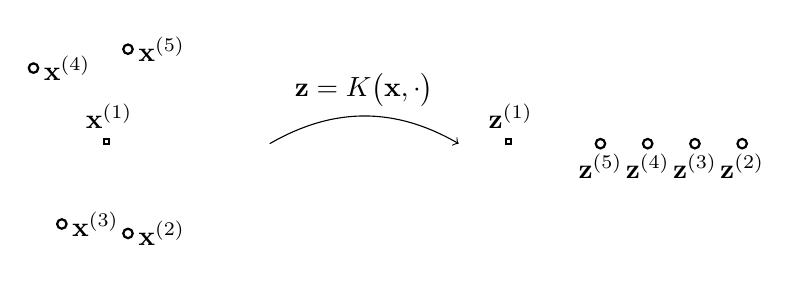
\begin{tikzpicture}[auto,scale=0.6]
        
       
        \draw [thick] (-6,2) circle (0.1cm) node[anchor=west] {\hspace*{0mm}${\bf x}^{(5)}$};
       \draw [thick] (-8,1.6) circle (0.1cm) node[anchor=west] {\hspace*{0mm}${\bf x}^{(4)}$};
        \draw [thick] (-7.4,-1.7) circle (0.1cm) node[anchor=west] {\hspace*{0mm}${\bf x}^{(3)}$};
        \draw [thick] (-6,-1.9) circle (0.1cm) node[anchor=west] {\hspace*{0mm}${\bf x}^{(2)}$};
        \draw [thick] (-6.5,0.0) rectangle ++(0.1cm,0.1cm) node[anchor=west,above] {\hspace*{0mm}${\bf x}^{(1)}$};


      
        \draw [thick] (4,0) circle (0.1cm) node[anchor=north] {\hspace*{0mm}${\bf z}^{(5)}$};
        \draw [thick] (5,0) circle (0.1cm) node[anchor=north] {\hspace*{0mm}${\bf z}^{(4)}$};
        \draw [thick] (6,0) circle (0.1cm) node[anchor=north] {\hspace*{0mm}${\bf z}^{(3)}$};
        \draw [thick] (7,0) circle (0.1cm) node[anchor=north] {\hspace*{0mm}${\bf z}^{(2)}$};
        \draw [thick] (2,0) rectangle ++(0.1cm,0.1cm) node[anchor=west,above] {\hspace*{0mm}${\bf z}^{(1)}$};


       \draw[->,bend left=30] (-3,0) to node[midway,above] {${\bf z} = K\big({\bf x},\cdot\big)$} (1,0);
    \end{tikzpicture}
\end{center}
\caption{
Five data points characterized by feature vectors ${\bf x}^{(r)}$ 
and labels $y^{(r)} \in \{ \circ, \square \}$, for $r=1, \,\ldots, \,5$. 
With these feature vectors, there is no way to separate the two classes 
by a straight line (representing the decision boundary of a linear classifier). 
In contrast, the transformed feature vectors ${\bf z}^{(r)} = K\big({\bf x}^{(r)},\cdot\big)$ 
allow us to separate the data points using a linear classifier.  \label{fig_linsep_kernel_dict}}
\end{figure}
		See also: kernel, feature vector, feature space, linear classifier.},
	first={kernel method},
	text={kernel method} 
}
	

\newglossaryentry{cm}
{name={confusion matrix}, 
	description={Consider data points characterized 
		by features ${\bf x}$ and corresponding labels $y$. 
		The labels take on values in a finite label space $\mathcal{Y} = \{1, \,\ldots, \,k\}$. 
		For a given hypothesis $h$, the confusion matrix is a 
		$k \times k$ matrix where each row corresponds to a different 
		value of the true label $y \in \mathcal{Y}$ and each column to a 
		different value of the prediction $h({\bf x}) \in \mathcal{Y}$. 
		The $(c,c')$th entry of the confusion matrix represents the fraction of 
		data points with a true label $y = c$ that are predicted as 
		$h({\bf x}) = c'$. The main diagonal of the confusion matrix 
		contains the fractions of correctly classified data points (i.e., those for which 
		$y = h({\bf x})$). The off-diagonal entries contain the fractions of
		data points that are misclassified by $h$.
				\\
		See also: label, label space, hypothesis, matrix, classification.},
	first={confusion matrix},
	text={confusion matrix} 
}


\newglossaryentry{featuremtx}
{name={feature matrix}, 
	description={Consider a dataset $\mathcal{D}$ 
		with $m$ data points with feature vectors 
		${\bf x}^{(1)}, \,\ldots, \,{\bf x}^{(m)} \in \mathbb{R}^{d}$. 
		It is convenient to collect the individual feature vectors into a feature 
		matrix ${\bf X} := \big({\bf x}^{(1)}, \,\ldots, \,{\bf x}^{(m)}\big)\,^{T}$ 
		of size $m \times d$.
				\\
		See also: dataset, data point, feature vector, feature, matrix.},
	first={feature matrix},
	text={feature matrix} 
}

\newglossaryentry{dbscan}
{name={density-based spatial clustering of applications with noise (DBSCAN)}, 
	description={DBSCAN 
		refers to a clustering algorithm for data points that are characterized by numeric feature vectors. 
		Like $k$-means and soft clustering via GMM, DBSCAN also uses the Euclidean 
		distances between feature vectors to determine the clusters. However, in contrast to $k$-means 
		and GMM, DBSCAN uses a different notion of similarity between data points. 
		DBSCAN considers two data points as similar if they are connected 
		via a sequence (i.e., path) of nearby intermediate data points. Thus, DBSCAN might consider 
		two data points as similar (and therefore belonging to the same cluster) even if 
		their feature vectors have a large Euclidean distance.
				\\
		See also: clustering, $k$-means, GMM, cluster, graph.},
	first={density-based spatial clustering of applications with noise (DBSCAN)},
	text={DBSCAN} 
}

\newglossaryentry{fl}
{name={federated learning (FL)}, 
	description={FL 
		is an umbrella term for ML methods that train models in a collaborative 
		fashion using decentralized data and computation.
				\\
		See also: ML, model, data.},
	first={federated learning (FL)},
	text={FL} 
}
	
\newglossaryentry{cfl}
{name={clustered federated learning (CFL)}, 
	description={CFL trains local models for the 
 		devices in a FL application by using a clustering assumption, i.e., the devices 
 		of an FL network form clusters. Two devices in the same cluster generate 
 		local datasets with similar statistical properties. CFL pools the local datasets of devices 
 		in the same cluster to obtain a training set for a cluster-specific model. 
 		GTVMin clusters devices implicitly by enforcing approximate similarity of model parameters 
 		across well-connected nodes of the FL network.\\ 
 		See also: FL, clustering assumption, FL network, cluster, graph clustering.},
	first={clustered federated learning (CFL)},
	text={CFL} 
}

\newglossaryentry{iid}
{name={independent and identically distributed (i.i.d.)}, 
	description={A collection of RVs\linebreak ${\bf z}^{(1)}, \,\ldots, \,{\bf z}^{(m)}$ is 
		referred to as i.i.d. 
		if each ${\bf z}^{(r)}$ follows the same probability distribution, and 
		the RVs are mutually independent. That is, for any collection of 
		events $\mathcal{A}_1, \,\ldots, \,\mathcal{A}_m$, we have
       		\[
          		\mathbb{P}({ {\bf z}^{(1)} \in \mathcal{A}_1, \,\ldots, \,{\bf z}^{(m)} \in \mathcal{A}_{m}}) 
         		= \prod_{r=1}^{m} \mathbb{P}({ {\bf z}^{(r)} \in \mathcal{A}_r}).
         	\]
				\\
		See also: RV, probability distribution, event, data point, i.i.d.\ assumption.},
	first={independent and identically distributed (i.i.d.)},
	text={{i.i.d.}} 
}

\newglossaryentry{preimage}
{name={preimage}, 
	description={Consider a function $f\colon \mathcal{U} \rightarrow \mathcal{V}$ 
		between two sets. The preimage $f^{-1}(\mathcal{B})$ of a subset $\mathcal{B} \subseteq \mathcal{V}$ is the set 
		of all inputs $u \in \mathcal{U}$ that are mapped into $\mathcal{B}$ by $f$, i.e.,
		\[
		f^{-1}(\mathcal{B}) := \{ u \in \mathcal{U} \mid f(u) \in \mathcal{B} \}.
		\]
		The preimage is well defined even if the function $f$ is non-invertible \cite{RudinBookPrinciplesMatheAnalysis}.
		\\
		See also: function. },
	first={preimage},
	text={preimage}
}

\newglossaryentry{measurable}
{name={measurable}, 
	description={Consider a random experiment, such as recording the air temperature at an FMI weather station. 
		The corresponding sample space $\Omega$ consists of all possible outcomes $\omega$ (e.g., 
		all possible temperature values in degree Celsius). In many ML applications, we are not interested 
		in the exact outcome $\omega$, but only whether it belongs to a subset $\mathcal{A} \subseteq \Omega$ 
		(e.g., “is the temperature below zero degrees?”). We call such a subset $\mathcal{A}$ measurable if it is 
		possible to decide, for any outcome $\omega$, whether $\omega \in \mathcal{A}$ or not. 
		\begin{figure}[H]
		\begin{center}
		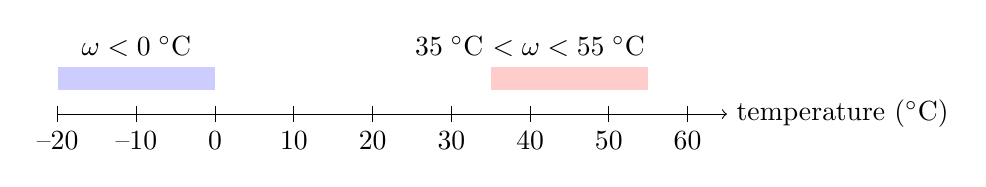
\begin{tikzpicture}
			
			\draw[->] (0,0) -- (8.5,0) node[right] {temperature ($^\circ$C)};
			
			\foreach \x/\label in {0/--20, 1/--10, 2/0, 3/10, 4/20, 5/30, 6/40, 7/50, 8/60} {
				\draw (\x,0.1) -- (\x,-0.1);
				\node[below] at (\x,-0.1) {\label};
			}
			
			\fill[blue!20] (0,0.3) rectangle (2,0.6);
			\node[above] at (1,0.6) {$\omega < 0\;^\circ$C};
			
			\fill[red!20] (5.5,0.3) rectangle (7.5,0.6);
			\node[above] at (6,0.6) {$35\;^\circ$C $< \omega < 55\;^\circ$C};
			\vspace*{10mm}
			\end{tikzpicture}
			\vspace*{10mm}
			\end{center}
			\caption{A sample space constituted by all possible temperature values $\omega$ 
			that may be experienced at an FMI station. Two measurable subsets of temperature 
			values, denoted $\mathcal{A}^{(1)}$ and $\mathcal{A}^{(2)}$, are highlighted. For any 
			actual temperature value $\omega$, it is possible to determine whether $\omega \in \mathcal{A}^{(1)}$ 
			and whether $\omega \in \mathcal{A}^{(2)}$.} 
		\end{figure}
		In principle, measurable sets could be chosen freely (e.g., depending on the resolution of the 
		measuring equipment). However, it is often useful to impose certain completeness requirements 
		on the collection of measurable sets. For example, the sample space itself should be 
		measurable, and the union of two measurable sets should also be measurable. These completeness 
		requirements can be formalized via the concept of $\sigma$-algebra (or $\sigma$-field) 
		\cite{RudinBook}, \cite{BillingsleyProbMeasure}, \cite{durrett2010probability}. 
		A measurable space is a pair $\big(\mathcal{X},\mathcal{F}\big)$ that consists of an arbitrary set $\mathcal{X}$ and a 
		collection $\mathcal{F}$ of measurable subsets of $\mathcal{X}$ that form a $\sigma$-algebra. 
		\\
		See also: sample space, probability.},
	first={measurable},
	text={measurable} 
}

\newglossaryentry{event}
{name={event}, 
	description={Consider an RV ${\bf x}$, defined on some probability space $\mathcal{P}$, 
		which takes values in a measurable space $\mathcal{X}$. An event $\mathcal{A} \subseteq \mathcal{X}$ 
		is a subset of $\mathcal{X}$ such that the probability 
		$\mathbb{P}({{\bf x} \in \mathcal{A}})$ is well defined. In other words, the preimage 
		${\bf x}^{-1}(\mathcal{A})$ of an event belongs to the $\sigma$-algebra of $\mathcal{P}$. 
				\\
		See also: RV, data point, i.i.d.\ assumption, probabilistic model.},
	first={event},
	firstplural={events},
	plural={events},
	text={event} 
}


\newglossaryentry{outlier}
{name={outlier}, 
	description={Many ML methods 
		are motivated by the i.i.d.\ assumption, which interprets data points as realizations of 
		iid RVs with a common probability distribution. The i.i.d.\ assumption is useful for applications  
		where the statistical properties of the data generation process are stationary (or time-invariant) \cite{Brockwell91}. 
		However, in some applications, the data consist of a majority of regular data points 
		that conform with the i.i.d.\ assumption as well as a small number of data points that have fundamentally different 
       		statistical properties compared to the regular data points. We refer to a data point that 
        		substantially deviates from the statistical properties of most data points as an 
        		outlier. Different methods for outlier detection use different measures for this deviation. 
        		Statistical learning theory studies fundamental limits on the ability to mitigate outliers reliably \cite{doi:10.1137/0222052}, \cite{10.1214/20-AOS1961}.
        		\\
		See also: ML, i.i.d.\ assumption, data point, realization, iid, RV, probability distribution, data.},
	 first={outlier},
	 text={outlier} 
}

\newglossaryentry{decisionregion}
{name={decision region}, plural={decision regions}, 
	description={Consider 
		a hypothesis map $h$ that delivers values from a finite set $\mathcal{Y}$. 
		For each label value (i.e., category) $a \in \mathcal{Y}$, the hypothesis $h$ 
		determines a subset of feature values ${\bf x} \in \mathcal{X}$ that result 
		in the same output $h({\bf x})=a$. We refer to this subset as a decision 
		region of the hypothesis $h$.
				\\
		See also: hypothesis, map, label, feature.},
	first={decision region},
	text={decision region} 
}


\newglossaryentry{decisionboundary}
{name={decision boundary}, 
	description={Consider a 
		hypothesis map $h$ that reads in a feature vector  
		${\bf x} \in \mathbb{R}^{d}$ and delivers a value from a finite set $\mathcal{Y}$. 
		The decision boundary of $h$ is the set of vectors ${\bf x} \in \mathbb{R}^{d}$ 
		that lie between different decision regions. More precisely, a 
		vector ${\bf x}$ belongs to the decision boundary if and only 
		if each neighborhood $\{ {\bf x}': \| {\bf x} - {\bf x}' \| \leq \varepsilon \}$, 
		for any $\varepsilon >0$, contains at least two vectors with different function values.
				\\
		See also: hypothesis, map, feature vector, vector, decision region, neighborhood, function.},
	first={decision boundary},
	text={decision boundary} 
}


\newglossaryentry{euclidspace}
{name={Euclidean space}, 
	description={The 
		Euclidean space $\mathbb{R}^{d}$ of dimension $d \in \mathbb{N}$ consists 
		of vectors ${\bf x}= \big(x_{1}, \,\ldots, \,x_{d}\big)$, with $d$ 
		real-valued entries $x_{1}, \,\ldots, \,x_{d} \in \mathbb{R}$. Such a Euclidean 
		space is equipped with a geometric structure defined by the inner product 
		${\bf x}\,^{T} {\bf x}' = \sum_{j=1}^{d} x_{j} x'_{j}$ 
		between any two vectors ${\bf x},{\bf x}' \in \mathbb{R}^{d}$ \cite{RudinBookPrinciplesMatheAnalysis}.
		\\
		See also: vector. },
	first={Euclidean space},
	text={Euclidean space} 
}

\newglossaryentry{eerm}
{name={explainable empirical risk minimization (EERM)}, 
	description={EERM is an 
		in-\linebreak stance of SRM that adds a regularization term to the 
		average loss in the objective function of ERM. 
		The regularization term is chosen to favor hypothesis maps that are intrinsically 
		explainable for a specific user. This user is characterized by their predictions provided 
		for the data points in a training set \cite{Zhang:2024aa}.
				\\
		See also: SRM, regularization, loss, objective function, ERM, hypothesis, map, prediction, data point, training set.},
	first={explainable empirical risk minimization (EERM)},
	text={EERM} 
}
	
	
\newglossaryentry{kmeans}
{name={$k$-means}, 
sort={k-means},
	description={The $k$-means algorithm 
		is a hard clustering method that assigns each data point of a dataset 
		to precisely one of $k$ different clusters. The method alternates between updating 
		the cluster assignments (to the cluster with the nearest mean) and 
		recalculating the cluster means given the updated cluster assignments \cite[Ch. 8]{MLBasics}.
				\\
		See also: hard clustering, cluster.},
	first={$k$-means},
	text={$k$-means} 
}


\newglossaryentry{xml}
{name={explainable machine learning (XML)}, 
	description={XML 
		methods aim to complement each prediction with an explanation of 
		how the prediction has been obtained. The construction of an explicit explanation 
		might not be necessary if the ML method uses a sufficiently simple (or interpretable) model \cite{rudin2019stop}.
				\\
		See also: prediction, explanation, ML, model.},
	first={XML},
	text={XML} 
}

\newglossaryentry{fmi}
{name={Finnish Meteorological Institute (FMI)}, 
	description={The
		FMI is a government agency responsible for gathering 
		and reporting weather data in Finland.
				\\
		See also: data.},
	first={Finnish Meteorological Institute (FMI)},
	text={FMI} 
}
	
	
\newglossaryentry{samplemean}
{name={sample mean}, 
	description={The sample mean 
		${\bf m} \in \mathbb{R}^{d}$ for a given dataset, with feature vectors 
		${\bf x}^{(1)}, \,\ldots, \,{\bf x}^{(m)} \in \mathbb{R}^{d}$, is defined as 
		$${\bf m} = \frac{1}{m} \sum_{r=1}^{m} {\bf x}^{(r)}.$$ 
					\\
		See also: sample, mean, dataset, feature vector.},
	first={sample mean},
	text={sample mean} 
}

	
\newglossaryentry{samplecovmtx}
{name={sample covariance matrix}, 
	description={The 
		sample covariance matrix $\widehat{\bf \Sigma} \in \mathbb{R}^{d \times d}$ 
		for a given set of feature vectors ${\bf x}^{(1)}, \,\ldots, \,{\bf x}^{(m)} \in \mathbb{R}^{d}$ is defined as 
		$$\widehat{\bf \Sigma} = \frac{1}{m} \sum_{r=1}^{m} ({\bf x}^{(r)}\!-\!\widehat{{\bf m}}) ({\bf x}^{(r)}\!-\!\widehat{{\bf m}})\,^{T}.$$ 
		Here, we use the sample mean $\widehat{{\bf m}}$. 
				\\
		See also: sample, covariance matrix, feature vector, sample mean.},
	first={sample covariance matrix},
	text={sample covariance matrix} 
}

\newglossaryentry{covmtx}
{name={covariance matrix}, 
	description={The covariance matrix of an RV ${\bf x} \in \mathbb{R}^{d}$ 
		is defined as $\mathbb{E}  \bigg \{ \big( {\bf x} - \mathbb{E}  \big\{ {\bf x} \big\} \big)  \big({\bf x} - \mathbb{E}  \big\{ {\bf x} \big\} \big)\,^{T} \bigg\}$.
				\\
		See also: covariance, matrix, RV.},
	first={covariance matrix},
	text={covariance matrix} 
}
	
\newglossaryentry{highdimregime}
{name={high-dimensional regime}, 
	description={The 
		high-dimensional regime of ERM is characterized by the effective dimension of the model 
		being larger than the sample size, i.e., the number of (labeled) data points in the training set. 
		For example, linear regression methods operate in the high-dimensional regime whenever the number $d$ of features 
		used to characterize data points exceeds the number of data points in the training set. 
		Another example of ML methods that operate in the high-dimensional regime is large ANNs, which have 
		far more tunable weights (and bias terms) than the total number of data points in the training set. 
		High-dimensional statistics is a recent main thread of probability theory that studies the 
		behavior of ML methods in the high-dimensional regime \cite{Wain2019}, \cite{BuhlGeerBook}.
				\\
		See also: ERM, effective dimension, overfitting, regularization.},
   	first={high-dimensional regime},
	text={high-dimensional regime} 
}

\newglossaryentry{covariance}
{name={covariance}, 
	description={The covariance between two real-valued 
 		RVs $x$ and $y$, defined on a common probability space, measures their linear 
 		dependence. It is defined as 
			$$
			{\rm cov}\left(x,y\right) = \mathbb{E} \big\{ \big(x - \mathbb{E} \{ x\} \big)\big(y - \mathbb{E} \{y\} \big)\big\}.
			$$
		A positive covariance indicates that $x$ and $y$ tend to increase together, 
		while a negative covariance suggests that one tends to increase as the other decreases. 
		If ${\rm cov}\left(x,y\right) = 0$, the RVs are said to be uncorrelated, though not necessarily statistically 
		independent. See Fig. \ref{fig:covariance-examples_dict} for visual illustrations.
		\begin{figure}[H]
		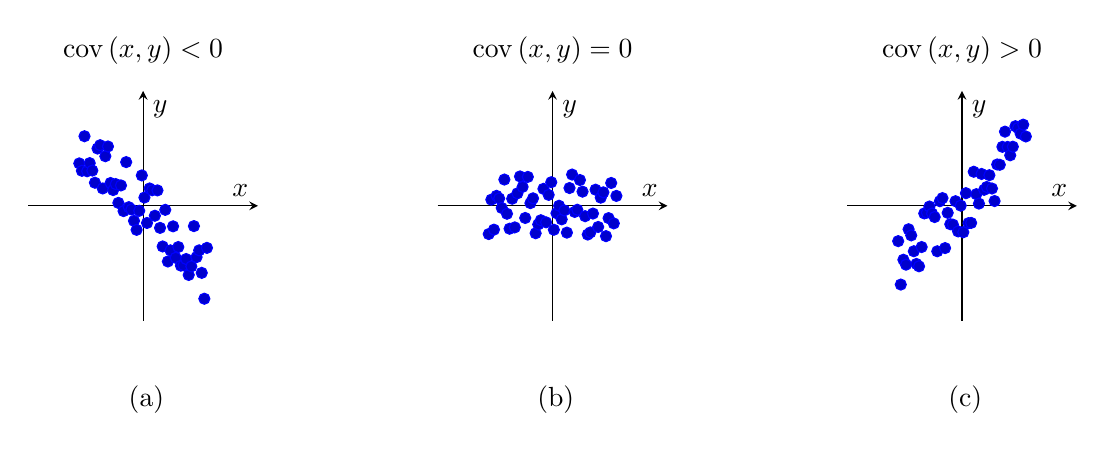
\begin{tikzpicture}
		
		\begin{scope}[shift={(0,0)}]
			\begin{axis}[
				width=4.5cm, height=4.5cm,
				title={${\rm cov}\left(x,y\right) <0$},
				xlabel={$x$}, ylabel={$y$},
				xmin=-3, xmax=3, ymin=-3, ymax=3,
				xtick=\empty, ytick=\empty,
				axis lines=middle, enlargelimits
				]
				\addplot+[only marks, mark=*, samples=50, domain=-2:2] 
				({x}, {-x + rand});
			\end{axis}
			\node at (1.5,-1) {(a)};
		\end{scope}
		
		\begin{scope}[shift={(5.2cm,0)}]
			\begin{axis}[
				width=4.5cm, height=4.5cm,
				title={${\rm cov}\left(x,y\right) =0$}, 
				xlabel={$x$}, ylabel={$y$},
				xmin=-3, xmax=3, ymin=-3, ymax=3,
				xtick=\empty, ytick=\empty,
				axis lines=middle, enlargelimits
				]
				\addplot+[only marks, mark=*, samples=50, domain=-2:2] 
				({x}, {rand});
			\end{axis}
			\node at (1.5,-1) {(b)};
		\end{scope}
		
		\begin{scope}[shift={(10.4cm,0)}]
			\begin{axis}[
				width=4.5cm, height=4.5cm,
				title={${\rm cov}\left(x,y\right) > 0$},
				xlabel={$x$}, ylabel={$y$},
				xmin=-3, xmax=3, ymin=-3, ymax=3,
				xtick=\empty, ytick=\empty,
				axis lines=middle, enlargelimits
				]
				\addplot+[only marks, mark=*, samples=50, domain=-2:2] 
				({x}, {x + rand});
			\end{axis}
			\node at (1.5,-1) {(c)};
		\end{scope}
		\end{tikzpicture}
			\caption{Scatterplots illustrating realizations from three different probabilistic models for two 
				RVs with different covariance values. (a) Negative. (b) Zero. (c) Positive.}
			\label{fig:covariance-examples_dict}
		\end{figure}
		See also: probabilistic model, expectation. },
	first={covariance},
	text={covariance} 
}

\newglossaryentry{gmm}
{name={Gaussian mixture model (GMM)}, 
	description={A GMM 
		is a particular type of probabilistic model for a numeric vector ${\bf x}$ (e.g., 
		the features of a data point). Within a GMM, the vector ${\bf x}$ is drawn from a randomly 
		selected multivariate normal distribution $p^{(c)} = \mathcal{N}\left({\bm \mu}^{(c)},\mathbf{C}^{(c)}\right)$ with 
		$c = I$. The index $I \in \{1, \,\ldots, \,k\}$ is an RV with probabilities $\mathbb{P}({I=c}) = p_{c}$.
	     	Note that a GMM is parameterized by the probability $p_{c}$, the 
		mean vector ${\bm \mu}^{(c)}$, and the covariance matrix $\mathbf{C}^{(c)}$ for each $c=1, \,\ldots, \,k$. 
		GMMs are widely used for clustering, density estimation, and as a generative model. 
				\\
		See also: probabilistic model, multivariate normal distribution, clustering.},
	first={Gaussian mixture model (GMM)},
	text={GMM} 
}
 
\newglossaryentry{maxlikelihood}
{name={maximum likelihood}, 
	description={Consider data points $\mathcal{D}=\big\{ {\bf z}^{(1)}, \,\ldots, \,{\bf z}^{(m)} \}$ 
		that are interpreted as the realizations of iid RVs with a common probability distribution $\mathbb{P}({{\bf z}; {\bf w}})$, which 
		depends on the model parameters ${\bf w} \in \mathcal{W} \subseteq \mathbb{R}^{n}$. 
		Maximum likelihood methods learn model parameters ${\bf w}$ by maximizing 
		the probability (density) $\mathbb{P}({\mathcal{D}; {\bf w}}) = \prod_{r=1}^{m} \mathbb{P}({{\bf z}^{(r)}; {\bf w}})$ 
		of the observed dataset. Thus, the maximum likelihood estimator is a 
		solution to the optimization problem $\max_{{\bf w} \in \mathcal{W}} \mathbb{P}({\mathcal{D}; {\bf w}})$.
				\\
		See also: probability distribution, optimization problem, probabilistic model.},
	first={maximum likelihood},
	text={maximum likelihood}
}


\newglossaryentry{em}
{name={expectation–maximization (EM)}, 
	description={ 
		Consider a probabilistic model $\mathbb{P}({{\bf z}; {\bf w}})$ for the data points $\mathcal{D}$ generated in some 
		ML application. The maximum likelihood estimator for the model parameters ${\bf w}$ is obtained by maximizing 
		$\mathbb{P}({\mathcal{D}; {\bf w}})$. However, the resulting optimization problem might be computationally 
		challenging. EM approximates the maximum likelihood estimator by introducing a latent 
		RV ${\bf z}$ such that maximizing $\mathbb{P}({\mathcal{D},{\bf z}; {\bf w}})$ would be easier 
		\cite{hastie01statisticallearning}, \cite{BishopBook}, \cite{GraphModExpFamVarInfWainJor}. Since we 
		do not observe ${\bf z}$, we need to estimate it from the observed dataset $\mathcal{D}$ 
		using a conditional expectation. The resulting estimate $\widehat{{\bf z}}$ is then used to 
		compute a new estimate $\widehat{{\bf w}}$ by solving $\max_{{\bf w}} \mathbb{P}({\mathcal{D}, \widehat{{\bf z}}; {\bf w}})$. 
		The crux is that the conditional expectation $\widehat{{\bf z}}$ depends on the model parameters $\widehat{{\bf w}}$, 
		which we have updated based on $\widehat{{\bf z}}$. Thus, we have to recalculate $\widehat{{\bf z}}$, 
		which, in turn, results in a new choice $\widehat{{\bf w}}$ for the model parameters. In practice, 
		we repeat the computation of the conditional expectation (i.e., the E-step) and the update 
		of the model parameters (i.e., the M-step) until some stopping criterion is met. 
				\\
		See also: probabilistic model, maximum likelihood, optimization problem. },
	first={EM},
	text={EM}
}


\newglossaryentry{ppca}
{name={probabilistic principal component analysis (PPCA)}, 
	description={PPCA 
		extends\linebreak basic PCA by using a probabilistic model for data points. 
		The probabilistic model of PPCA reduces the task of dimensionality reduction 
		to an estimation problem that can be solved using EM \cite{TippingProbPCA}.
				\\
		See also: PCA, probabilistic model, dimensionality reduction, EM.},
	first={probabilistic principal component analysis (PPCA)},
	text={PPCA}
}
	
\newglossaryentry{polyreg}
{name={polynomial regression}, 
	description={Polynomial 
		regression is an instance of ERM that learns a polynomial hypothesis 
		map to predict a numeric label based on the numeric features of a data point. 
		 For data points characterized by a single numeric feature, polynomial regression uses the hypothesis space 
		$\mathcal{H}^{(\rm poly)}_{d} := \{ h(x) = \sum_{j=0}^{d-1} x^{j} w_{j} \}.$
		The quality of a polynomial hypothesis map is measured using the average squared error loss 
		incurred on a set of labeled data points (which we refer to as the training set).
					\\
		See also: regression, ERM, squared error loss.},
	first={polynomial regression},
	text={polynomial regression}
}

\newglossaryentry{linreg}
{name={linear regression}, 
	description={Linear 
		regression aims to learn a linear hypothesis map to predict a numeric label based 
		on the numeric features of a data point. The quality of a linear hypothesis map is 
		measured using the average squared error loss incurred on a set of labeled data points, 
		which we refer to as the training set.
				\\
		See also: regression, hypothesis, map, label, feature, data point,  squared error loss, labeled data point, training set.},
	first={linear regression},
	text={linear regression}
}
        
\newglossaryentry{ridgeregression}
{name={ridge regression}, 
	description={Consider a regression problem where the goal is to learn a hypothesis $h^{({\bf w})}$ 
		for predicting the numeric label of a data point based on its feature vector. 
	  	Ridge regression learns the parameters ${\bf w}$ 
	  	by minimizing the penalized average squared error loss. The average squared error loss is measured 
		on a set of labeled data points (i.e., the training set) 
		$$\left( {\bf x}^{(1)},y^{(1)} \right), \,\ldots, \,\left( {\bf x}^{(m)},y^{(m)} \right).$$ 
		The penalty term is the scaled squared Euclidean norm $\alpha \| {\bf w} \|^{2}_{2}$ with a 
		regularization parameter $\alpha > 0$. The purpose of the penalty term is regularization, 
		i.e., to prevent overfitting in the high-dimensional regime, where the number of features 
		$d$ exceeds the number of data points $m$ in the training set.
		Adding $\alpha \| {\bf w} \|^{2}_{2}$ to the average squared error loss is equivalent 
		to computing the average squared error loss on an augmented training set. This augmented 
		training set is obtained by replacing each data point $\left( {\bf x}^{(r)},y^{(r)} \right)$ 
		in the original training set by the realization of infinitely many iid RVs 
		whose probability distribution is centered at $\left( {\bf x}^{(r)},y^{(r)} \right)$.
	    		\\
		See also: regression, regularization, map, data augmentation.},
	first={ridge regression},
	text={ridge regression}
}


\newglossaryentry{expectation}
{name={expectation}, plural={expectations},
  description={Consider a numeric feature vector ${\bf x} \in \mathbb{R}^{d}$ 
	that we interpret as the realization of an RV with a probability distribution $p({\bf x})$. 
	The expectation of ${\bf x}$ is defined as the integral $\mathbb{E}  \{ {\bf x} \} := \int {\bf x} p({\bf x})$. 
	Note that the expectation is only defined if this integral exists, i.e., if the RV is integrable 
	\cite{RudinBookPrinciplesMatheAnalysis}, \cite{BillingsleyProbMeasure}, \cite{HalmosMeasure}. 
	Fig. \ref{fig_expect_discrete_dict} illustrates the expectation of a scalar discrete RV $x$ that takes on values 
	from a finite set only. 
   \begin{figure}[H]
   	\begin{center}
   	\begin{tikzpicture}
\begin{axis}[
	ybar,
	y=5cm,
	x=2cm,                          
	bar width=0.6cm,                   

	xlabel={$x_i$},
	clip=false,
	ylabel={$p(x_i)$},
	y label style={rotate=-90, anchor=west, xshift=-1cm},
	xtick={1,2,3,4,5},
	ymin=0, ymax=0.6,
	grid=both,
	major grid style={gray!20},
	tick align=outside,
	axis line style={black!70},
	]
	\addplot+[ybar, fill=blue!50] coordinates {
		(1,0.1) 
		(2,0.2) 
		(3,0.4) 
		(4,0.2)
		(5,0.1)
	};
	
	\node[font=\footnotesize,xshift=7pt] at (axis cs:1,0.13) {$p(x_i)\!\,\cdot\!\,x_i\!=\!0.1$};
	\node[font=\footnotesize]at (axis cs:2,0.23) {$0.4$};
	\node[font=\footnotesize]at (axis cs:3,0.43) {$1.2$};
	\node[font=\footnotesize] at (axis cs:4,0.23) {$0.8$};
	\node[font=\footnotesize]at (axis cs:5,0.13) {$0.5$};
	\node[font=\footnotesize]at (axis cs:3.8,0.53) {$\mathbb{E} \{x\}\!=\!0.1\!+\!0.4\!+\!1.2\!+\!0.8\!+\!0.5\!=\!3$};
\end{axis}
\end{tikzpicture}
\end{center}
\vspace*{-5mm}
\caption{The expectation of a discrete RV $x$ is obtained by summing its possible values $x_{i}$, weighted 
	by the corresponding probability $p(x_i) = \mathbb{P}({x= x_i})$. \label{fig_expect_discrete_dict}}
 \end{figure}
		See also: feature vector, realization, RV, probability distribution, probability.},
first={expectation},
text={expectation}
}

\newglossaryentry{logreg}
{name={logistic regression}, 
	description={Logistic regression learns a 
		linear hypothesis map (or classifier) $h({\bf x}) = {\bf w}\,^{T} {\bf x}$ 
		to predict a binary label $y$ based on the numeric feature vector ${\bf x}$ of 
		a data point. The quality of a linear hypothesis map is measured by the average logistic loss 
		on some labeled data points (i.e., the training set).
				\\
		See also: regression, hypothesis, map, classifier, label, feature vector, data point, logistic loss, labeled data point, training set.},
	first={logistic regression},
	text={logistic regression}
}
	
\newglossaryentry{logloss}
{name={logistic loss}, 
	description={Consider 
		a data point characterized by the features ${\bf x}$ and a binary label $y \in \{-1,1\}$. 
		We use a real-valued hypothesis $h$ to predict the label $y$ 
		from the features ${\bf x}$. The logistic loss incurred by this prediction is 
		defined as 
	\begin{equation} 
		\label{equ_log_loss_gls_dict}
		L\left(({\bf x},y),h \right) :=  \log\, ( 1 + \exp\,(- y h({\bf x}))).
	\end{equation}
	\begin{figure}[H]
	\begin{center}
		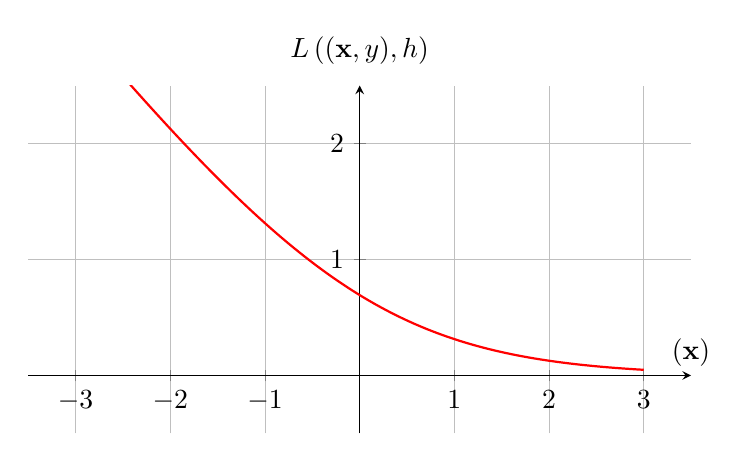
\begin{tikzpicture}
			\begin{axis}[
				axis lines=middle,
				xlabel={$\truelabelh({\bf x})$},
				ylabel={$L\left(({\bf x},y),h \right)$},
				xlabel style={at={(axis description cs:1.,0.3)}, anchor=north},  
				ylabel style={at={(axis description cs:0.5,1.1)}, anchor=center}, 
				xmin=-3.5, xmax=3.5,
				ymin=-0.5, ymax=2.5,
				xtick={-3, -2, -1, 0, 1, 2, 3},
				ytick={0, 1, 2},
				domain=-3:3,
				samples=100,
				width=10cm, height=6cm,
				grid=both,
				major grid style={line width=.2pt, draw=gray!50},
				minor grid style={line width=.1pt, draw=gray!20},
				legend pos=south west 
				]
					\addplot [red, thick] {ln(1 + exp(-x))};    
			\end{axis}
		\end{tikzpicture}
		\caption{The logistic loss incurred by the prediction $h({\bf x}) \in \mathbb{R}$ 
			for a data point with label $y \in \{-1,1\}$.}
		\label{fig_logloss_dict}
	\end{center}
	\end{figure}
	Note that the expression \eqref{equ_log_loss_gls_dict} 
	for the logistic loss applies only for the label space $\mathcal{Y} = \{ -1,1\}$ and when using 
	the thresholding rule \eqref{equ_def_threshold_bin_classifier_dict}. 
		\\
		See also: data point, feature, label, hypothesis, loss, prediction, label space.},
	first={logistic loss},
	text={logistic loss}
}
	
\newglossaryentry{hingeloss}
{name={hinge loss}, 
	description={Consider a data point 
		characterized by a feature vector ${\bf x} \in \mathbb{R}^{d}$ and a 
		binary label $y \in \{-1,1\}$. The hinge loss incurred by a real-valued 
		hypothesis map $h({\bf x})$ is defined as 
		\begin{equation} 
			\label{equ_hinge_loss_gls_dict}
				L\left(({\bf x},y),h \right) := \max \{ 0 , 1 - y h({\bf x}) \}. 
			\end{equation}
\begin{figure}[H]
\begin{center}
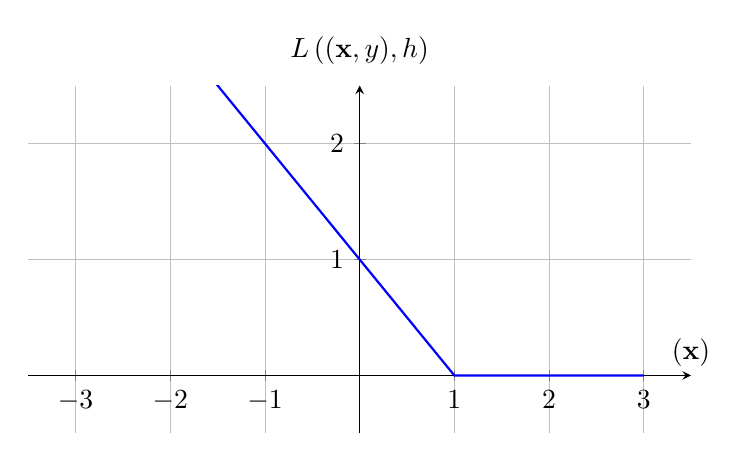
\begin{tikzpicture}
    \begin{axis}[
        axis lines=middle,
        xlabel={$\truelabelh({\bf x})$},
        ylabel={$L\left(({\bf x},y),h \right)$},
 	xlabel style={at={(axis description cs:1.,0.3)}, anchor=north},  
        ylabel style={at={(axis description cs:0.5,1.1)}, anchor=center}, 
        xmin=-3.5, xmax=3.5,
        ymin=-0.5, ymax=2.5,
        xtick={-3, -2, -1, 0, 1, 2, 3},
        ytick={0, 1, 2},
        domain=-3:3,
        samples=100,
        width=10cm, height=6cm,
        grid=both,
        major grid style={line width=.2pt, draw=gray!50},
        minor grid style={line width=.1pt, draw=gray!20},
        legend pos=south west 
    ]
        \addplot[blue, thick] {max(0, 1-x)};
     
    \end{axis}
\end{tikzpicture}
\caption{The hinge loss incurred by the prediction $h({\bf x}) \in \mathbb{R}$ 
for a data point with label $y \in \{-1,1\}$. A regularized variant of the hinge 
loss is used by the SVM \cite{LampertNowKernel}.}
\label{fig_hingeloss_dict}
\end{center}
\end{figure} 	    
		See also: data point, feature vector, label, loss, hypothesis, map, prediction, SVM.},
	first={hinge loss},
	text={hinge loss}
}

\newglossaryentry{iidasspt}
{name={independent and identically distributed assumption (i.i.d.\ assumption)}, 
	description={The iid assumption interprets data points of a dataset as the 
		realizations of iid RVs.
				\\
		See also: iid, data point, dataset, realization, RV.},
	first={independent and identically distributed assumption (i.i.d.\ assumption)},
	text={i.i.d.\ assumption} 
}

\newglossaryentry{hypospace}
{name={hypothesis space}, plural={hypothesis spaces}, 
	description={A hypothesis space is a mathematical model 
		that characterizes the learning capacity of an ML method. The goal of such a method is 
		to learn a hypothesis map that maps features of a data point to a 
		prediction of its label. Given a finite amount of computational resources, a 
		practical ML method typically explores only a restricted set of all possible maps 
		from the feature space to the label space. Such a restricted set is referred to as 
		a hypothesis space $\mathcal{H}$ underlying the ML method.
    		For the analysis of a given ML method, the choice of a hypothesis space $\mathcal{H}$ is not 
		unique, i.e., any superset containing all maps the method can learn is also a valid hypothesis space. 
		\begin{figure}[H]
		\begin{center}
			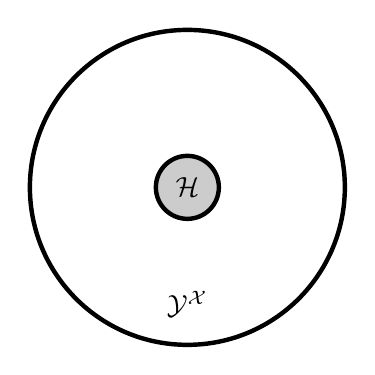
\begin{tikzpicture}[allow upside down, scale=0.4]
			\node [below] at (5,-3) {$\mathcal{Y}^{\mathcal{X}}$};
			\draw [ultra thick] (5,0) circle (5cm);
			\draw [ultra thick,fill=black!20] (5,0) circle (1cm);
			\node [] at (5,0) {$\mathcal{H}$};
			\end{tikzpicture}
		\end{center}
		\caption{The hypothesis space $\mathcal{H}$ of an ML method is a (typically very small) 
		subset of the (typically very large) set $\mathcal{Y}^{\mathcal{X}}$ of all possible maps 
		from the feature space $\mathcal{X}$ into the label space $\mathcal{Y}$.}
		\end{figure}
		On the other hand, from an ML engineering perspective, the hypothesis space $\mathcal{H}$ is a design 
		choice for ERM-based methods. This design choice can be guided by the available computational 
		resources and statistical aspects. For instance, if efficient matrix operations are feasible and a 
		roughly linear relation exists between features and labels, a linear model can be a 
		useful choice for $\mathcal{H}$.
				\\
		See also: hypothesis, model, map, linear model.},
	first={hypothesis space},
	text={hypothesis space} 
}

	
\newglossaryentry{model}
{name={model}, plural={models}, 
	description={The study and design of ML methods is often based on a mathematical model \cite{bender1978mathematical}. 
		Maybe the most widely used example of a mathematical model for ML is a hypothesis space. 
		A hypothesis space consists of hypothesis maps that are used by an ML method to 
		predict labels from the features of data points. Another important type of 
		mathematical model is a probabilistic model, which consists of probability distributions that describe 
		how data points are generated. Unless stated otherwise, we use the term model to 
		refer specifically to the hypothesis space underlying an ML method. 
		\begin{figure}[H]
			\centering
			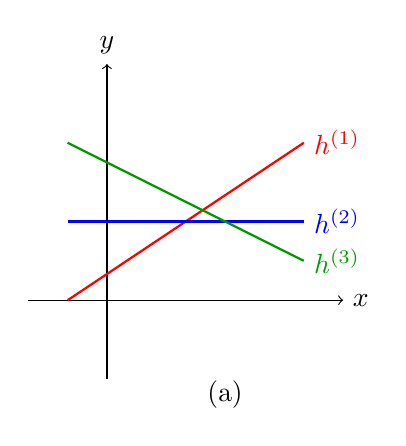
\begin{tikzpicture}[scale=1]
			\draw[->] (-1,0) -- (3,0) node[right] {$x$};
			\draw[->] (0,-1) -- (0,3) node[above] {$y$};
			\draw[thick, red] (-0.5,0) -- (2.5,2) node[right] {$h^{(1)}$};
			\draw[thick, blue] (-0.5,1) -- (2.5,1) node[right] {$h^{(2)}$};
			\draw[thick, green!60!black] (-0.5,2) -- (2.5,0.5) node[right] {$h^{(3)}$};
			\node at (1.5,-1.2) {(a)};
			\end{tikzpicture}
			\hspace{2cm}
			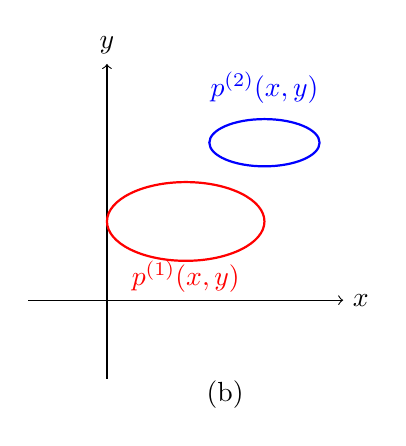
\begin{tikzpicture}[scale=1]
			\draw[->] (-1,0) -- (3,0) node[right] {$x$};
			\draw[->] (0,-1) -- (0,3) node[above] {$y$};
			\draw[thick, red] (1,1) ellipse [x radius=1, y radius=0.5];
			\draw[thick, blue] (2,2) ellipse [x radius=0.7, y radius=0.3];
			\node[red] at (1,0.3) {$p^{(1)}(x,y)$};
			\node[blue] at (2,2.7) {$p^{(2)}(x,y)$};
			\node at (1.5,-1.2) {(b)};
			\end{tikzpicture}
		\caption{Two types of mathematical models used in ML. (a) A hypothesis space consisting of 
		three linear maps. (b) A probabilistic model consisting of probability distribution over the plane spanned by 
		the feature and label values of a data point.}
		\end{figure}
		See also: hypothesis space, probabilistic model, probability distribution.},
	first={model},
	text={model} 
}

\newglossaryentry{modelparams}
{name={model parameters}, 
	description={Model parameters are quantities that 
		are used to select a specific hypothesis map from a model. 
		We can think of a list of model parameters as a unique identifier for a hypothesis 
		map, similar to how a social security number identifies a person in Finland.
			\\
		See also: model, parameter, hypothesis, map.},
	first={model parameters},
	text={model parameters} 
}

\newglossaryentry{ai}
{name={artificial intelligence (AI)}, 
	description={AI refers to systems that behave rationally in the sense of 
		maximizing a long-term reward. The ML-based approach to AI is to train a model to  
		predict optimal actions. These predictions are computed from observations about the state of the 
		environment. The choice of loss function sets AI applications apart from more basic ML applications. 
		AI systems rarely have access to a labeled training set that allows the average loss to be 
		measured for any possible choice of model parameters. Instead, AI systems use observed reward 
		signals to estimate the loss incurred by the current choice of model parameters.
				\\
		See also: ML, RL.},
	first={AI},
	text={AI} 
}


\newglossaryentry{mdp}
{name={Markov decision process (MDP)},
	description={An MDP  is a mathematical structure that can 
    		be used to study RL applications. An MDP formalizes how reward 
		signals depend on the predictions (and corresponding actions) made by an RL 
		method. Formally, an MDP is a specific type of stochastic process defined by
		\begin{itemize}
    			\item a state space $\mathcal{S}$;
    			\item an action space $\mathcal{A}$ (where each action $a \in \mathcal{A}$ corresponds to a specific 
			prediction made by the RL method);
    			\item a transition function $\mathbb{P}({s' \mid s, a})$ specifying the probability distribution over the 
			next state $s' \in \mathcal{S}$, given the current state $s \in \mathcal{S}$ and action $a \in \mathcal{A}$;
    			\item a reward function $r(s, a) \in \mathbb{R}$ that assigns a numerical reward to each 
			state-action pair.
		\end{itemize}
		The defining property of an MDP is the Markov property. That is, the next state $s'$ and reward 
		only depend on the current state $s$ and action $a$, not on the entire history of interactions. 
		\\
		See also: RL, reward, prediction, stochastic process, function, probability distribution.},
 	first={mdp},
 	text={mdp} 
 }
 

\newglossaryentry{reward}
{name={reward}, 
	description={A reward refers to some observed 
		(or measured) quantity that allows us to estimate the loss incurred by the prediction 
		(or decision) of a hypothesis $h({\bf x})$. For example, in an 
		ML application to self-driving vehicles, $h({\bf x})$ could represent 
		the current steering direction of a vehicle. We could construct a reward from the 
		measurements of a collision sensor that indicate if the vehicle is moving toward 
		an obstacle. We define a low reward for the steering direction 
		$h({\bf x})$ if the vehicle moves dangerously toward an obstacle.
			\\
		See also: loss, MAB, RL.},
	first={reward}, 
	text={reward}
} 

\newglossaryentry{hardclustering}
{name={hard clustering}, 
	description={Hard clustering 
		refers to the task of partitioning a given set of data points into (a few) nonoverlapping clusters. 
		The most widely used hard clustering method is $k$-means.
				\\
		See also: clustering, data point, cluster, $k$-means.},
	first={hard clustering},
	text={hard clustering} 
}
	
\newglossaryentry{softclustering}
{name={soft clustering}, 
	description={Soft clustering 
		refers to the task of partitioning a given set of data points into (a few) overlapping clusters. 
		Each data point is assigned to several different clusters with varying degrees of belonging. Soft clustering 
		methods determine the degree of belonging (or soft cluster assignment) for each data point and each cluster.
		A principled approach to soft clustering is by interpreting data points as iid realizations 
		of a GMM. We then obtain a natural choice for the degree of belonging as the conditional 
		probability of a data point belonging to a specific mixture component.
				\\
		See also: clustering, data point, cluster, degree of belonging, iid, realization, GMM, probability.},
	first={soft clustering},
	text={soft clustering} 
}

\newglossaryentry{kroneckerproduct}
{name={Kronecker product}, 
	description={The Kronecker product  of two matrices ${\bf A} \in \mathbb{R}^{m \times n}$ 
		and ${\bf B} \in \mathbb{R}^{p \times q}$ is a block matrix denoted ${\bf A} \otimes {\bf B}$ 
	 	and defined as \cite{GolubVanLoanBook}, \cite{HornMatAnalysis}
    		\[
      		{\bf A} \otimes {\bf B} =
      		\begin{bmatrix}
        		a_{11}{\bf B} & \cdots & a_{1n}{\bf B} \\
        		\vdots & \ddots & \vdots \\
        		a_{m1}{\bf B} & \cdots & a_{mn}{\bf B}
      		\end{bmatrix}
      		\in \mathbb{R}^{mp \times nq}.
    		\]
    		The Kronecker product is a special case of the tensor product for matrices and is 
		widely used in multivariate statistics, linear algebra, and structured ML models. 
		It satisfies the identity $({\bf A} \otimes {\bf B})({\bf x} \otimes {\bf y}) = ({\bf A}{\bf x}) \otimes ({\bf B}{\bf y})$ 
		for vectors ${\bf x}$ and ${\bf y}$ of compatible dimensions.
		\\
		See also: matrix, ML, model, vector. },
	first={Kronecker product},
	text={Kronecker product} 
}
	
\newglossaryentry{clustering}
{name={clustering}, 
	description={Clustering methods decompose a given 
		set of data points into a few subsets, which are referred to as clusters. 
		Each cluster consists of data points that are more similar to each 
		other than to data points outside the cluster. Different clustering methods 
		use different measures for the similarity between data points and different 
		forms of cluster representations. The clustering method $k$-means uses the 
		average feature vector of a cluster (i.e., the cluster mean) as its representative. 
		A popular soft clustering method based on GMM represents 
		a cluster by a multivariate normal distribution.
				\\
		See also: cluster, $k$-means, soft clustering, GMM.},
	first={clustering},
	text={clustering} 
}
	
\newglossaryentry{cluster}
{name={cluster}, plural={clusters}, 
	description={A cluster is a subset of 
		data points that are more similar to each other than to the data points outside the cluster. 
		The quantitative measure of similarity between data points is a design choice. If data points 
		are characterized by Euclidean feature vectors ${\bf x} \in \mathbb{R}^{d}$, 
		we can define the similarity between two data points via the Euclidean distance between 
		their feature vectors. An example of such clusters is shown in Fig. \ref{fig:clusters_dict}.\\
		\begin{figure}[H]
		\centering
		\begin{tikzpicture}
		\pgfplotsset{compat=1.18}
		\begin{axis}[
		    width=10cm,
		    height=8cm,
		    xlabel={$x_1$},
		    ylabel={$x_2$},
		    title={Clusters of Data Points},
		    xmin=0, xmax=10,
		    ymin=0, ymax=10,
		    axis lines=left,
		    legend style={at={(0.5,-0.25)}, anchor=north, legend columns=3}
		]
		
		\addplot[only marks, color=blue, mark=*, mark size=3pt] coordinates {
		    (1,1) (2,1.2) (1.8,2) (2.2,1.5) (1.5,2.5)
		};
		
		\addplot[only marks, color=red, mark=square*, mark size=3pt] coordinates {
		    (7,8) (8,7.5) (7.5,8.5) (8.2,7.8) (7.7,7)
		};
		
		\addplot[only marks, color=green!60!black, mark=triangle*, mark size=3pt] coordinates {
		    (5,3) (5.5,3.2) (5.2,2.8) (4.8,3.5) (5.1,3.1)
		};
		\legend{Cluster 1, Cluster 2, Cluster 3}
		\end{axis}
		\end{tikzpicture}
		\caption{Illustration of three clusters in a 2-D feature space. Each cluster groups data points 
		that are more similar to each other than to those in other clusters, based on the Euclidean distance.}
		\label{fig:clusters_dict}
		\end{figure}
		See also: data point, feature vector, feature space.},
	first={cluster},
	text={cluster} 
}


\newglossaryentry{huberloss}
{name={Huber loss}, 
	description={The 
		Huber loss unifies the squared error loss and the absolute error loss.
				\\
		See also: loss, squared error loss, absolute error loss.},
	first={Huber loss},
	text={Huber loss} 
}


\newglossaryentry{svm}
{name={support vector machine (SVM)}, 
	description={The 
		SVM is a binary classification meth\-od that 
		learns a linear hypothesis map. Thus, like linear regression and logistic regression, 
		it is also an instance of ERM for the linear model. However, the 
		SVM uses a different loss function from the one used in those methods. As illustrated in 
		Fig. \ref{fig_svm_gls_dict}, it aims to maximally separate data points from 
		the two different classes in the feature space (i.e., maximum margin principle). 
		Maximizing this separation is equivalent to minimizing a regularized 
		variant of the hinge loss \eqref{equ_hinge_loss_gls_dict} \cite{BishopBook}, \cite{LampertNowKernel}, \cite{Cristianini_Shawe-Taylor_2000}.
		\begin{figure}[H]
			\begin{center}
				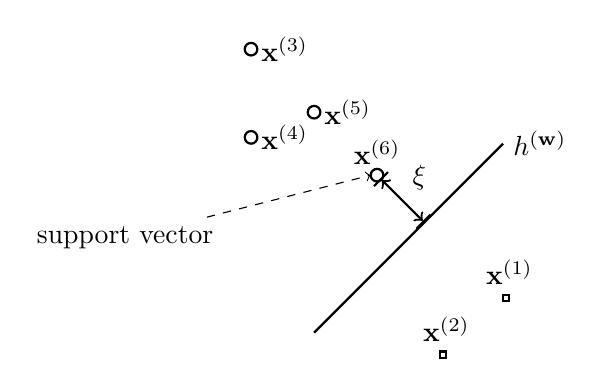
\begin{tikzpicture}[auto,scale=0.8]
					\draw [thick] (1,2) circle (0.1cm)node[anchor=west] {\hspace*{0mm}${\bf x}^{(5)}$};
					\draw [thick] (0,1.6) circle (0.1cm)node[anchor=west] {\hspace*{0mm}${\bf x}^{(4)}$};
					\draw [thick] (0,3) circle (0.1cm)node[anchor=west] {\hspace*{0mm}${\bf x}^{(3)}$};
					\draw [thick] (2,1) circle (0.1cm)node[anchor=east,above] {\hspace*{0mm}${\bf x}^{(6)}$};
					\node[] (B) at (-2,0) {support vector};
					\draw[->,dashed] (B) to (1.9,1) ; 
					\draw [|<->|,thick] (2.05,0.95)  -- (2.75,0.25)node[pos=0.5] {$\xi$} ; 
					\draw [thick] (1,-1.5) -- (4,1.5) node [right] {$h^{({\bf w})}$} ; 
					\draw [thick] (3,-1.9) rectangle ++(0.1cm,0.1cm) node[anchor=west,above]  {\hspace*{0mm}${\bf x}^{(2)}$};
					\draw [thick] (4,.-1) rectangle ++(0.1cm,0.1cm) node[anchor=west,above] {\hspace*{0mm}${\bf x}^{(1)}$};
				\end{tikzpicture}
				\caption{The SVM learns a hypothesis (or classifier) $h^{({\bf w})}$ with 
					minimal average soft-margin hinge loss. Minimizing this loss is equivalent 
					to maximizing the margin $\xi$ between the decision boundary of $h^{({\bf w})}$ 
					and each class of the training set.}
				\label{fig_svm_gls_dict}
			\end{center}
		\end{figure}
		The above basic variant of SVM is only useful if the data points from different categories can be  
		(approximately) linearly separated. For an ML application where the categories are not 
		derived from a kernel.
				\\
		See also: classification, hypothesis, map, linear regression, logistic regression, ERM, linear model, loss function, data point, feature space, maximum, hinge loss, vector, classifier, loss, decision boundary, training set, ML, kernel.},
	first={support vector machine (SVM)},
	text={SVM} 
}

\newglossaryentry{eigenvalue}
{name={eigenvalue}, plural={eigenvalues}, 
	description={We refer to a 
		number $\lambda \in \mathbb{R}$ as an eigenvalue of a square matrix $\mathbf{A} \in \mathbb{R}^{d \times d}$ 
		if there is a nonzero vector ${\bf x} \in \mathbb{R}^{d} \setminus \{ \mathbf{0} \}$ such that $\mathbf{A} {\bf x} = \lambda {\bf x}$.
		\\
		See also: matrix, vector. },
	first={eigenvalue},
	text={eigenvalue} 
}
	
\newglossaryentry{eigenvector}
{name={eigenvector}, plural={eigenvectors}, 
	description={An 
		eigenvector of a matrix $\mathbf{A} \in \mathbb{R}^{d \times d}$ 
		is a nonzero vector ${\bf x} \in \mathbb{R}^{d} \setminus \{ \mathbf{0} \}$ 
		such that $\mathbf{A} {\bf x} = \lambda {\bf x}$ with some eigenvalue $\lambda$.
				\\
		See also: matrix, vector, eigenvalue.},
	first={eigenvector},
	text={eigenvector} 
}

\newglossaryentry{evd}
{name={eigenvalue decomposition (EVD)}, 
	description={The EVD
		for a square matrix ${\bf A} \in \mathbb{R}^{d \times d}$ 
		is a factorization of the form 
		$${\bf A} = \mathbf{V} {\bm \Lambda} \mathbf{V}^{-1}.$$ 
		The columns of the matrix $\mathbf{V} = \big( {\bf v}^{(1)}, \,\ldots, \,{\bf v}^{(d)} \big)$ are the 
		eigenvectors of the matrix $\mathbf{V}$. The diagonal matrix 
		${\bm \Lambda} = {\rm diag} \big\{ \lambda_{1}, \,\ldots, \,\lambda_{d} \big\}$ 
		contains the eigenvalues $\lambda_{j}$ corresponding to the eigenvectors ${\bf v}^{(j)}$. 
		Note that the above decomposition exists only if the matrix ${\bf A}$ is diagonalizable.
				\\
		See also: matrix, eigenvector, eigenvalue.},
	first={eigenvalue decomposition (EVD)},
	text={EVD} 
}

\newglossaryentry{svd}
{name={singular value decomposition (SVD)}, 
  	description={The SVD  
  		for a matrix ${\bf A} \in \mathbb{R}^{m \times d}$ 
		is a factorization of the form 
		$${\bf A} = \mathbf{V} {\bm \Lambda} \mathbf{U}\,^{T}$$ 
		with orthonormal matrices $\mathbf{V} \in \mathbb{R}^{m \times m}$ 
		and $\mathbf{U} \in \mathbb{R}^{d \times d}$ \cite{GolubVanLoanBook}. 
		The matrix ${\bm \Lambda} \in \mathbb{R}^{m \times d}$ is 
		only nonzero along the main diagonal, whose entries $\Lambda_{j,j}$ 
		are nonnegative and referred to as singular values.
		\\
		See also: matrix. },
	first={singular value decomposition (SVD)},
	text={SVD} 
}


\newglossaryentry{tv}
{name={total variation}, 
	description={See GTV.},
	first={total variation},
	text={total variation} 
}


 \newglossaryentry{cvxclustering}
 {name={convex clustering}, 
 	description={Consider a dataset 
 		${\bf x}^{(1)}, \,\ldots, \,{\bf x}^{(m)} \in \mathbb{R}^{d}$. 
 		Convex clustering learns vectors ${\bf w}^{(1)}, \,\ldots, \,{\bf w}^{(m)}$ by minimizing 
 		$$\sum_{r=1}^{m} \left\Vert  {{\bf x}^{(r)} - {\bf w}^{(r)}} \right\Vert_{2}^2 + 
 		\alpha \sum_{i,i' \in \mathcal{V}} \left\Vert  {{\bf w}^{(i)} - {\bf w}^{(i')}} \right\Vert_{p}.$$ 
		Here, $\left\Vert  {{\bf u}} \right\Vert_{p} := \big( \sum_{j=1}^{d} |u_{j}|^{p} \big)^{1/p}$ 
		denotes the $p$-norm (for $p\geq1$).  
		It turns out that many of the optimal vectors $\widehat{{\bf w}}^{(1)}, \,\ldots, \,\widehat{{\bf w}}^{(m)}$ 
		coincide. A cluster then consists of those data points $r \in \{1, \,\ldots, \,m\}$ 
		with identical $\widehat{{\bf w}}^{(r)}$ \cite{JMLR:v22:18-694}, \cite{Pelckmans2005}. 
			\\
		See also: dataset, convex, clustering, vector, norm, cluster, data point. },
 	first={convex clustering},
	text={convex clustering} 
}


\newglossaryentry{gdmethods}
{name={gradient-based methods}, 
	description={Gradient-based 
		methods are iterative techniques for finding the minimum (or maximum) 
		of a differentiable objective function of the model parameters. These 
		methods construct a sequence of approximations to an optimal choice for 
		model parameters that results in a minimum (or maximum) value of the objective function. 
		As their name indicates, gradient-based methods use the gradients of the objective function 
		evaluated during previous iterations to construct new, (hopefully) improved model parameters. 
		One important example of a gradient-based method is GD.
				\\
		See also: gradient, minimum, maximum, differentiable, objective function, model parameters, GD.},
	first={gradient-based methods},
	text={gradient-based methods} 
}


\newglossaryentry{sgd}
{name={subgradient descent}, 
	description={Subgradient 
		descent is a generalization of GD that does not require differentiability of the 
		function to be minimized. This generalization is obtained by replacing the concept 
		of a gradient with that of a subgradient. Similar to gradients, subgradients 
		allow us to construct local approximations of an objective function. The objective function 
		might be the empirical risk $\widehat{L}\big( h^{({\bf w})} \big| \mathcal{D} \big)$ viewed 
		as a function of the model parameters ${\bf w}$ that select a hypothesis $h^{({\bf w})} \in \mathcal{H}$.
				\\
		See also: subgradient, generalization, GD, function, gradient, objective function, empirical risk, model parameters, hypothesis.},
	first={subgradient descent},
	text={subgradient descent} 
}
	
\newglossaryentry{stochGD}
{name={stochastic gradient descent (SGD)}, 
	description={SGD 
		is obtained from GD by replacing the gradient of the objective function 
		with a stochastic approximation. A main application of SGD
		is to train a parameterized model via ERM on a training set $\mathcal{D}$ that 
		is either very large or not readily available (e.g., when data points are stored 
		in a database distributed all over the planet). To evaluate the gradient of the 
		empirical risk (as a function of the model parameters ${\bf w}$), 
		we need to compute a sum $\sum_{r=1}^{m} \nabla_{{\bf w}} L\left({\bf z}^{(r)},{\bf w} \right)$  
		over all data points in the training set. We obtain a stochastic 
		approximation to the gradient by replacing the sum $\sum_{r=1}^{m} \nabla_{{\bf w}} L\left({\bf z}^{(r)},{\bf w} \right)$ 
		with a sum $\sum_{r \in \mathcal{B}} \nabla_{{\bf w}} L\left({\bf z}^{(r)},{\bf w} \right)$ 
		over a randomly chosen subset $\mathcal{B} \subseteq \{1, \,\ldots, \,m\}$ (see Fig. \ref{fig_sgd_approx_dict}). 
		We often refer to these randomly chosen data points as a batch. 
		The batch size $|\mathcal{B}|$ is an important parameter of SGD. 
		SGD with $|\mathcal{B}|> 1$ is referred to as mini-batch SGD \cite{Bottou99}. 		
		\begin{figure}[H]
			\centering
			\begin{tikzpicture}[scale=1.5, >=stealth]
				\draw[thick, blue, domain=0.5:2.5, samples=100] plot (\x, {(\x-1.5)^2 + 1});
				\node[blue,above] at (0.5, 2) {$\sum\limits_{r=1}^{m}$};
				\draw[thick, red, domain=1:3, samples=100] plot (\x, {(\x-2)^2 + 0.5});
				\node[red] at (3.3, 1.5) {$\sum\limits_{r \in \mathcal{B}}$};
			\end{tikzpicture}
		\caption{SGD for ERM approximates the gradient 
		$\sum_{r=1}^{m} \nabla_{{\bf w}} L\left({\bf z}^{(r)},{\bf w} \right)$ 
		by replacing the 
		sum over all data points in the training set (indexed by $r=1, \,\ldots, \,m$) 
		with a sum over a randomly chosen subset $\mathcal{B} \subseteq \{1, \,\ldots, \,m\}$.\label{fig_sgd_approx_dict}}
		\end{figure}
		See also: GD, gradient, objective function, stochastic, model, ERM, training set, data point, empirical risk, function, model parameters, batch, parameter.},
	first={stochastic gradient descent (SGD)},
	text={SGD} 
}


\newglossaryentry{onlineGD}
{name={online gradient descent (online GD)}, 
	description={Consider  an ML method that learns model parameters 
		${\bf w}$ from some parameter space $\mathcal{W} \subseteq \mathbb{R}^{d}$. 
		The learning process uses data points ${\bf z}^{(t)}$ that arrive at consecutive time instants $t=1, \,2, \,\dots$. 
		Let us interpret the data points ${\bf z}^{(t)}$ as iid copies 
		of an RV ${\bf z}$. The risk $\mathbb{E} \{ L\left({\bf z},{\bf w} \right) \}$ of a 
		hypothesis $h^{({\bf w})}$ can then (under mild conditions) be obtained as the limit 
		$\lim_{T\rightarrow \infty} (1/T)\sum_{t=1}\,^{T} L\left({\bf z}^{(t)},{\bf w} \right)$. 
		We might use this limit as the objective function for learning the model parameters ${\bf w}$. 
		Unfortunately, this limit can only be evaluated if we wait infinitely long in order to collect all data points. 
		Some ML applications require methods that learn online, i.e., as soon as a new data point ${\bf z}^{(t)}$ 
		arrives at time $t$, we update the current model parameters ${\bf w}^{(t)}$. Note that 
		the new data point ${\bf z}^{(t)}$ contributes the component $L\left({\bf z}^{(t)},{\bf w} \right)$ 
		to the risk. As its name suggests, online GD updates ${\bf w}^{(t)}$ via a (projected) gradient step such that
		\begin{equation} 
			\label{equ_def_ogd_dict}
 			{\bf w}^{(t+1)} := P_{\mathcal{W}}\big( {\bf w}^{(t)} - \eta_{t} \nabla_{{\bf w}} L\left({\bf z}^{(t)},{\bf w} \right)\big) . 
		\end{equation} 
		Note that \eqref{equ_def_ogd_dict} is a gradient step for the current component $L\left({\bf z}^{(t)},\cdot \right)$ 
		of the risk. The update \eqref{equ_def_ogd_dict} ignores all previous components $L\left({\bf z}^{(t')},\cdot \right)$, 
		for $t' < t$. It might therefore happen that, compared to ${\bf w}^{(t)}$, the updated model parameters 
		${\bf w}^{(t+1)}$ increase the retrospective average loss $\sum_{t'=1}^{t-1} L\left({\bf z}^{(t')},\cdot \right)$. 
		However, for a suitably chosen learning rate $\eta_{t}$, online GD can be shown 
		to be optimal in practically relevant settings. By optimal, we mean that the model parameters 
		${\bf w}^{(T+1)}$ delivered by online GD after observing $T$ data points ${\bf z}^{(1)}, \,\ldots, \,{\bf z}^{(T)}$ 
		are at least as good as those delivered by any other learning method \cite{HazanOCO}, \cite{GDOptimalRakhlin2012}. 
\begin{figure}[H]
	\begin{center}
\begin{tikzpicture}[x=1.5cm,scale=1.5, every node/.style={font=\footnotesize}]
	\draw[->] (0.5, 0) -- (5.5, 0) node[below] {};
	\foreach \x in {1, 2, 3, 4, 5} {
		\draw (\x, 0.1) -- (\x, -0.1) node[below] {$t=\x$};
	}
	\foreach \x/\y in {1/2.5, 2/1.8, 3/2.3, 4/1.5, 5/2.0} {
		\fill[black] (\x, \y) circle (2pt) node[above right] {${\bf z}^{(\x)}$};
	}
	\foreach \x/\y in {1/1.0, 2/1.6, 3/1.8, 4/2.2, 5/1.9} {
		\fill[blue] (\x, \y) circle (2pt) node[below left] {${\bf w}^{(\x)}$};
	}
	\foreach \x/\y/\z in {1/2.5/1.0, 2/1.8/1.6, 3/2.3/2.0, 4/1.5/1.8, 5/2.0/1.9} {
		\draw[dashed, gray] (\x, \y) -- (\x, \z);
	}
	\end{tikzpicture}
\end{center} 
\caption{An instance of online GD that updates the model parameters ${\bf w}^{(t)}$ 
using the data point ${\bf z}^{(t)} = x^{(t)}$ arriving at time $t$. 
This instance uses the squared error loss $L\left({\bf z}^{(t)},w \right) = (x^{(t)} - w)^{2}$.}
\end{figure}
		See also: ML, model parameters, parameter space, data point, iid, RV, risk, hypothesis, objective function, GD, gradient step, loss, learning rate, squared error loss.},
	first={online gradient descent (online GD)},
	text={online GD}
}

\newglossaryentry{pca}
{name={principal component analysis (PCA)}, 
	description={PCA 
		determines a linear feature map such that the new features 
		allow us to reconstruct the original features with the minimum reconstruction error \cite{MLBasics}.
				\\
		See also: feature map, feature, minimum.},
	first={principal component analysis (PCA)},
	text={PCA} 
}
	
\newglossaryentry{loss}
{name={loss}, 
	description={ML methods use a 
		loss function $L\left({\bf z},h \right)$ to measure the error incurred 
		by applying a specific hypothesis to a specific data point. With a
		slight abuse of notation, we use the term loss for both the loss function $L$ 
		itself and the specific value $L\left({\bf z},h \right)$, for a data point ${\bf z}$ 
		and hypothesis $h$.
				\\
		See also: ML, loss function, hypothesis, data point.},
	first={loss},
	text={loss} 
}

\newglossaryentry{lossfunc}
{name={loss function}, 
	description={A loss function is a map 
		$$L: \mathcal{X} \times \mathcal{Y} \times \mathcal{H} \rightarrow \mathbb{R}_{+}: \big( \big({\bf x},y\big),
		 h\big) \mapsto  L\left(({\bf x},y),h \right).$$
		It assigns a nonnegative real number (i.e., the loss) $L\left(({\bf x},y),h \right)$
		to a pair that consists of a data point, with features ${\bf x}$ 
		and label $y$, and a hypothesis $h \in \mathcal{H}$. The 
		value $L\left(({\bf x},y),h \right)$ quantifies the discrepancy 
		between the true label $y$ and the prediction $h({\bf x})$. 
		Lower (closer to zero) values $L\left(({\bf x},y),h \right)$ indicate a smaller 
		discrepancy between prediction $h({\bf x})$ and label $y$. 
		Fig. \ref{fig_loss_function_gls_dict} depicts a loss function for a given data point, 
		with features ${\bf x}$ and label $y$, as a function of the hypothesis $h \in \mathcal{H}$. 
		\begin{figure}[H]
			\begin{center}
				\begin{tikzpicture}[scale = 0.7]
					\begin{axis}
						[axis x line=center,
						axis y line=center,
						xlabel={},
						xlabel style={below right},
						ylabel style={above right},
						xtick=\empty,
						ytick=\empty,
						xmin=-4,
						xscale = 1.4, 
						xmax=4,
						ymin=-0.5,
						ymax=2.5
						]
						\addplot [red, thick] {ln(1 + exp(-x))};    
					\end{axis}
					\node [above,centered,xshift=-5pt] at (1,5) {$L\left(({\bf x},y),h \right)$};
					\node [above] at (10,1) {hypothesis $h$};
						\node [right] at (4,6) {loss};
				\end{tikzpicture}
			\end{center}
			\vspace*{-7mm}
			\caption{Some loss function $L\left(({\bf x},y),h \right)$ for a fixed data point, with 
				feature vector ${\bf x}$ and label $y$, and a varying hypothesis $h$. 
				ML methods try to find (or learn) a hypothesis that incurs minimal loss.}
			\label{fig_loss_function_gls_dict}
		\end{figure}
		See also: loss, function, map, data point, feature, label, hypothesis, prediction, feature vector, ML.},
 	first={loss function},
 	text={loss function} 
}

\newglossaryentry{decisiontree}
{name={decision tree}, plural={decision trees}, 
	description={A 
		decision tree is a flowchart-like representation of a hypothesis map $h$. 
		More formally, a decision tree is a directed graph containing a root node that reads 
		in the feature vector ${\bf x}$ of a data point. The root node then forward 
		the data point to one of its child nodes based on some elementary test on the features ${\bf x}$. 
		If the receiving child node is not a leaf node, i.e., it has child nodes itself, 
	  	it represents another test. Based on the test result, the data point is forwarded 
	   	to one of its descendants. This testing and forwarding of the data point is continued 
	  	until the data point ends up in a leaf node without any children. 
		\begin{figure}[H]
		\begin{minipage}{.45\textwidth}
		\scalebox{1}{
		\begin{tikzpicture}
			\node[fill=black, circle, inner sep=2pt, label=above:{$\| {\bf x}-\mathbf{u} \| \leq \varepsilon$?}] (A) {};	
			\node[fill=black, circle, inner sep=2pt, below left=1.5cm and 1cm of A, label=left:{$h({\bf x}) = \hat{y}_1$}] (B) {};
			\node[fill=black, circle, inner sep=2pt, below right=1.5cm and 1cm of A, label=right:{$\| {\bf x} - \mathbf{v} \| \leq \varepsilon$?}] (C) {};
			\node[fill=black, circle, inner sep=2pt, below left=1.5cm and 1cm of C, label=left:{$h({\bf x}) = \hat{y}_2$}] (D) {};
			\node[fill=black, circle, inner sep=2pt, below right=1.5cm and 1cm of C, label=right:{$h({\bf x}) =\hat{y}_3$}] (E) {};
			\draw[line width=1.5pt, ->] (A) -- (B) node[midway, left] {no};
			\draw[line width=1.5pt, ->] (A) -- (C) node[midway, right] {yes};
			\draw[line width=1.5pt, ->] (C) -- (D) node[midway, left] {no};
			\draw[line width=1.5pt, ->] (C) -- (E) node[midway, right] {yes};
			\node at (0.7,-4.5) {\selectfont (a)};
		\end{tikzpicture}
		}
		\end{minipage}	
		\hspace*{15mm}
		\begin{minipage}{.45\textwidth}
		\hspace*{15mm}
		\begin{tikzpicture}
		\draw (-2,2) rectangle (2,-2);
		\begin{scope}
			\clip (-0.5,0) circle (1cm);
			\clip (0.5,0) circle (1cm);
			\fill[color=gray] (-2,1.5) rectangle (2,-1.5);
		\end{scope}
		\draw (-0.5,0) circle (1cm);
		\draw (0.5,0) circle (1cm);
		\draw[fill] (-0.5,0) circle [radius=0.025];
		\node [below right, red] at (-0.5,0) {$\hat{y}_{3}$};
		\node [below left, blue] at (-0.7,0) {$\hat{y}_{2}$};
		\node [above left] at (-0.7,1) {$\hat{y}_{1}$};
		\node [left] at (-0.4,0) {$\mathbf{u}$};
		\draw[fill] (0.5,0) circle [radius=0.025];
		\node [right] at (0.6,0) {$\mathbf{v}$};
		\node at (0,-3.5) {\selectfont (b)};
		\end{tikzpicture}
		\end{minipage}
		\caption{(a) A decision tree is a flowchart-like representation of a piecewise constant hypothesis $h: \mathcal{X} \rightarrow \mathbb{R}$.  
		Each piece is a decision region $\mathcal{R}_{\hat{y}} := \big\{ {\bf x} \in  \mathcal{X}: h({\bf x}) = \hat{y} \big\}$. 
		The depicted decision tree can be applied to numeric feature vectors, i.e., $\mathcal{X} \subseteq \mathbb{R}^{d}$. It is parameterized 
		by the threshold $\varepsilon>0$ and the vectors ${\bf u}, {\bf v} \in \mathbb{R}^{d}$. 
		(b) A decision tree partitions the feature space $\mathcal{X}$ into decision regions. Each decision region  
		$\mathcal{R}_{\hat{y}} \!\subseteq\!\mathcal{X}$ corresponds to a specific leaf node in the decision tree.}
		\label{fig_decision_tree_dict}
		\end{figure} 
		See also: decision region.},
	  first={decision tree},
	  text={decision tree} 
}


\newglossaryentry{API} 
{name={application programming interface (API)},
		description={An  API is a formal mechanism that 
			allows software components to interact in a structured and modular way \cite{RestfulBook2013}.
			In the context of ML, APIs are commonly used to provide access to a trained ML model. 
			Users—whether humans or machines—can submit the feature vector of a data point and receive 
			a corresponding prediction. Suppose a trained ML model is defined 
			as $\widehat{h}(x) := 2 x + 1$. Through an API, a user 
			can input $x = 3$ and receive the output $\widehat{h}(3) = 7$ 
			without knowledge of the detailed structure of the ML model or its training. 
			In practice, the model is typically deployed on a server connected to the Internet. 
			Clients send requests containing feature values to the server, which responds with 
			the computed prediction $\widehat{h}({\bf x})$. APIs promote modularity 
			in ML system design, i.e., one team can develop and train the model, while another team
			handles integration and user interaction. Publishing a trained model via an API also 
			offers practical advantages. For instance, the server can centralize computational resources that 
			are required to compute predictions. Furthermore, the internal structure of the model remains 
			hidden—which is useful for protecting intellectual property or trade secrets. 
			However, APIs are not without risk. Techniques such as model inversion can potentially reconstruct a 
			model from its predictions using carefully selected feature vectors.
					\\
			See also: ML, model, feature vector, data point, prediction, feature, model inversion.},
		first={application programming interface (API)},
		text={API}
}

\newglossaryentry{modelinversion}
{name={model inversion},
  description={A model inversion is a form of privacy attack on an ML system. 
  	An adversary seeks to infer sensitive attributes of individual data points by exploiting partial access 
  	to a trained model $\hat{h} \in \mathcal{H}$. This access typically consists of 
  	querying the model for predictions $\hat{h}({\bf x})$ using carefully chosen inputs. 
  	Basic model inversion techniques have been demonstrated in the context of facial image 
  	classification, where images are reconstructed using the (gradient of) model outputs 
  	combined with auxiliary information such as a person’s name \cite{Fredrikson2015} (see Fig. \ref{fig_model_inv_dict}).
  	\begin{figure}[H]
		\begin{center}
		\begin{tikzpicture}[scale=1.5]
  		
  		\draw[->] (-0.5,0) -- (5.5,0) node[right] {face image ${\bf x}$};
  		\draw[->] (0,-0.2) -- (0,2.5) node[above] {name};
  		
  		\draw[thick, domain=0.5:5, samples=100, smooth, variable=\x, name path=sigmoid] 
  		plot ({\x}, {2/(1 + exp(-3*(\x - 3)))});
  		
  		
  		\def\xval{3}
  		\pgfmathsetmacro{\yval}{2/(1 + exp(-3*(\xval - 3)))}
  		
  		\draw[dashed] (\xval,0) -- (\xval,\yval);
  		\draw[dashed] (0,\yval) -- (\xval,\yval);
  		
  		\filldraw[fill=blue!20, draw=blue] (\xval,\yval) circle (0.1);
  		\node[anchor=south east] at (-0.1,\yval) {\footnotesize ``Alexander Jung''};
  		
  		\node[anchor=north] at (\xval,-0.25) {\includegraphics[width=1cm]{assets/AlexanderJung.jpg}}; 
  		
  		\node[above right] at (4,2.2) {trained model $\hat{h}$};
  		\end{tikzpicture}
		\end{center} 
		\caption{Model inversion techniques implemented in the context of facial image classification. \label{fig_model_inv_dict}}
	\end{figure}
  	See also: model, privacy attack, ML, sensitive attribute, data point, prediction, classification, gradient, trustworthy AI, privacy protection. },
  first={model inversion},
  text={model inversion}
}


\newglossaryentry{hilbertspace}
{name={Hilbert space},
	description={A Hilbert space is a complete inner 
		product space \cite{introhilbertbook}. That is, it is a vector space equipped 
		with an inner product between pairs of vectors, and it satisfies the additional requirement 
		of completeness, i.e., every Cauchy sequence of vectors converges to a limit within the space. 
		A canonical example of a Hilbert space is the Euclidean space $\mathbb{R}^{d}$, 
		for some dimension $d$, consisting of vectors ${\bf u} = \big(u_1, \,\ldots, \,u_{d}\big)\,^{T}$ 
		and the standard inner product ${\bf u}\,^{T} {\bf v}$.
				\\
		See also: vector space, vector, Euclidean space.},
	first={Hilbert space},
	text={Hilbert space}
}



\newglossaryentry{sample}
{name={sample}, plural={samples}, 
	description={A 
		finite sequence (or list) of data points ${\bf z}^{(1)}, \,\ldots, \,{\bf z}^{(m)}$ that 
		is obtained or interpreted as the realization of $m$ iid RVs 
		with a common probability distribution $p({\bf z})$. The length $m$ of 
		the sequence is referred to as the sample size.
				\\
		See also: data point, realization, iid, RV, probability distribution, sample size.},
		first={sample},
		text={sample}
}
	
\newglossaryentry{samplesize}
{name={sample size},
	description={The number of individual data points 
		contained in a dataset.
				\\
		See also: data point, dataset.},
	first={sample size},
	text={sample size}
}

\newglossaryentry{ann}
{name={artificial neural network (ANN)}, plural={ANNs},
	description={An ANN 
		is a graphical (signal-flow) representation of a function that maps 
		features of a data point at its input to a prediction 
		for the corresponding label at its output. The fundamental unit of an 
		ANN is the artificial neuron, which applies an activation function to its 
		weighted inputs. The outputs of these neurons serve as inputs for other neurons, 
		forming interconnected layers.
				\\
		See also: function, feature, data point, prediction, label, activation function.},
	first={artificial neural network (ANN)},
	text={ANN}
}


\newglossaryentry{randomforest}
{name={random forest},
	description={A random forest is a set of different decision trees. 
		Each of these decision trees is obtained by fitting a perturbed copy of 
		the original dataset.
				\\
		See also: decision tree, dataset.},
	first={random forest}, 
	text={random forest}
}

\newglossaryentry{bagging}
{name={bagging (or bootstrap aggregation)},
	description={Bagging (or bootstrap aggregation) 
		is a generic technique to improve (the robustness of) a given ML method. 
		The idea is to use the bootstrap to generate perturbed copies of a given dataset   
		and to learn a separate hypothesis for each copy. We then predict the 
		label of a data point by combining or aggregating the individual predictions 
		of each separate hypothesis. For hypothesis maps delivering numeric label 
		values, this aggregation could be implemented by computing the average of individual 
		predictions.
				\\
		See also: robustness, bootstrap.},
	first={bagging (or bootstrap aggregation)},
	text={bagging}
}


\newglossaryentry{gd}
{name={gradient descent (GD)},
	description={GD is an iterative method for 
	 	finding the minimum of a differentiable function $f: \mathbb{R}^{d} \rightarrow \mathbb{R}$. 
	 	GD generates a sequence of estimates ${\bf w}^{(0)}, \,{\bf w}^{(1)}, \,{\bf w}^{(2)}, \,\ldots$ 
	 	that (ideally) converge to a minimum of $f$. At each iteration $k$, GD refines 
	 	the current estimate ${\bf w}^{(k)}$ by taking a step in the direction of the
	 	steepest descent of a local linear approximation. This direction is given by the negative 
	 	gradient $\nabla f({\bf w}^{(k)})$ of the function $f$ at the current estimate ${\bf w}^{(k)}$. 
	 	The resulting update rule is given by
		\begin{equation} 
			\label{equ_def_GD_step_dict}
			{\bf w}^{(k\!+\!1)} = {\bf w}^{(k)} - \eta \nabla f({\bf w}^{(k)})
		\end{equation} 
		where $\eta > 0$ is a suitably small step size. For a suitably choosen step size $\eta$, 
		the update typically reduces the function value, i.e., $f({\bf w}^{(k+1)}) < f({\bf w}^{(k)})$. 
		Fig.\ \ref{fig_basic_GD_step_dict} illustrates a single GD step.
		\begin{figure}[H]
			\begin{center}
				\begin{tikzpicture}[scale=0.9]
					\draw[loosely dotted] (-4,0) grid (4,4);
					\draw[blue, ultra thick, domain=-4.1:4.1] plot (\x,  {(1/4)*\x*\x});
					\draw[red, thick, domain=2:4.7] plot (\x,  {2*\x - 4});
					\draw[<-] (4,4) -- node[right] {$\big( \Delta {\bf w}\big)\,^{T} \nabla f({\bf w}^{(k)})$} (4,2);
					\draw[->] (4,4) -- node[above] {$-\eta \nabla f({\bf w}^{(k)})$} (1,4);
					\draw[<-] (4,2) -- node[below] {$\Delta {\bf w}$} (3,2) ;
					\draw[->] (-4.25,0) -- (4.25,0) node[right] {${\bf w}$};
					\draw[->] (0,-2pt) -- (0,4.25) node[above] {$f({\bf w})$};
					\draw[shift={(0,0)}] (0pt,2pt) -- (0pt,-2pt) node[below] {$\overline{{\bf w}}$};
					\draw[shift={(4,0)}] (0pt,2pt) -- (0pt,-2pt) node[below] {${\bf w}^{(k)}$};
					\draw[shift={(1,0)}] (0pt,2pt) -- (0pt,-2pt) node[below] {${\bf w}^{(k\!+\!1)}$};
					\foreach \y/\ytext in {1/1, 2/2, 3/3, 4/4}
					\draw[shift={(0,\y)}] (2pt,0pt) -- (-2pt,0pt) node[left] {$\ytext$};  
				\end{tikzpicture}
			\end{center}
			\caption{A single gradient step \eqref{equ_def_GD_step_dict} toward the minimizer $\overline{{\bf w}}$ of $f({\bf w})$.}
			\label{fig_basic_GD_step_dict}
		\end{figure}
		See also: minimum, differentiable, gradient, step size, gradient step. },
	first={gradient descent (GD)},
	text={GD}
}

\newglossaryentry{abserr}
{name={absolute error loss},
	description={Consider a data point with features ${\bf x} \in \mathcal{X}$ and numeric 
		label $y \in \mathbb{R}$. The absolute error loss 
		incurred by a hypothesis $h: \mathcal{X} \rightarrow \mathbb{R}$ 
		is defined as $|y - h({\bf x})|$, i.e., the absolute difference between 
		the prediction $h({\bf x})$ and the true label $y$.
					\\
		See also: data point, feature, label, loss, hypothesis, prediction.},
	first={absolute error loss},
	text={absolute error loss}
}

\newglossaryentry{device}
{name={device}, plural={devices}, 
	description={Any physical system that can be used to store and process data. In the context of ML, 
		we typically mean a computer that is able to read in data points from different 
		sources and, in turn, train an ML model using these data points.
						\\
		See also: data, ML, data point, model.},
	first={device},
	text={device}
}

\newglossaryentry{llm}
{name={large language model (LLM)},
	description={LLM is an umbrella term for ML methods 
		that process and generate humanlike text. These methods typically 
		use deep nets with billions (or even trillions) of parameters. 
		A widely used choice for the network architecture is referred to as 
		Transformers \cite{vaswani2017attention}. The training of LLMs is often  
		based on the task of predicting a few words that are intentionally removed 
		from a large text corpus. Thus, we can construct labeled data points 
		simply by selecting some words from a given text as labels and the remaining 
		words as features of data points. This construction requires 
		very little human supervision and allows for generating sufficiently 
		large training sets for LLMs.
			\\
		See also: deep net, labeled data point. },
	first={large language model (LLM)},
	text={LLM}
}


\newglossaryentry{huberreg}
{name={Huber regression},
	description={Huber regression refers to ERM-based methods 
		that use the Huber loss as a measure of the prediction error. 
		Two important special cases of Huber regression are least absolute deviation regression and 
		linear regression. Tuning the threshold parameter of the Huber loss allows the user
		to trade the robustness of the absolute error loss 
		against the computational benefits of the smooth squared error loss.
					\\
		See also: least absolute deviation regression, linear regression, absolute error loss, squared error loss.},
	first={Huber regression},
	text={Huber regression}
}


\newglossaryentry{ladregression}
{name={least absolute deviation regression},
	description={Least absolute deviation regression is 
		an instance of ERM using the absolute error loss. It is a special case of Huber regression.
				\\
		See also: ERM, absolute error loss, Huber regression.},
	first={least absolute deviation regression},
	text={least absolute deviation regression}
}

\newglossaryentry{metric}
{name={metric}, plural={metrics},
	description={In its most general form, a metric is a quantitative measure used to compare or evaluate objects. 
		In mathematics, a metric measures the distance between two points and must follow specific rules, i.e., 
		the distance is always nonnegative, zero only if the points are the same, symmetric, and it satisfies the 
		triangle inequality \cite{RudinBookPrinciplesMatheAnalysis}. In ML, a metric is a quantitative measure 
		of how well a model performs. Examples include accuracy, precision, and the average $0/1$ loss 
		on a test set \cite{Goodfellow-et-al-2016}, \cite{BishopBook}. A loss function is used to train models, 
		while a metric is used to compare trained models.
		\\ 
		See also: ML, model, accuracy, $0/1$ loss, test set, loss function, loss, model selection.},
	first={metric}, 
	text={metric}
}

\newglossaryentry{bayesrisk}
{name={Bayes risk},
	description={Consider a probabilistic model with a joint probability distribution $p({\bf x},y)$ for 
		the features ${\bf x}$ and label $y$ of a data point. The 
		Bayes risk is the minimum possible risk that can be achieved by any hypothesis 
		$h: \mathcal{X} \rightarrow \mathcal{Y}$. Any hypothesis that achieves 
		the Bayes risk is referred to as a Bayes estimator \cite{LC}.
		\\
		See also: probabilistic model, risk, Bayes estimator.},
	first={Bayes risk},
	text={Bayes risk}
}
	
\newglossaryentry{bayesestimator}
{name={Bayes estimator},
	description={Consider a probabilistic model with a joint probability distribution 
		$p({\bf x},y)$ over the features ${\bf x}$ and the label $y$ 
		of a data point. For a given loss function $L\left(\cdot,\cdot \right)$, we refer to a hypothesis 
		$h$ as a Bayes estimator if its risk 
		$\mathbb{E} \left\{L\left(\left( {\bf x},y \right),h \right)\right\}$
		is the minimum achievable risk \cite{LC}. 
		Note that whether a hypothesis qualifies as a Bayes estimator depends on 
		the underlying probability distribution and the choice for the loss function $L\left(\cdot,\cdot \right)$.
		\\
		See also: probabilistic model, hypothesis, risk.},
	first={Bayes estimator},
	text={Bayes estimator}
}


\newglossaryentry{weights}
{name={weights},
	description={Consider a parameterized hypothesis space $\mathcal{H}$. We use the term 
		weights for numeric model parameters that are used to scale features or their transformations 
		in order to compute $h^{({\bf w})} \in \mathcal{H}$. A linear model uses weights 
		${\bf w}=\big(w_{1}, \,\ldots, \,w_{d}\big)\,^{T}$ to compute the linear combination 
		$h^{({\bf w})}({\bf x})= {\bf w}\,^{T} {\bf x}$. Weights are also used in ANNs 
		to form linear combinations of features or the outputs of neurons in hidden layers.
		\begin{figure}[H]
			\begin{center}
			\begin{tikzpicture}[neuron/.style={circle, draw, minimum size=1cm}, 
                    	thick, >=stealth]
			
			\node[neuron] (h1) at (0, 2) {$h_1$};
			\node[neuron] (h2) at (0, 0) {$h_2$};
			\node[neuron] (h3) at (0, -2) {$h_3$};
			
			\coordinate[right=3cm of h2] (outpoint);
			
			\node[anchor=west] at ([xshift=0.2cm]outpoint) 
    			{$z = w_1 h_1 + w_2 h_2 + w_3 h_3$};
			
			\draw[->] (h1) -- node[above] {$w_1$} (outpoint);
			\draw[->] (h2) -- node[above] {$w_2$} (outpoint);
			\draw[->] (h3) -- node[below] {$w_3$} (outpoint);
			\end{tikzpicture}
			\end{center}
			\caption{A section of an ANN that contains a hidden layer with outputs (or activations) 
			$h_{1}$,$h_{2}$, and $h_{3}$. These outputs are combined linearly to compute $z$ that can 
			be used either as output of the ANN or as input to another layer.\label{fig_weights_dict}}
		\end{figure}
		See also: hypothesis space, model parameters, feature, linear model, ANN.},
	first={weights},
	text={weights}
}
	
\newglossaryentry{probdist}
{name={probability distribution}, plural={probability distributions},
	description={To analyze ML methods, it can be useful 
		to interpret data points as iid realizations of an RV. The typical 
		properties of such data points are then governed by the probability distribution 
		of this RV. The probability distribution of a binary RV $y \in \{0,1\}$ 
		is fully specified by the probabilities $\mathbb{P}({y = 0})$ and 
		$\mathbb{P}({y=1})\!=\!1\!-\!\mathbb{P}({y=0})$. The probability 
		distribution of a real-valued RV $x \in \mathbb{R}$ might be specified 
		by a pdf $p(x)$ such that $\mathbb{P}({ x \in [a,b] }) \approx  p(a) |b-a|$. 
	    	In the most general case, a probability distribution is defined by a probability measure 
		\cite{BillingsleyProbMeasure}, \cite{GrayProbBook}.
	    		\\
		See also: iid, realization, RV, probability, pdf.},
	first={probability distribution}
	,text={probability distribution}
}
    
    
\newglossaryentry{pdf}
{name={probability density function (pdf)},
	description={The pdf $p(x)$ of a real-valued RV 
		$x \in \mathbb{R}$ is a particular representation of its probability distribution. If the pdf exists, it can 
		be used to compute the probability that $x$ takes on a value from a measurable set 
		$\mathcal{B} \subseteq \mathbb{R}$ via $\mathbb{P}({x \in \mathcal{B}}) = \int_{\mathcal{B}} p(x') d x'$ \cite[Ch. 3]{BertsekasProb}. 
		If the pdf of a vector-valued RV ${\bf x} \in \mathbb{R}^{d}$ exists, it 
        		allows us to compute the probability of ${\bf x}$ belonging to a measurable region $\mathcal{R}$ via 
        		$\mathbb{P}({{\bf x} \in \mathcal{R}}) = \int_{\mathcal{R}} p({\bf x}') d x_{1}' \,\ldots \,d x_{d}' $ \cite[Ch. 3]{BertsekasProb}.
        		\\
		See also: RV, probability distribution, probability, measurable, vector.},
	first={probability density function (pdf)},
	text={pdf}
}


\newglossaryentry{parameter}
{name={parameter},
	description={The parameter of an ML model is a tunable (i.e., learnable or adjustable) quantity that 
		allows us to choose between different hypothesis maps. For example, the linear model 
		$\mathcal{H} := \{h^{({\bf w})}: h^{({\bf w})}(x)= w_{1} x + w_{2}\}$ 
		consists of all hypothesis maps $h^{({\bf w})}(x)= w_{1} x + w_{2}$ 
		with a particular choice for the parameters ${\bf w} = \big(w_{1},w_{2}\big)\,^{T} \in \mathbb{R}^{2}$. 
		Another example of a model parameter is the weights assigned to a connection between two neurons of an ANN.
				\\
		See also: ML, model, hypothesis, map, linear model, weights, ANN.},
	first={parameter},
	text={parameter},
	firstplural={parameters}, 
 	plural={parameters}
}

\newglossaryentry{lln}
{name={law of large numbers},
	description={The law of large numbers refers to the 
		convergence of the average of an increasing (large) number of iid RVs 
		to the mean of their common probability distribution. Different instances of the 
		law of large numbers are obtained by using different notions of convergence \cite{papoulis}.
				\\
		See also: iid, RV, mean, probability distribution.},
	first={law of large numbers},
	text={law of large numbers}
}
    
\newglossaryentry{stopcrit}
{name={stopping criterion},
	description={Many ML methods use iterative algorithms 
		that construct a sequence of model parameters in order to minimize the training error. 
		For example, gradient-based methods iteratively update the parameters of a parametric model, 
		such as a linear model or a deep net. Given a finite amount of computational 
		resources, we need to stop updating the parameters after a finite number of iterations. 
		A stopping criterion is any well-defined condition for deciding when to stop updating.
				\\
		See also: algorithm, gradient-based methods.},
	first={stopping criterion},
	firstplural={stopping criteria},
	plural={stopping criteria}, 
	text={stopping criterion}
}

\newglossaryentry{kCV}
{name={$k$-fold cross-validation ($k$-fold CV)},
sort={k-fold CV},
	description={$k$-fold CV is a 
		method for learning and validating a hypothesis using a given dataset. 
		This method divides the dataset evenly into $k$ subsets or folds 
		and then executes $k$ repetitions of model training (e.g., via ERM) and validation. 
		Each repetition uses a different fold as the validation set and the remaining $k-1$ folds 
		as a training set. The final output is the average of the validation errors obtained 
		from the $k$ repetitions.
				\\
		See also: ERM, validation, validation set, training set, validation error.},
	first={$k$-fold cross-validation ($k$-fold CV)},
	text={$k$-fold CV}
}

\newglossaryentry{jacobimethod}
{name={Jacobi method},
	description={The Jacobi method is an algorithm  
		for solving systems of linear equations (i.e., a linear system) of the form ${\bf A}{\bf x}= \mathbf{b}$.  
		Here, ${\bf A} \in \mathbb{R}^{d \times d}$ is a square matrix with 
		nonzero main diagonal entries. The method constructs a sequence ${\bf x}^{(0)}, \,{\bf x}^{(1)}, \,\ldots$ 
		by updating each entry of $\mathbf{x}^{(k)}$ according to 
		\[
		x_i^{(k+1)} = \frac{1}{a_{ii}} \left( b_i - \sum_{j \neq i} a_{ij} x_j^{(k)} \right).
		\]
		Note that all entries $x^{(k)}_{1}, \,\ldots, \,x^{(k)}_{d}$ are updated simultaneously.
		The above iteration converges to a solution, i.e., $\lim_{k \rightarrow \infty} {\bf x}^{(k)}={\bf x}$, 
		under certain conditions on the matrix ${\bf A}$, e.g., being strictly 
		diagonally dominant or symmetric positive  definite \cite{GolubVanLoanBook}, \cite{StrangLinAlg2016}, \cite{Horn91}. 
		Jacobi-type methods are appealing for large linear systems due to their parallelizable structure \cite{ParallelDistrBook}.
		We can interpret the Jacobi method as a fixed-point iteration. Indeed, using the decomposition ${\bf A} = {\bf D} + {\bf R}$, with ${\bf D}$ being the 
		diagonal of ${\bf A}$, allows us to rewrite the linear equation ${\bf A} {\bf x} = {\bf b}$ as a fixed-point equation  
		\[
		\mathbf{x} = \underbrace{{\bf D}^{-1}(\mathbf{b} - {\bf R} \mathbf{x})}_{\mathcal{F} {\bf x}}
		\]
		which leads to the iteration ${\bf x}^{(k+1)} = {\bf D}^{-1}(\mathbf{b} - {\bf R} {\bf x}^{(k)})$.
		\\
		As an example, for the linear equation ${\bf A} \mathbf{x} = \mathbf{b}, \text{where}$
		 \[
		 {\bf A} = \begin{bmatrix}
		 	a_{11} & a_{12} & a_{13} \\
		 	a_{21} & a_{22} & a_{23} \\
		 	a_{31} & a_{32} & a_{33}
		 \end{bmatrix}, \quad
		 \mathbf{b} = \begin{bmatrix}
		 	b_1 \\
		 	b_2 \\
		 	b_3
		 \end{bmatrix}
		 \]
		 the Jacobi method updates each component of \( \mathbf{x} \) as follows:
		 \[
		 \begin{aligned}
		 	x_1^{(k+1)} &= \frac{1}{a_{11}} \left( b_1 - a_{12} x_2^{(k)} - a_{13} x_3^{(k)} \right); \\
		 	x_2^{(k+1)} &= \frac{1}{a_{22}} \left( b_2 - a_{21} x_1^{(k)} - a_{23} x_3^{(k)} \right); \\
		 	x_3^{(k+1)} &= \frac{1}{a_{33}} \left( b_3 - a_{31} x_1^{(k)} - a_{32} x_2^{(k)} \right).
		 \end{aligned}
		 \]
		See also: algorithm, matrix, fixed-point iteration, optimization method.},
	text={Jacobi method}, 
	first={Jacobi method}
}
	
\newglossaryentry{renyidiv}
{name={R\'enyi divergence}, 
sort={Renyi},
	description={The R\'enyi divergence measures the (dis)similarity 
		between two probability distributions \cite{RenyiInfo95}.
				\\
		See also: probability distribution.}, 
	first={R\'enyi divergence}, 
	text={R\'enyi divergence}
} 

\newglossaryentry{nonsmooth}
{name={non-smooth},
	description={We refer to a function as non-smooth if it is not 
		smooth \cite{nesterov04}.
				\\
		See also: function, smooth.},
	first={non-smooth},
	text={non-smooth}
}

\newglossaryentry{convex}
{name={convex},
	description={A subset $\mathcal{C} \subseteq \mathbb{R}^{d}$ of the 
		Euclidean space $\mathbb{R}^{d}$ is referred to as convex if it contains 
		the line segment between any two points ${\bf x}, {\bf y}\!\in\!\mathcal{C}$ in that set. A function  
		$f\!:\!\mathbb{R}^{d}\!\rightarrow\!\mathbb{R}$ 
		is convex if its epigraph $\big\{ \big( {\bf w}\,^{T},t \big)\,^{T}\!\in\!\mathbb{R}^{d\!+\!1}\!:\!t\!\geq\!f({\bf w}) \}$ 
		is a convex set \cite{BoydConvexBook}. We illustrate one example of a convex set 
		and a convex function in Fig. \ref{fig_convex_set_function_dict}. 
		\begin{figure}[H]
		\begin{center}
			\begin{tikzpicture}
				\fill[blue!20, opacity=0.5] (-3,0) ellipse (2 and 1.2); 
				\draw[thick] (-3,0) ellipse (2 and 1.2);
				\filldraw[black] (-3.7,0.2) circle (2pt) node[left] {${\bf w}$};
				\filldraw[black] (-2.3,-0.5) circle (2pt) node[right] {${\bf w}'$};
				\draw[thick] (-3.7,0.2) -- (-2.3,-0.5);
				\node at (-1.2,-1.0) {$\mathcal{C}$};
				\node at (-3,-2.4) {(a)};
				\begin{scope}[shift={(5,-1)}]
					\draw[thick, domain=-2:2, smooth, variable=\x] 
					plot ({\x}, {0.5*\x*\x});
					\fill[blue!30, opacity=0.5] 
					plot[domain=-1.5:1.5, smooth] ({\x}, {0.5*\x*\x}) -- 
					(2, {0.5*2*2}) -- 
					(-2, {0.5*2*2}) -- 
					cycle;
					\node at (0,-0.4) {$f({\bf w})$};
					\node at (0,-1.4) {(b)};
				\end{scope}
			\end{tikzpicture}
			\vspace*{-8mm}
			\end{center}
			\caption{(a) A convex set $\mathcal{C} \subseteq \mathbb{R}^{d}$. 
				(b) A convex function $f: \mathbb{R}^{d} \rightarrow \mathbb{R}$.\label{fig_convex_set_function_dict}}
		\end{figure}
		See also: Euclidean space, function, epigraph.},
	first={convex},
	text={convex}
}


\newglossaryentry{smooth}
{name={smooth},
	description={A real-valued function $f: \mathbb{R}^{d} \rightarrow \mathbb{R}$ 
		is smooth if it is differentiable and its gradient $\nabla f({\bf w})$ is continuous at all ${\bf w} \in \mathbb{R}^{d}$  \cite{nesterov04}, \cite{CvxBubeck2015}. 
		A smooth function $f$ is referred to as $\beta$-smooth if the gradient 
		$\nabla f({\bf w})$ is Lipschitz continuous with Lipschitz constant $\beta$, i.e., 
		$$\| \nabla f({\bf w}) - \nabla f({\bf w}') \| \leq \beta \| {\bf w} - {\bf w}' \| \mbox{, for any } {\bf w},{\bf w}' \in \mathbb{R}^{d}.$$ 
		The constant $\beta$ quantifies the smoothness of the function $f$: the smaller the $\beta$, 
		the smoother $f$ is. Optimization problems with a smooth objective function can be solved effectively by gradient-based methods. 
	    	Indeed, gradient-based methods approximate the objective function locally around a current choice ${\bf w}$ 
	    	using its gradient. This approximation works well if the gradient does 
	    	not change too rapidly. We can make this informal claim precise by studying the effect of a single 
	    	gradient step with step size $\eta=1/\beta$ (see Fig. \ref{fig_gd_smooth_dict}). 
	    	\begin{figure}[H] 
	    	\begin{center} 
	    	\begin{tikzpicture}[scale=0.8, x=0.6cm,y=0.05cm]
	    		
	    		\def\hshift{0.5} 
	    		
	    		\draw[thick, dashed, domain=\hshift:8+\hshift, smooth, variable=\x] plot ({\x}, {\x^2}); 
	    		
	    		\coordinate (w) at (\hshift,{\hshift*\hshift}); 
	    		\coordinate (wkplus1) at (4+\hshift,{(4+\hshift)^2}); 
	    		\coordinate (wk) at (8+\hshift,{(8+\hshift)^2}); 
	    		
  				\draw[line width=1pt, transform canvas={yshift=-1pt}] (wk) -- +(-2, -{4*(8 + \hshift)} ) -- +(1, {2*(8 + \hshift)}); 
 				\draw[line width=1pt, transform canvas={yshift=-1pt}] (w) -- +(-1, {-{2*\hshift}} ) -- +(1, {+{2*\hshift}})  node[below] {$\nabla f({\bf w})$};

	    		\filldraw (wk) circle (2pt) node[above left] {${\bf w}^{(k)}$} node[below right, xshift=-15pt,yshift=-15pt] {$\nabla f({\bf w}^{(k)})$} ;
	    		\filldraw (w) circle (2pt) node[above right] {${\bf w}$} ;
	    		\filldraw (wkplus1) circle (2pt) node[below right] {${\bf w}^{(k+1)}\!=\!{\bf w}^{(k)}\!-\!(1/\beta)\nabla f({\bf w}^{(k)})$};
	    		    
	    		\draw[dashed] (wk) -- ($(8,0) + (wk)$) ; 
	    		\draw[dashed] (wkplus1) -- ($(12,0) + (wkplus1)$) ; 
	    		 \draw[<->, thick] ($(4,0) + (wk)$) -- ($(8,0) + (wkplus1)$) 
	    		node[midway, right] {$ f\big({\bf w}^{(k)}\big)\!-\!f\big({\bf w}^{(k+1)}\big)\!\geq\!\frac{1}{2\beta}\left\Vert  {\nabla f({\bf w}^{(k)})} \right\Vert_{2}^{2}$};


	    	\end{tikzpicture}
	    	\end{center}
	    	\caption{Consider an objective function $f({\bf w})$ that is $\beta$-smooth. 
	    		Taking a gradient step, with step size $\eta = 1/\beta$, decreases the 
	    		objective by at least ${1}/{2\beta}\left\Vert  {\nabla f({\bf w}^{(k)})} \right\Vert_{2}^{2}$ \cite{nesterov04}, \cite{CvxBubeck2015}, \cite{CvxAlgBertsekas}. 
	    		Note that the step size $\eta = 1/\beta$ becomes larger for smaller $\beta$. Thus, 
	    		for smoother objective functions (i.e., those with smaller $\beta$), 
				we can take larger steps. \label{fig_gd_smooth_dict}}
	    	\end{figure}
		See also: function, differentiable, gradient, optimization problem, objective function, gradient-based methods, gradient step, step size.},
	first={smooth},
	text={smooth}
}

\newglossaryentry{paramspace}
{name={parameter space},
	description={The parameter space $\mathcal{W}$ of 
		an ML model $\mathcal{H}$ is the set of all feasible choices for the 
		model parameters (see Fig. \ref{fig_param_space_dict}). Many important ML methods 
		use a model that is parameterized by vectors of the Euclidean space $\mathbb{R}^{d}$. 
		Two widely used examples of parameterized models are linear models 
		and deep nets. The parameter space is then often a subset $\mathcal{W} \subseteq \mathbb{R}^{d}$, 
		e.g., all vectors ${\bf w} \in \mathbb{R}^{d}$ with a norm smaller than one.
		\begin{figure}[H]
			\begin{center}
			\begin{tikzpicture}
				
				\node[ellipse, minimum width=3cm, minimum height=2cm, draw, thick] (paramspace) {};
				\node[below=0.1cm of paramspace] {parameter space $\mathcal{W}$};
				
				\node[black, circle, inner sep=2pt, fill] (theta1) at ($(paramspace.north west) + (1, -1)$) {};
				\node[left=0.01cm of theta1] {${\bf w}$};
				\node[black, circle, inner sep=2pt, fill] (theta2) at ($(paramspace.south east) + (-1.5, 1)$) {};
				\node[left=0.01cm of theta2] {${\bf w}'$};
				
				\node[ellipse, minimum width=7cm, minimum height=3cm, draw, thick, right=4cm of paramspace] (plotcloud) {};
				\node[above=0.2cm of plotcloud] {model $\mathcal{H}$};
				
				\node (plot1start) at ($(plotcloud.south west) + (0.2, 0.2)$) {};
				
				
				
				\draw[thick, red] (plot1start) .. controls ++(0.8, 1) and ++(-0.8, -0.8) .. ($(plotcloud.south west) + (2.8, 0.8)$) node[anchor=west] {$h^{({\bf w})}$};
				
				\node (plot2start) at ($(plotcloud.south west) + (1.0, 1.2)$) {};
			
			
				
				\draw[thick, blue] (plot2start) .. controls ++(0.8, 0.5) and ++(-0.8, -0.8) .. ($(plotcloud.south west) + (2.8, 2.1)$) node[anchor=west] {$h^{({\bf w}')}$};
				
				\draw[thick, ->, bend right=20] (theta1) to ($(plot1start) + (0,0)$);
				\draw[thick, ->, bend left=20] (theta2) to (plot2start);
			\end{tikzpicture}
			\end{center} 
			\caption{The parameter space $\mathcal{W}$ of an ML model $\mathcal{H}$ consists of all 
			feasible choices for the model parameters. Each choice ${\bf w}$ for the model parameters 
			selects a hypothesis map $h^{({\bf w})} \in \mathcal{H}$.
				 \label{fig_param_space_dict}} 
			\end{figure}
			See also: parameter, model, model parameters.},
		first={parameter space},
		text={parameter space}
}

\newglossaryentry{datanorm}
{name={data normalization},
	description={Data normalization refers to transformations 
		applied to the feature vectors of data points to improve the ML method's 
		statistical aspects or computational aspects. For example, in linear regression with gradient-based methods using 
		a fixed learning rate, convergence depends on controlling the norm of feature vectors 
		in the training set. A common approach is to normalize feature vectors such that their 
		norm does not exceed one \cite[Ch.\ 5]{MLBasics}.
				\\
		See also: data, feature vector, data point, ML, statistical aspects, computational aspects, linear regression, gradient-based methods, learning rate, norm, training set.},
	first={data normalization},
	text={data normalization}
}

\newglossaryentry{dataaug}
{name={data augmentation},
	description={Data augmentation methods add synthetic data points 
		to an existing set of data points. These synthetic data points are obtained by 
		perturbations (e.g., adding noise to physical measurements) or transformations 
		(e.g., rotations of images) of the original data points. These perturbations and 
		transformations are such that the resulting synthetic data points should 
		still have the same label. As a case in point, a rotated cat image is still 
		a cat image even if their feature vectors (obtained by stacking pixel color intensities) 
		are very different (see Fig. \ref{fig_symmetry_dataaug_dict}). Data augmentation can be an 
		efficient form of regularization.
		\begin{figure}[H]
		\begin{center}
			\begin{tikzpicture}
				
				\newcommand{\xshift}{0.5}
				\newcommand{\yshift}{2}
				
				
  				\draw[very thick, blue] plot[smooth, tension=1] coordinates {(0,0) (2,1) (4,0) (6,-1) (8,0)};
  				\node[blue, right] at (0,0) {\textbf{cat}};
  				\draw[very thick, red, dashed] plot[smooth, tension=1] coordinates {(0 + \xshift,0 + \yshift) (2 + \xshift,1 + \yshift) (4 + \xshift,0 + \yshift) (6 + \xshift,-1 + \yshift) (8 + \xshift,0 + \yshift)};
  				\node[red, right] at (8 + \xshift,0 + \yshift) {\textbf{no cat}};
				\fill[blue] (2,1) circle (2pt) node[above] {${\bf x}^{(1)}$};
				\fill[blue] (6,-1) circle (2pt) node[above] {${\bf x}^{(2)}$};
				  
				  \draw[->, thin, >=latex, line width=0.5pt] (2,1) to[out=240, in=240] node[midway, below] {$\mathcal{T}^{(\eta)}$} (6,-1);
			  \end{tikzpicture}
			  \vspace*{-11mm}
		\end{center}
		\caption{Data augmentation exploits intrinsic symmetries of data points in 
		    some feature space $\mathcal{X}$. We can represent a symmetry by 
		    an operator $\mathcal{T}^{(\eta)}: \mathcal{X} \rightarrow \mathcal{X}$,
		    parameterized by some number $\eta \in \mathbb{R}$. For example, $\mathcal{T}^{(\eta)}$ 
		    might represent the effect of rotating a cat image by $\eta$ degrees. A data point 
		    with feature vector ${\bf x}^{(2)} = \mathcal{T}^{(\eta)} \big({\bf x}^{(1)} \big)$ must 
		    have the same label $y^{(2)}=y^{(1)}$ as a data point 
		    with feature vector ${\bf x}^{(1)}$.\label{fig_symmetry_dataaug_dict}}
		 \end{figure}
		See also: data, data point, label, feature vector, regularization, feature space. },
	first={data augmentation},
	text={data augmentation}
}
	
	
\newglossaryentry{localdataset}
{name={local dataset}, plural={local datasets}, 
	description={The concept of a local dataset is 
		in between the concept of a data point and a dataset. A local dataset consists of several 
		individual data points characterized by features and labels. 
		In contrast to a single dataset used in basic ML methods, a local dataset is also 
		related to other local datasets via different notions of similarity. These similarities 
		might arise from probabilistic models or communication infrastructure and 
		are encoded in the edges of an FL network.
				\\
		See also: dataset, data point, feature, label, ML, probabilistic model, FL network.},
		first={local dataset},
		text={local dataset}
}
	
\newglossaryentry{localmodel}
{name={local model}, plural={local models}, 
	description={Consider a collection of devices that are represented 
		as nodes $\mathcal{V}$ of an FL network. A local model $\mathcal{H}^{(i)}$ 
		is a hypothesis space assigned to a node $i \in \mathcal{V}$. Different nodes might be 
		assigned different hypothesis spaces, i.e., in general $\mathcal{H}^{(i)} \neq \mathcal{H}^{(i')}$ for different 
		nodes $i, i' \in \mathcal{V}$. 
				\\
		See also: device, FL network, model, hypothesis space. },
	first={local model},
	text={local model}
}
	
\newglossaryentry{mutualinformation}
{name={mutual information (MI)},
 	description={The MI $I \left( {\bf x};y\right)$ 
 		between two RVs ${\bf x}$, $y$ defined on the same probability space 
 		is given by \cite{coverthomas} $$I \left( {\bf x};y\right) := 
		\mathbb{E}  \left\{ \log \frac{p ({\bf x},y)}{p({\bf x})p(y)} \right\}.$$ 
		It is a measure of how well we can estimate $y$ based 
		solely on ${\bf x}$. A large value of $I \left( {\bf x};y\right)$ indicates that 
		$y$ can be well predicted solely from ${\bf x}$. This prediction could be obtained by a 
		hypothesis learned by an ERM-based ML method. 
				\\
		See also: RV, probability space, prediction, hypothesis, ERM, ML. }, 
	first={MI}, 
	text={MI} 
}

\newglossaryentry{zerogradientcondition}
{name={zero-gradient condition},
	description={Consider the unconstrained 
		optimization problem $\min_{{\bf w} \in \mathbb{R}^{d}} f({\bf w})$  with 
			a smooth and convex objective function $f({\bf w})$. A necessary and 
			sufficient condition for a vector $\widehat{{\bf w}} \in \mathbb{R}^{d}$ 
			to solve this problem is that the gradient $\nabla f \big( \widehat{{\bf w}} \big)$ 
			is the zero vector such that
			$$\nabla f \big( \widehat{{\bf w}} \big) = \mathbf{0} \Leftrightarrow  f \big( \widehat{{\bf w}} \big) = \min_{{\bf w} \in \mathbb{R}^{d}} f({\bf w}).$$ 
					\\
			See also: optimization problem, smooth, convex, objective function, vector, gradient.}, 
		first={zero-gradient condition},
		text={zero-gradient condition}
}


\newglossaryentry{edgeweight}
{name={edge weight},
	description={Each edge $\{i,i'\}$ of an FL network is 
		assigned a nonnegative edge weight $A_{i,i'}\geq0$. 
		A zero edge weight $A_{i,i'}=0$ indicates the absence 
		of an edge between nodes $i, i' \in \mathcal{V}$.
				\\
		See also: FL network.}, 
	first={edge weight},
	text={edge weight}
}


\newglossaryentry{dataminprinc}
{name={data minimization principle},
	description={European data protection regulation 
		includes a data minimization principle. This principle requires a data controller to 
		limit the collection of personal information to what is directly relevant and necessary 
		to accomplish a specified purpose. The data should be retained only for as long as 
		necessary to fulfill that purpose \cite[Article 5(1)(c)]{GDPR2016}, \cite{EURegulation2018}.
				\\
		See also: data.}, 
	first={data minimization principle},
	text={data minimization principle}
}

